%\documentclass[11pt,twoside]{article}
\documentclass[11pt,twoside]{amsart}

\usepackage{amssymb}
\usepackage{amsthm}
\usepackage{amsmath}
\usepackage{hyperref}
\usepackage{ifthen}
\usepackage{mathtools}
%\allowdisplaybreaks


\setlength{\oddsidemargin}{0cm}
\setlength{\evensidemargin}{0cm}
\setlength{\textwidth}{16cm}
\setlength{\topmargin}{-1cm}
\setlength{\textheight}{22cm}

\usepackage{etoolbox}
\let\bbordermatrix\bordermatrix
\patchcmd{\bbordermatrix}{8.75}{4.75}{}{}
\patchcmd{\bbordermatrix}{\left(}{\left[}{}{}
\patchcmd{\bbordermatrix}{\right)}{\right]}{}{}

\usepackage{graphicx}
\usepackage{tikz}
\usetikzlibrary{arrows}
\usetikzlibrary{shapes,snakes}
%\renewcommand{\arraystretch}{1.1}

\setcounter{MaxMatrixCols}{20}

\usepackage{ tikz }
\usetikzlibrary{ calc }


\theoremstyle{plain}
\newtheorem{theorem}{Theorem}
\newtheorem{lemma}[theorem]{Lemma}
\newtheorem{corollary}[theorem]{Corollary}
\newtheorem{proposition}[theorem]{Proposition}
\newtheorem{fact}[theorem]{Fact}
\newtheorem{observation}[theorem]{Observation}
\newtheorem{claim}[theorem]{Claim}

\theoremstyle{definition}
\newtheorem{definition}[theorem]{Definition}
\newtheorem{example}[theorem]{Example}
\newtheorem{conjecture}[theorem]{Conjecture}
\newtheorem{open}[theorem]{Open Problem}
\newtheorem{problem}[theorem]{Problem}
\newtheorem{question}[theorem]{Question}

\theoremstyle{remark}
\newtheorem{remark}[theorem]{Remark}
\newtheorem{note}[theorem]{Note}


\newcommand{\set}[1]{\left\{#1\right\}}

\def\tn{\textnormal}
\def\ld{\lambda}
\def\mN{\mathbb{N}}
\def\mR{\mathbb{R}}
\def\mS{\mathbb{S}}
\def\mZ{\mathbb{Z}}


\def\A{\mathcal{A}}
\def\B{\mathcal{B}}
\def\C{\mathcal{C}}

\def\E{\mathcal{E}}
\def\F{\mathcal{F}}
\def\H{\mathcal{H}}
\def\cG{\mathcal{G}}
\def\I{\mathcal{I}}
\def\J{\mathcal{J}}
\def\K{\mathcal{K}}
\def\M{\mathcal{M}}
\def\N{\mathcal{N}}
\def\O{\mathcal{O}}
\def\P{\mathcal{P}}
\def\Q{\mathcal{Q}}
\def\S{\mathcal{S}}
\def\T{\mathcal{T}}
\def\V{\mathcal{V}}
\def\W{\mathcal{W}}
\def\tn{\textnormal}
\def\ep{\epsilon}
\def\es{\emptyset}
\def\bsm{\bigg\backslash}
\def\sm{\setminus}
\def\ssm{\overline}
\def\het{\hat}
\def\a{\alpha}
\def\b{\beta}
\def\l{\ell}
\def\r{\rho}
\def\ce{\coloneqq}

\newcommand{\ignore}[1]{}
\DeclareMathOperator{\SA}{SA}
\DeclareMathOperator{\LS}{LS}
\DeclareMathOperator{\BZ}{BZ}
\DeclareMathOperator{\Las}{Las}
\DeclareMathOperator{\CG}{CG}

\DeclareMathOperator{\FRAC}{FRAC}
\DeclareMathOperator{\STAB}{STAB}

\DeclareMathOperator{\diag}{diag}
\DeclareMathOperator{\conv}{conv}
\DeclareMathOperator{\cone}{cone}
\DeclareMathOperator{\Aut}{Aut}


\title[Stable Set Polytopes with High $\LS_+$-Ranks]{\bf Stable Set Polytopes with High Lift-and-Project Ranks \\ for the Lov{\'a}sz--Schrijver SDP Operator}


\author{Yu Hin (Gary) Au \and Levent Tun{\c c}el}
\thanks{Levent Tun{\c c}el: Research of this author was supported in part by an NSERC Discovery Grant.}

\date{\today}

\keywords{stable set problem, lift and project, combinatorial optimization, semidefinite programming, integer programming}

\begin{document}

%\Large
\maketitle % typeset the title of the contribution

\begin{abstract}
We study the lift-and-project rank of the stable set polytopes of graphs with respect to the Lov{\'a}sz--Schrijver SDP operator $\LS_+$, with a particular focus on a search for relatively small graphs with high $\LS_+$-rank (the least number of iterations of the $\LS_+$ operator on the fractional stable set polytope to compute the stable set polytope). In particular, we provide families of graphs whose $\LS_+$-rank is asymptotically a linear function of its number of vertices, which is the least possible up to improvements in the constant factor (previous best result in this direction, from 1999, yielded graphs whose $\LS_+$-rank only grew with the square root of the number of vertices). We also provide several new $\LS_+$-minimal graphs, most notably a $12$-vertex graph with $\LS_+$-rank $4$, and study the properties of a vertex-stretching operation that appears to be promising in generating $\LS_+$-minimal graphs.
\end{abstract}


\section{Introduction}\label{sec1}

In combinatorial optimization, a standard approach for tackling a given problem is to encode its set of feasible solutions geometrically (e.g., via an integer program). While the exact solution set is often difficult to analyze, we can focus on relaxations of this set that have certain desirable properties (e.g., combinatorially simple to describe, approximates the underlying set of solutions well, and/or is computationally efficient to optimize over). In that regard, the \emph{lift-and-project} approach provides a systematic procedure which generates progressively tighter convex relaxations of any given $0,1$ optimization problem. In the last three decades, many procedures that fall under the lift-and-project approach have been devised (see, among others,~\cite{SheraliA90, LovaszS91, BalasCC93, Lasserre01, BienstockZ04, AuT16}), and there is an extensive body of work on their general properties and performance on a wide range of discrete optimization problems (see, for instance,~\cite{AuPhD} and the references therein).

Herein, we focus on $\LS_+$, the SDP lift-and-project operator due to Lov{\'a}sz and Schrijver~\cite{LovaszS91}, and its performance on the stable set problem of graphs. A remarkable property of $\LS_+$ is that applying one iteration of the operator to the fractional stable set polytope of a graph already yields a tractable relaxation of the stable set polytope that is stronger than the Lov{\'a}sz theta body relaxation. Thus, $\LS_+$ has been shown to perform well on the stable set problem for graphs that are perfect or ``close'' to being perfect~\cite{BianchiENT13, BianchiENT17, Wagler22, BianchiENW23}. For more analyses of various lift-and-project relaxations of the stable set problem, see (among others)~\cite{LovaszS91, Laurent03, LiptakT03, BienstockO04, EscalanteMN06, GvozdenovicL07, GiandomenicoLRS09, GiandomenicoRS13, AuT16, AuLT22}.

The worst-case behaviours of $\LS_+$ have also been studied extensively. Generally, the \emph{$\LS_+$-rank} of a set is defined to be the number of iterations it takes $\LS_+$ to return its integer hull. It is known that the $\LS_+$-rank of a set $P \subseteq [0,1]^n$ is at most $n$, and a number of elementary polytopes in $\mR^n$ have been shown to have $\LS_+$-rank $\Theta(n)$ (see, among others,~\cite{Goemans98, CookD01, GoemansT01, SchoenebeckTT07, AuT18}).

On the other hand, while the stable set problem is known to be strongly $\mathcal{NP}$-hard, hardness results for $\LS_+$ (or any other lift-and-project operator utilizing semidefinite programming) on the stable set problem have been relatively scarce. Prior to this manuscript, the worst (in terms of performance by $\LS_+$) family of examples was given by the line graphs of odd cliques. Using the fact that the $\LS_+$-rank of the fractional matching polytope of the $(2k+1)$-clique is $k$~\cite{StephenT99}, the natural correspondence between the matchings in a given graph and the stable sets in the corresponding line graph, as well as the properties of the $\LS_+$ operator, it follows that the fractional stable set polytope of the line graph of the $(2k+1)$-clique (which contains $\binom{2k+1}{2} = k(2k+1)$ vertices) has $\LS_+$-rank $k$, giving a family of graphs $G$ with $\LS_+$-rank $\Theta(\sqrt{|V(G)|})$. This lower bound on the $\LS_+$-rank of the stable set polytopes has not been improved since 1999. 

In this manuscript, we present what we believe is the first known family of graphs whose $\LS_+$-rank is asymptotically a linear function of the number of vertices. For a positive integer $k$, let $[k] \ce \set{1,2, \ldots, k}$. Given an integer $k \geq 2$, let $H_k$ be the graph where $V(H_k) \ce \set{ i_p : i \in [k], p \in \set{0,1,2}}$, and the edges of $H_k$ are
\begin{itemize}
\item
$\set{i_0, i_1}$ and $\set{i_1,i_2}$ for every $i \in [k]$;
\item
$\set{i_0, j_2}$ for all $i,j \in [k]$ where $i \neq j$.
\end{itemize}

\def\y{0.70}
\def\z{0.25}
\def\sc{2}

\begin{figure}[ht!]
\begin{center}
\begin{tabular}{ccc}

\def\x{360/3}

\begin{tikzpicture}[scale=\sc, thick,main node/.style={circle, minimum size=4mm, inner sep=0.1mm,draw,font=\tiny\sffamily}]
\node[main node] at ({ \y* cos((-1)*\x) + (1-\y)*cos((-2)*\x)},{ \y* sin((-1)*\x) + (1-\y)*sin((-2)*\x)}) (1) {$1_0$};
\node[main node] at ({cos((-1)*\x)},{sin((-1)*\x)}) (2) {$1_1$};
\node[main node] at ({ \y* cos((-1)*\x) + (1-\y)*cos(0*\x)},{ \y* sin((-1)*\x) + (1-\y)*sin((0)*\x)}) (3) {$1_2$};

\node[main node] at ({ \y* cos(0*\x) + (1-\y)*cos((-1)*\x)},{ \y* sin(0*\x) + (1-\y)*sin((-1)*\x)}) (4) {$2_0$};
\node[main node] at ({cos(0*\x)},{sin((0)*\x)}) (5) {$2_1$};
\node[main node] at ({ \y* cos(0*\x) + (1-\y)*cos(1*\x)},{ \y* sin(0*\x) + (1-\y)*sin((1)*\x)}) (6) {$2_2$};

\node[main node] at ({ \y* cos(1*\x) + (1-\y)*cos(0*\x)},{ \y* sin(1*\x) + (1-\y)*sin((0)*\x)}) (7) {$3_0$};
\node[main node] at ({cos(1*\x)},{sin((1)*\x)}) (8) {$3_1$};
\node[main node] at ({ \y* cos(1*\x) + (1-\y)*cos(2*\x)},{ \y* sin(1*\x) + (1-\y)*sin((2)*\x)}) (9) {$3_2$};

 \path[every node/.style={font=\sffamily}]
(2) edge (1)
(2) edge (3)
(5) edge (4)
(5) edge (6)
(8) edge (7)
(8) edge (9)
(1) edge (6)
(1) edge (9)
(4) edge (3)
(4) edge (9)
(7) edge (3)
(7) edge (6);
\end{tikzpicture}


&

\def\x{360/4}
\begin{tikzpicture}[scale=\sc, thick,main node/.style={circle, minimum size=4mm, inner sep=0.1mm,draw,font=\tiny\sffamily}]

\node[main node] at ({ \y* cos((-1)*\x) + (1-\y)*cos((-2)*\x)},{ \y* sin((-1)*\x) + (1-\y)*sin((-2)*\x)}) (1) {$1_0$};
\node[main node] at ({cos((-1)*\x)},{sin((-1)*\x)}) (2) {$1_1$};
\node[main node] at ({ \y* cos((-1)*\x) + (1-\y)*cos(0*\x)},{ \y* sin((-1)*\x) + (1-\y)*sin((0)*\x)}) (3) {$1_2$};

\node[main node] at ({ \y* cos(0*\x) + (1-\y)*cos((-1)*\x)},{ \y* sin(0*\x) + (1-\y)*sin((-1)*\x)}) (4) {$2_0$};
\node[main node] at ({cos(0*\x)},{sin((0)*\x)}) (5) {$2_1$};
\node[main node] at ({ \y* cos(0*\x) + (1-\y)*cos(1*\x)},{ \y* sin(0*\x) + (1-\y)*sin((1)*\x)}) (6) {$2_2$};

\node[main node] at ({ \y* cos(1*\x) + (1-\y)*cos(0*\x)},{ \y* sin(1*\x) + (1-\y)*sin((0)*\x)}) (7) {$3_0$};
\node[main node] at ({cos(1*\x)},{sin((1)*\x)}) (8) {$3_1$};
\node[main node] at ({ \y* cos(1*\x) + (1-\y)*cos(2*\x)},{ \y* sin(1*\x) + (1-\y)*sin((2)*\x)}) (9) {$3_2$};

\node[main node] at ({ \y* cos(2*\x) + (1-\y)*cos(1*\x)},{ \y* sin(2*\x) + (1-\y)*sin((1)*\x)}) (10) {$4_0$};
\node[main node] at ({cos(2*\x)},{sin(2*\x)}) (11) {$4_1$};
\node[main node] at ({ \y* cos(2*\x) + (1-\y)*cos(3*\x)},{ \y* sin(2*\x) + (1-\y)*sin((3)*\x)}) (12) {$4_2$};

 \path[every node/.style={font=\sffamily}]
(2) edge (1)
(2) edge (3)
(5) edge (4)
(5) edge (6)
(8) edge (7)
(8) edge (9)
(11) edge (10)
(11) edge (12)
(1) edge (6)
(1) edge (9)
(1) edge (12)
(4) edge (3)
(4) edge (9)
(4) edge (12)
(7) edge (3)
(7) edge (6)
(7) edge (12)
(10) edge (3)
(10) edge (6)
(10) edge (9);
\end{tikzpicture}

&

\def\x{360/5}


\begin{tikzpicture}[scale=\sc, thick,main node/.style={circle, minimum size=4mm, inner sep=0.1mm,draw,font=\tiny\sffamily}]
\node[main node] at ({ \y* cos((-1)*\x) + (1-\y)*cos((-2)*\x)},{ \y* sin((-1)*\x) + (1-\y)*sin((-2)*\x)}) (1) {$1_0$};
\node[main node] at ({cos((-1)*\x)},{sin((-1)*\x)}) (2) {$1_1$};
\node[main node] at ({ \y* cos((-1)*\x) + (1-\y)*cos(0*\x)},{ \y* sin((-1)*\x) + (1-\y)*sin((0)*\x)}) (3) {$1_2$};

\node[main node] at ({ \y* cos(0*\x) + (1-\y)*cos((-1)*\x)},{ \y* sin(0*\x) + (1-\y)*sin((-1)*\x)}) (4) {$2_0$};
\node[main node] at ({cos(0*\x)},{sin((0)*\x)}) (5) {$2_1$};
\node[main node] at ({ \y* cos(0*\x) + (1-\y)*cos(1*\x)},{ \y* sin(0*\x) + (1-\y)*sin((1)*\x)}) (6) {$2_2$};

\node[main node] at ({ \y* cos(1*\x) + (1-\y)*cos(0*\x)},{ \y* sin(1*\x) + (1-\y)*sin((0)*\x)}) (7) {$3_0$};
\node[main node] at ({cos(1*\x)},{sin((1)*\x)}) (8) {$3_1$};
\node[main node] at ({ \y* cos(1*\x) + (1-\y)*cos(2*\x)},{ \y* sin(1*\x) + (1-\y)*sin((2)*\x)}) (9) {$3_2$};

\node[main node] at ({ \y* cos(2*\x) + (1-\y)*cos(1*\x)},{ \y* sin(2*\x) + (1-\y)*sin((1)*\x)}) (10) {$4_0$};
\node[main node] at ({cos(2*\x)},{sin(2*\x)}) (11) {$4_1$};
\node[main node] at ({ \y* cos(2*\x) + (1-\y)*cos(3*\x)},{ \y* sin(2*\x) + (1-\y)*sin((3)*\x)}) (12) {$4_2$};

\node[main node] at ({ \y* cos(3*\x) + (1-\y)*cos(2*\x)},{ \y* sin(3*\x) + (1-\y)*sin((2)*\x)}) (13) {$5_0$};
\node[main node] at ({cos(3*\x)},{sin(3*\x)}) (14) {$5_1$};
\node[main node] at ({ \y* cos(3*\x) + (1-\y)*cos(4*\x)},{ \y* sin(3*\x) + (1-\y)*sin((4)*\x)}) (15) {$5_2$};

 \path[every node/.style={font=\sffamily}]
(2) edge (1)
(2) edge (3)
(5) edge (4)
(5) edge (6)
(8) edge (7)
(8) edge (9)
(11) edge (10)
(11) edge (12)
(14) edge (13)
(14) edge (15)
(1) edge (6)
(1) edge (9)
(1) edge (12)
(1) edge (15)
(4) edge (3)
(4) edge (9)
(4) edge (12)
(4) edge (15)
(7) edge (3)
(7) edge (6)
(7) edge (12)
(7) edge (15)
(10) edge (3)
(10) edge (6)
(10) edge (9)
(10) edge (15)
(13) edge (3)
(13) edge (6)
(13) edge (9)
(13) edge (12);
\end{tikzpicture}
\\
$H_3$ & $H_4$ & $H_5$ 
\end{tabular}
\caption{Several graphs in the family $H_k$}\label{figH_k}
\end{center}
\end{figure}

Figure~\ref{figH_k} illustrates the graphs $H_k$ for several small values of $k$. Then we have the following.

\begin{theorem}\label{thmHk}
For every $k \geq 3$, the $\LS_+$-rank of the fractional stable set polytope of $H_k$ is at least $\frac{1}{16}|V(H_k)|$.
\end{theorem}

We remark that, given $p \in \mN$ and polytope $P \subseteq [0,1]^n$ with $O(n^c)$ facets for some constant $c$, the straightforward formulation of $\LS_+^p(P)$ is an SDP with size $n^{\Omega(p)}$. Since the fractional stable set polytope of the graph $H_k$ has dimension $n=3k$ with $\Omega(n^2)$ facets, Theorem~\ref{thmHk} implies that the SDP described by $\LS_+$ that fails to exactly represent the stable set polytope of $H_k$
 has size $n^{\Omega(n)}$. Thus, the consequence of Theorem~\ref{thmHk} on the size of the SDPs generated from the $\LS_+$ operator is incomparable with the extension complexity bound due to Lee, Raghavendra, and Steurer~\cite{LeeRS15}, who showed that it takes an SDP of size  $2^{\Omega(n^{1/13})}$ to exactly represent the stable set polytope of a general $n$-vertex graph as a projection of a spectrahedron.

Here is how the remainder of our manuscript is organized. In Section~\ref{sec2}, we introduce the $\LS_+$ operator and the stable set problem, and establish some notation and basic facts that will aid our subsequent discussion. In Section~\ref{sec3}, we study the family of graphs $H_k$ and prove Theorem~\ref{thmHk}. This result readily leads to the discovery of families of vertex-transitive graphs (detailed in Section~\ref{sec3b}) whose $\LS_+$-rank also exhibits asymptotically linear growth.

In Section~\ref{sec4}, we revisit a conjecture by Lipt{\'a}k and the second author~\cite[Conjecture 40]{LiptakT03}, which would imply that there is an $\ell$-minimal graph (defined as a graph on $3\ell$ vertices with $\LS_+$-rank $\ell$) for every $\ell \in \mN$. We focus on a vertex-stretching graph operation which appears to be promising in generating these $\ell$-minimal graphs. We also provide new examples of $3$-minimal graphs, as well as what we believe is the first known $4$-minimal graph. Finally, in Section~\ref{sec5}, we close by mentioning some natural future research directions inspired by our work.

\section{Preliminaries}\label{sec2}

In this section, we establish the necessary definitions and notation for our subsequent analysis. 

\subsection{The lift-and-project operator $\LS_+$}\label{sec21}

Here, we define the lift-and-project operator $\LS_+$ due to Lov{\'a}sz and Schrijver~\cite{LovaszS91} and mention some of its basic properties. Given a convex set $P \subseteq [0,1]^n$, we define the cone
\[
\cone(P) \ce \set{ \begin{bmatrix} \ld \\ \ld x \end{bmatrix} : \ld \geq 0, x \in P},
\]
and index the new coordinate by $0$. Given a vector $x$ and an index $i$, we may refer to the $i$-entry in $x$ by $x_i$ or $[x]_i$. All vectors are column vectors, so here the transpose of $x$, $x^{\top}$, is a row vector. Next, let $\mathbb{S}_+^n$ denote the set of $n$-by-$n$ symmetric positive semidefinite matrices, and $\diag(Y)$ be the vector formed by the diagonal entries of a square matrix $Y$. We also let $e_i$ be the $i^{\tn{th}}$ unit vector.

Given $P \subseteq [0,1]^n$, the operator $\LS_+$ first \emph{lifts} $P$ to the following set of matrices:
\[
\widehat{\LS}_+(P) \ce \set{ Y \in \mS_+^{n+1} : Ye_0 = \diag(Y), Ye_i, Y(e_0-e_i) \in \cone(P)~\forall i \in [n] }.
\]
It then \emph{projects} the set back down to the following set in $\mR^n$:
\[
\LS_+(P) \ce \set{ x \in \mR^n : \exists Y \in \widehat{\LS}_+(P), Ye_0 = \begin{bmatrix} 1 \\ x \end{bmatrix}}.
\]
It is easy to see that $\LS_+(P) \subseteq P$ --- given $x \in \LS_+(P)$, let $Y \in \widehat{\LS}_+(P)$ be the corresponding \emph{certificate matrix} (and so $Ye_0 = \begin{bmatrix} 1 \\ x \end{bmatrix}$). Since $Ye_0 = Ye_i + Y(e_0 - e_i)$ for any index $i \in [n]$ and that $\widehat{\LS}_+$ imposes that $Ye_i, Y(e_0 - e_i) \in \cone(P)$, it follows that $Ye_0 \in \cone(P)$, and thus $x \in P$. On the other hand, given any integral vector $x \in P \cap \set{0,1}^n$, observe that $Y \ce \begin{bmatrix} 1 \\ x \end{bmatrix}\begin{bmatrix} 1 \\ x \end{bmatrix}^{\top} \in \widehat{\LS}_+(P)$, and so $x \in \LS_+(P)$. Thus, if we define $P_I \ce \conv\left( P \cap \set{0,1}^n \right)$ be the \emph{integer hull} of $P$, then 
\[
P_I \subseteq \LS_+(P) \subseteq P
\]
holds in general. Therefore, $\LS_+(P)$ contains the same set of integral solutions as $P$. Moreover, if $P$ is a tractable set (i.e., one can optimize a linear function over $P$ in polynomial time), then so is $\LS_+(P)$, and the inclusion is strict unless $P = P_I$. Thus, while it is generally $\mathcal{NP}$-hard to optimize over the integer hull $P_I$, $\LS_+(P)$ offers a tractable relaxation of $P_I$ that is tighter than the initial relaxation $P$.

Moreover, we can apply $\LS_+$ multiple times to obtain yet tighter relaxations. Given $k \in \mN$, let $\LS_+^k(P)$ be the set obtained from applying $k$ successive $\LS_+$ operations to $P$. Then it is well known that
\[
P_I = \LS_+^n(P) \subseteq \LS_+^{n-1}(P) \subseteq \cdots \subseteq \LS_+(P) \subseteq P.
\]
Thus, $\LS_+$ generates a hierarchy of progressively tighter convex relaxations which converge to $P_I$ in no more than $n$ iterations. The reader may refer to Lov{\'a}sz and Schrijver~\cite{LovaszS91} for a proof of this fact and some other properties of the $\LS_+$ operator.

\subsection{The stable set polytope and the $\LS_+$-rank of graphs}\label{sec22}

Given a graph $G \ce (V(G), E(G))$, we define its \emph{fractional stable set polytope} to be
\[
\FRAC(G) \ce \set{ x \in [0,1]^{V(G)} : x_i + x_j \leq 1, \forall \set{i, j } \in E(G)}.
\]
We also define 
\[
\STAB(G) \ce \FRAC(G)_I = \conv\left( \FRAC(G) \cap \set{0,1}^{V(G)} \right)
\]
to be the \emph{stable set polytope} of $G$. Notice that $\STAB(G)$ is exactly the convex hull of the incidence vectors of stable sets in $G$. Also, to reduce cluttering, we will write $\LS_+^k(G)$ instead of $\LS_+^k(\FRAC(G))$. 

Given a graph $G$, we let $r_+(G)$ denote the \emph{$\LS_+$-rank} of $G$, which is defined to be the smallest integer $k$ where $\LS_+^k(G) = \STAB(G)$. It is well known that $r_+(G) = 0$ (i.e., $\STAB(G) = \FRAC(G)$) if and only if $G$ is bipartite. There has also been recent interest and progress in classifying graphs with $r_+(G) = 1$, which are commonly called \emph{$\LS_+$-perfect graphs}~\cite{BianchiENT13, BianchiENT17, Wagler22, BianchiENW23}. While the set of $\LS_+$-perfect graphs contains all perfect graphs (whose stable set polytopes are defined by only clique and nonnegativity inequalities), it also contains other well-studied families of graphs such as odd holes, odd antiholes, and wheels. It remains an open problem to find a simple combinatorial characterization of $\LS_+$-perfect graphs.

Next, we mention two simple graph operations that have been critical to the analyses of the $\LS_+$-ranks of graphs. Given a graph $G$ and $S \subseteq V(G)$, we let $G-S$ denote the subgraph of $G$ induced by the vertices $V(G) \setminus S$, and call $G-S$ the graph obtained by the \emph{deletion} of $S$. (When $S = \set{i}$ for some vertex $i$, we simply write $G-i$ instead of $G - \set{i}$.) Next, given $i \in V(G)$, let $\Gamma(i) \ce \set{ j \in V(G) : \set{i,j} \in E(G)}$ (i.e., $\Gamma(i)$ is the set of vertices that are adjacent to $i$). Then the graph obtained from the \emph{destruction} of $i$ in $G$ is defined as
\[
G \ominus i \ce G - ( \set{i} \cup \Gamma(i)).
\]
Then we have the following.
 
\begin{theorem}\label{thmDeleteDestroy}
For every graph $G$,
\begin{itemize}
\item[(i)]
\cite[Corollary 2.16]{LovaszS91} $r_+(G) \leq \max \set{ r_+(G \ominus i) : i \in V(G) } + 1$;
\item[(ii)]
\cite[Theorem 36]{LiptakT03} $r_+(G) \leq \min \set{ r_+(G - i) : i \in V(G) } + 1$.
\end{itemize}
\end{theorem}
 
We are interested in studying relatively small graphs with high $\LS_+$-rank --- that is, graphs whose stable set polytope is difficult to obtain for $\LS_+$. First, Lipt{\'a}k and the second author~\cite[Theorem 39]{LiptakT03} proved the following general upper bound:

\begin{theorem}\label{thmNover3}
For every graph $G$, $r_+(G) \leq \left\lfloor \frac{ |V(G)|}{3} \right\rfloor$.
\end{theorem}

In Section~\ref{sec3}, we prove that the family of graphs $H_k$ satisfies $r_+(H_k) = \Theta(|V(H_k)|)$. This shows that Theorem~\ref{thmNover3} is asymptotically tight, and rules out the possibility of a sublinear upper bound on the $\LS_+$-rank of a general graph.

Theorem~\ref{thmNover3} also raises the natural question: Are there graphs on $3\ell$ vertices that have $\LS_+$-rank exactly $\ell$? Such $\ell$-minimal graphs have been found for $\ell=2$~\cite{LiptakT03} and for $\ell=3$~\cite{EscalanteMN06}. In Section~\ref{sec4}, we prove that there are also such examples for $\ell=4$, and discuss some structural properties of $\ell$-minimal graphs in general. 

\section{A family of graphs $G$ with $\LS_+$-rank $\Theta(|V(G)|)$}\label{sec3}

\subsection{The graphs $H_k$ and their basic properties}\label{sec31}

Recall the family of graphs $H_k$ defined in Section~\ref{sec1}. For convenience, we let $[k]_p \ce \set{ i_p : i \in [k]}$ for each $p \in \set{0,1,2}$. Then notice that one can also construct $H_k$ by starting with a complete bipartite graph with bipartitions $[k]_0$ and $[k]_2$, and then for every $i \in [k]$ subdividing the edge $\set{i_0, i_2}$ into a path of length $2$ and labelling the new vertex $i_1$. Figure~\ref{figH_k2} illustrates alternative drawings for $H_k$ which highlight this aspect of the family of graphs.

\begin{figure}[ht!]
\begin{center}
\begin{tabular}{ccc}


\begin{tikzpicture}[scale=\sc, thick,main node/.style={circle, minimum size=4mm, inner sep=0.1mm,draw,font=\tiny\sffamily}]

\node[main node] at (-1,0) (1) {$1_0$};
\node[main node] at (0, {3*\z}) (2) {$1_1$};
\node[main node] at (1,0) (3) {$1_2$};

\node[main node] at (-1,{1*\z} ) (4) {$2_0$};
\node[main node] at (0, {4*\z}) (5) {$2_1$};
\node[main node] at (1,{1*\z}) (6) {$2_2$};

\node[main node] at (-1,{2*\z}) (7) {$3_0$};
\node[main node] at (0, {5*\z}) (8) {$3_1$};
\node[main node] at (1,{2*\z}) (9) {$3_2$};


 \path[every node/.style={font=\sffamily}]
(2) edge (1)
(2) edge (3)
(5) edge (4)
(5) edge (6)
(8) edge (7)
(8) edge (9)
(1) edge (6)
(1) edge (9)
(4) edge (3)
(4) edge (9)
(7) edge (3)
(7) edge (6);
\end{tikzpicture}

&


\begin{tikzpicture}[scale=\sc, thick,main node/.style={circle, minimum size=4mm, inner sep=0.1mm,draw,font=\tiny\sffamily}]


\node[main node] at (-1,0) (1) {$1_0$};
\node[main node] at (0, {4*\z}) (2) {$1_1$};
\node[main node] at (1,0) (3) {$1_2$};

\node[main node] at (-1,{1*\z} ) (4) {$2_0$};
\node[main node] at (0, {5*\z}) (5) {$2_1$};
\node[main node] at (1,{1*\z}) (6) {$2_2$};

\node[main node] at (-1,{2*\z}) (7) {$3_0$};
\node[main node] at (0, {6*\z}) (8) {$3_1$};
\node[main node] at (1,{2*\z}) (9) {$3_2$};

\node[main node] at (-1,{3*\z}) (10) {$4_0$};
\node[main node] at (0, {7*\z}) (11) {$4_1$};
\node[main node] at (1,{3*\z}) (12) {$4_2$};


 \path[every node/.style={font=\sffamily}]
(2) edge (1)
(2) edge (3)
(5) edge (4)
(5) edge (6)
(8) edge (7)
(8) edge (9)
(11) edge (10)
(11) edge (12)
(1) edge (6)
(1) edge (9)
(1) edge (12)
(4) edge (3)
(4) edge (9)
(4) edge (12)
(7) edge (3)
(7) edge (6)
(7) edge (12)
(10) edge (3)
(10) edge (6)
(10) edge (9);
\end{tikzpicture}

&

\def\x{360/5}


\begin{tikzpicture}[scale=\sc, thick,main node/.style={circle, minimum size=4mm, inner sep=0.1mm,draw,font=\tiny\sffamily}]


\node[main node] at (-1,0) (1) {$1_0$};
\node[main node] at (0, {5*\z}) (2) {$1_1$};
\node[main node] at (1,0) (3) {$1_2$};

\node[main node] at (-1,{1*\z} ) (4) {$2_0$};
\node[main node] at (0, {6*\z}) (5) {$2_1$};
\node[main node] at (1,{1*\z}) (6) {$2_2$};

\node[main node] at (-1,{2*\z}) (7) {$3_0$};
\node[main node] at (0, {7*\z}) (8) {$3_1$};
\node[main node] at (1,{2*\z}) (9) {$3_2$};

\node[main node] at (-1,{3*\z}) (10) {$4_0$};
\node[main node] at (0, {8*\z}) (11) {$4_1$};
\node[main node] at (1,{3*\z}) (12) {$4_2$};

\node[main node] at (-1,{4*\z}) (13) {$5_0$};
\node[main node] at (0, {9*\z}) (14) {$5_1$};
\node[main node] at (1,{4*\z}) (15) {$5_2$};


 \path[every node/.style={font=\sffamily}]
(2) edge (1)
(2) edge (3)
(5) edge (4)
(5) edge (6)
(8) edge (7)
(8) edge (9)
(11) edge (10)
(11) edge (12)
(14) edge (13)
(14) edge (15)
(1) edge (6)
(1) edge (9)
(1) edge (12)
(1) edge (15)
(4) edge (3)
(4) edge (9)
(4) edge (12)
(4) edge (15)
(7) edge (3)
(7) edge (6)
(7) edge (12)
(7) edge (15)
(10) edge (3)
(10) edge (6)
(10) edge (9)
(10) edge (15)
(13) edge (3)
(13) edge (6)
(13) edge (9)
(13) edge (12);
\end{tikzpicture}

\\
$H_3$ & $H_4$ & $H_5$ 
\end{tabular}
\caption{Alternative drawings of the graphs $H_k$}\label{figH_k2}
\end{center}
\end{figure}

Notice that the graphs $H_k$ have very rich symmetries, and we mention two particular automorphisms of $H_k$ that are of particular interest. Define $\sigma_1 : V(H_k) \to V(H_k)$ where
\begin{equation}\label{eqH_ksigma1}
\sigma_1\left( i_p \right) \ce
\begin{cases}
(i+1)_p & \tn{if $1 \leq i \leq k-1$;}\\
1_p & \tn{if $i = k$.}
\end{cases}
\end{equation}
Also define $\sigma_2 : V(H_k) \to V(H_k)$ where 
\begin{equation}\label{eqH_ksigma2}
\sigma_2\left( i_p \right) \ce i_{(2-p)}~\tn{for every $i \in [k]$ and $p \in \set{0,1,2}$.}
\end{equation}
Visually, $\sigma_1$ corresponds to rotating the drawings of $H_k$ in Figure~\ref{figH_k} counterclockwise by $\frac{2\pi}{k}$, and $\sigma_2$ corresponds to reflecting the drawings of $H_k$ in Figure~\ref{figH_k2} along the centre vertical line. Also, notice that $H_k \ominus i$ is either isomorphic to $H_{k-1}$ (if $i \in [k]_1$), or is bipartite (if $i \in [k]_0 \cup [k]_2$). As we shall see, these properties are very desirable in our subsequent analysis of $H_k$.

Next, we describe a family of facets of $\STAB(H_k)$ that are of particular interest. Given distinct $i,j \in [k]$, define
\[
B_{i,j} \ce [3k] \setminus \set{i_1, i_2, j_0, j_1}. 
\]
Then we have the following.

\begin{lemma}\label{lem61}
For every $k \geq 2$ and for every $i,j \in [k]$, the linear inequality
\begin{equation}\label{lem61eq0}
\sum_{\ell \in B_{i,j}} x_{\ell} \leq k-1
\end{equation}
is a facet of $\STAB(H_k)$.
\end{lemma}

\begin{proof}
We prove our claim by induction on $k$. When $k=2$~\eqref{lem61eq0} gives an edge inequality, which is indeed a facet of $\STAB(H_2)$ since $H_2$ is the $6$-cycle.

Next, assume $k \geq 3$. By the symmetry of $H_k$, it suffices to prove the claim for the case $i=1$ and $j=2$. First, since $B_{1,2}$ does not contain a stable set of size $k$,~\eqref{lem61eq0} is valid for $\STAB(H_k)$. Next, by the inductive hypothesis, 
\begin{equation}\label{lem61eq1}
\left( \sum_{ \ell \in B_{1,2}} x_\ell \right) - \left( x_{k_0} + x_{k_1} + x_{k_2} \right) \leq k-2
\end{equation}
is a facet of $\STAB(H_{k-1})$, and so there exist stable sets $S_1, \ldots, S_{3k-3} \subseteq V(H_{k-1})$ whose incidence vectors are affinely independent and all satisfy~\eqref{lem61eq1} with equality. We then define $S_i' \ce S_i \cup \set{k_1}$ for all $i \in [3k-3]$, $S_{3k-2}' \ce [k]_0, S_{3k-1}' \ce [k]_2$, and $S_{3k}' \ce [k-1]_1 \cup \set{k_0,k_2}$. Then we see that the incidence vectors of $S_1', \ldots, S_{3k}'$ are affinely independent, and they all satisfy~\eqref{lem61eq0} with equality. This finishes the proof.
\end{proof}

\subsection{Working from the shadows to prove lower bounds on $\LS_+$-rank}\label{sec32}

Next, we aim to exploit the symmetries of $H_k$ to help simplify our analysis of its $\LS_+$-relaxations. Before we do that, we describe the broader framework of this reduction that shall also be useful in analyzing lift-and-project relaxations in other settings. Given a graph $G$, let $\Aut(G)$ denote the automorphism group of $G$, and for every $\sigma \in \Aut(G)$ we let $M_{\sigma} \in \mR^{V(G) \times V(G)}$ be the permutation matrix corresponding to $\sigma$. We also let $\chi_S$ denote the incidence vector of a set $S$.

Then, given a graph $G$ and $\A := \set{ A_1, \ldots, A_{\ell}}$ a partition of $V(G)$, we say that a set of automorphisms $\S \subseteq \Aut(G)$ is \emph{$\A$-balancing} if, for every $i \in [\ell]$ and for every $j \in A_i$, 
\[
\sum_{\sigma \in \S} M_{\sigma} e_j = \frac{|\S|}{|A_i|} \chi_{A_i}.
\]
In other words, the automorphisms in $\S$ only maps vertices in $A_i$ to vertices in $A_i$ for every $i \in [\ell]$. Moreover, for every $j \in A_i$, the $|\S|$ images of $j$ under automorphisms in $\S$ spread over $A_i$ evenly, with $|\set{ \sigma \in \S : \sigma(j) = q}| = \frac{|\S|}{|A_i|}$ for every $q \in A_i$.

For example, for the graph $H_k$, consider the vertex partition $\A_1 \ce \set{ [k]_0, [k]_1, [k]_2}$ and $\S_1 \ce \set{ \sigma_1^i : i \in [k]}$ (where $\sigma_1$ is defined in~\eqref{eqH_ksigma1}). Then observe that for every $p \in \set{0,1,2}$ and $j \in [k]_p$,
\[
\sum_{\sigma \in \S_1} M_{\sigma} e_j =\chi_{[k]_p},
\]
and so $\S_1$ is $\A_1$-balancing. Furthermore, if we define $\A_2 \ce \set{ [k]_0 \cup [k]_2 , [k]_1}$ and 
\begin{equation}\label{eqS2balancing}
\S_2 \ce \set{ \sigma_1^i \circ \sigma_2^j : i \in [k], j \in [2]}
\end{equation}
(where $\sigma_2$ is defined in~\eqref{eqH_ksigma2}), one can similarly show that $\S_2$ is $\A_2$-balancing. Then we have the following.

\begin{lemma}\label{lemAbalancing}
Suppose $G$ is a graph, $\A \ce \set{A_1, \ldots, A_{\ell}}$ is a partition of $V(G)$, and $\S \subseteq \Aut(G)$ is $\A$-balancing. If $x \in \LS_+^p(G)$, then
\[
x' \ce \sum_{i=1}^{\ell}  \left( \frac{ 1 }{|A_i|} \sum_{j \in A_i}x_j \right)\chi_{A_i}
\]
also belongs to $\LS_+^p(G)$.
\end{lemma}

\begin{proof}
First, notice that for every $p \geq 0$, if $x \in \LS_+^p(G)$ and $\sigma \in \Aut(G)$, then $M_{\sigma}x \in \LS_+^p(G)$. To see this, notice that the property clearly holds when $p=0$ (and $\LS_+^0(G) = \FRAC(G)$), and that the property is preserved after each application $\LS_+$ because of the invariance of $\LS_+$ under the automorphisms of $G$. Thus, by the convexity of $\LS_+^p(G)$ and the invariance of $\LS_+$ under the automorphisms of $G$, given any $\S \subseteq \Aut(G)$, the convex combination
\[
x' \ce \frac{1}{|\S|} \sum_{\sigma \in \S} M_{\sigma}x
\]
also belongs to $\LS_+^p(G)$. Now since $\S$ is $\A$-balancing, it follows that $x_q' = \frac{1}{|A_i|} \sum_{j \in A_i} x_j$ for every $i \in [\ell]$ and $q \in A_i$. Then our claim follows.
\end{proof}

Thus, the presence of $\A$-balancing automorphisms allow us to focus on points in $\LS_+^p(G)$ with fewer distinct entries. That is, instead of fully analyzing a family of SDPs in $\mathbb{S}_+^{\Omega(n^p)}$ or its projections $\LS_+^p(G)$, we can work with a spectrahedral shadow in $[0,1]^{\ell}$ for a part of the analysis. For instance, in the extreme case when $G$ is vertex-transitive, we see that the entire automorphism group $\Aut(G)$ is $\set{V(G)}$-balancing, and so for every $x \in \LS_+^p(G)$ we can use the argument above to deduce that $\frac{1}{|V(G)|}\sum_{j \in V(G)} x_j \bar{e} \in \LS_+^p(G)$.

Now we turn our focus back to the graphs $H_k$. The presence of an $\A_2$-balancing set of automorphisms (as described in~\eqref{eqS2balancing}) motivates the study of points in $\LS_+^p(H_k)$ of the following form. Given $a,b \in \mR$, we define the vector $w_k(a,b) \in \mR^{3k}$ such that
\[
[w_k(a,b)]_i \ce \begin{cases}
a & \tn{if $i \in [k]_0 \cup [k]_2$;}\\
b & \tn{if $i \in [k]_1$.}
\end{cases}
\]
We next describe another valid inequality of $\STAB(H_k)$ that is not a facet, but has the same $\LS_+$-rank as the facets described in~\eqref{lem61eq0}. 

\begin{lemma}\label{lem62}
The linear inequality
\begin{equation}\label{lem62eq0}
w_k(k-1, k-2)^{\top} x \leq k(k-1)
\end{equation}
is valid for $\STAB(H_k)$. Moreover, the inequalities ~\eqref{lem61eq0} and~\eqref{lem62eq0} have the same $\LS_+$-rank.
\end{lemma}

\begin{proof}
First, from Lemma~\ref{lem61}, we know that the following inequality is valid for $\STAB(H_k)$:
\begin{equation}\label{lem62eq1}
\sum_{(i,j) \in [k]^2, i \neq j} \left( \sum_{\ell \in B_{i,j}} x_{\ell} \right) \leq \sum_{(i,j) \in [k]^2, i \neq j} (k-1).
\end{equation}
Now, the right hand side of~\eqref{lem62eq1} is $k(k-1)(k-1)$. On the other hand, since $|B_{i,j} \cap [k]_0| =|B_{i,j} \cap [k]_2| = k-1$ for all $i,j$, we see that if $\ell \in [k]_0 \cup [k]_2$, then $x_{\ell}$ has coefficient $(k-1)(k-1)$ in the left hand side of~\eqref{lem62eq1}. A similar argument shows that $x_{\ell}$ has coefficient $(k-1)(k-2)$ for all $\ell \in [k]_1$. Thus,~\eqref{lem62eq0} is indeed $\frac{1}{k-1}$ times~\eqref{lem62eq1}, and so the former is valid for $\STAB(H_k)$.

Next, suppose there exists $x \in \LS_+^p(H_k)$ which violates~\eqref{lem62eq0}. Due to the presence of the $\A_2$-balancing automorphisms $\S_2$, as well as Lemma~\ref{lemAbalancing}, the point
\[
x' \ce \left( \frac{1}{2k} \sum_{\ell \in [k]_0 \cup [k]_2} x_{\ell} \right) \chi_{[k]_0 \cup [k]_2} + 
 \left( \frac{1}{k} \sum_{\ell \in [k]_1} x_{\ell} \right)\chi_{[k]_1} 
\]
also belongs to $\LS_+^p(H_k)$. For convenience, let $a \ce \frac{1}{2k}\sum_{\ell \in [k]_0 \cup [k]_2} x_{\ell}$ and $b \ce  \frac{1}{k}\sum_{\ell \in [k]_1} x_{\ell}$ (so $x' = w_k(a,b)$). Then the fact that $x$ violates~\eqref{lem62eq0} implies that 
\[
(k-1)(2ka) + (k-2)(kb) > k(k-1),
\]
which implies that $2(k-1)a + (k-2)b > k-1$. Then it follows that $x'$ would also violate~\eqref{lem61eq0}, and the claim follows.
\end{proof}

Thus, we now know that if the inequality~\eqref{lem62eq0} has $\LS_+$-rank greater than $p$, then it must be violated by a point in $\LS_+^p(H_k)$ of the form $w_k(a,b)$. This critical insight enables us to capture important properties of $\LS_+^p(H_k)$ by analyzing a corresponding ``shadow'' of the set in $\mR^2$. More explicitly, given $P \subseteq \mR^{3k}$, we define
\[
\Phi(P) \ce \set{ (a,b) \in \mR^2 : w_k(a,b) \in P}.
\]
For example, it is not hard to see that
\[
\Phi(\FRAC(H_k)) = \conv\left(\set{ (0,0), \left(\frac{1}{2},0\right), \left(\frac{1}{2}, \frac{1}{2}\right), (0,1)}\right).
\]
Likewise, one can check that $w_k\left(\frac{1}{2}, 0\right), w_k\left(\frac{1}{k}, \frac{k-1}{k} \right) \in \STAB(H_k)$ for every $k$. This and Lemma~\ref{lem62} imply that
\[
\Phi(\STAB(H_k)) = \conv\left(\set{ (0,0), \left(\frac{1}{2},0\right), \left(\frac{1}{k}, \frac{k-1}{k}\right), (0,1)}\right).
\]
Even though $\STAB(H_k)$ is an integral polytope, notice that $\Phi(\STAB(H_k))$ is not integral. Nonetheless, it is clear that
\[
\LS_+^p(H_k) = \STAB(H_k) \Rightarrow \Phi(\LS_+^p(H_k)) = \Phi(\STAB(H_k)).
\]
Thus, to show that $r_+(H_k) > p$, it suffices to find a point $(a,b) \in  \Phi(\LS_+^p(H_k)) \setminus \Phi(\STAB(H_k)$. More generally, given a graph $G$ with a set of $\A$-balancing automorphisms where $\A$ partitions $V(G)$ into $\ell$ sets, one can adapt our approach and study the $\LS_+$-relaxations of $G$ via analyzing $\ell$-dimensional shadows of these sets.

\subsection{$\Phi(\LS_+(H_k))$ --- the shadow of the first relaxation}\label{sec33}

Next, we aim to study the set $\Phi(\LS_+(H_k))$. To do that, we first look into potential certificate matrices for $w_k(a,b)$ that have plenty of symmetries. Given $k \in \mN$ and $a,b,c,d \in \mR$, we define the matrix $W_k(a,b,c,d) \in \mR^{(3k+1) \times (3k+1)}$ such that $W_k(a,b,c,d) \ce \begin{bmatrix} 1 & w_k(a,b)^{\top} \\ w_k(a,b) & \overline{W} \end{bmatrix}$, where
\[
\overline{W} \ce \begin{bmatrix} a & 0 & a-c \\ 0 & b & 0 \\ a-c & 0 & a \end{bmatrix} \otimes I_k + 
\begin{bmatrix} c & a-c & 0 \\ a-c & d & a-c \\ 0 & a-c & c \end{bmatrix} \otimes (J_k - I_k).
\]
Note that $\otimes$ denotes the Kronecker product, $I_k$ is the $k$-by-$k$ identity matrix, and $J_k$ is the $k$-by-$k$ matrix of all ones. Also, the columns of $\overline{W}$ are indexed by the vertices $1_0, 1_1, 1_2, 2_0, 2_1, 2_2, \ldots$ from left to right, with the rows following the same ordering. Then we have the following.

\begin{lemma}\label{lem63}
Let $k \in \mN$ and $a,b,c,d \in \mR$. Then $W_k(a,b,c,d) \succeq 0$ if and only if all of the following holds:
\begin{itemize}
\item[(S1)]
$c \geq 0$;
\item[(S2)]
$a - c \geq 0$;
\item[(S3)]
$(b-d) - (a-c) \geq 0$;
\item[(S4)]
$2a + (k-2)c - 2k a^2 \geq 0$;
\item[(S5)]
$(2a + (k-2)c - 2k a^2)(2b + 2(k-1)d - 2kb^2) - (2(k-1)(a-c) - 2kab)^2 \geq 0$.
\end{itemize}
\end{lemma}

\begin{proof}
Define matrices $\overline{W}_1, \overline{W}_2, \overline{W}_3 \in \mR^{3k \times 3k}$ where
\begin{align*}
\overline{W}_1 & \ce \frac{1}{2} \cdot J_k \otimes \begin{bmatrix} c & 0 & -c \\ 0 & 0 & 0 \\ -c & 0 & c \end{bmatrix}, \\
\overline{W}_2 & \ce \frac{1}{k} \cdot (kI_k - J_k) \otimes \begin{bmatrix} a-c & c-a & a-c \\ c-a & b-d & c-a \\ a-c & c-a & a-c \end{bmatrix}, \\
\overline{W}_3 & \ce \frac{1}{2k} \cdot J_k \otimes \begin{bmatrix} 
2a + (k-2)c - 2k a^2 & 2(k-1)(a-c) - 2kab & 2a + (k-2)c - 2k a^2\\
 2(k-1)(a-c) - 2kab &2b + 2(k-1)d - 2kb^2 & 2(k-1)(a-c) - 2kab\\
2a + (k-2)c - 2k a^2 & 2(k-1)(a-c) - 2kab & 2a + (k-2)c - 2k a^2
\end{bmatrix}.
\end{align*}
Then
\begin{align*}
&\overline{W}_1 + \overline{W}_2 + \overline{W}_3 \\
={}& \begin{bmatrix} a - a^2 & -ab & a-c-a^2 \\ -ab & b -b^2 & -ab \\ a-c-a^2 & -ab & a-ab^2 \end{bmatrix} \otimes I_k + 
\begin{bmatrix} c -a^2 & a-c-ab & -a^2 \\ a-c-ab & d -b^2& a-c-ab \\ -a^2 & a-c-ab & c-a^2 \end{bmatrix} \otimes (J_k - I_k)\\
={}& \overline{W} - w_k(a,b)(w_k(a,b))^{\top},
\end{align*}
which is a Schur complement of $W_k(a,b,c,d)$. Moreover, observe that the columns of $\overline{W}_i$ and $\overline{W}_j$ are orthogonal whenever $i \neq j$. Thus, we see that $W_k(a,b,c,d) \succeq 0$ if and only if $\overline{W}_1, \overline{W}_2$, and $\overline{W}_3$ are all positive semidefinite. Now observe that
\begin{align*}
\overline{W}_1 \succeq 0 &\iff \begin{bmatrix} c & -c \\ -c & c \end{bmatrix} \succeq 0 \iff \tn{(S1)},\\
\overline{W}_2 \succeq 0 &\iff \begin{bmatrix} a-c & c-a \\ c-a & b-d \end{bmatrix} \succeq 0 \iff \tn{(S2) and (S3)},\\
\overline{W}_3 \succeq 0 &\iff \begin{bmatrix} 2a + (k-2)c - 2k a^2 & 2(k-1)(a-c) - 2kab \\ 2(k-1)(a-c) - 2kab & 2b + 2(k-1)d - 2kb^2\end{bmatrix} \succeq 0 \iff \tn{(S4) and (S5)}.
\end{align*}
Thus, the claim follows.
\end{proof}

Next, for convenience, define $q_k \ce 1-\sqrt{\frac{k}{2k-2}}$, and 
\[
p_k(x,y) \ce (2x^2-x)+2q_k^2(y^2-y)+4q_kxy.
\]
Notice that the curve $p_k(x,y) = 0$ is a parabola for all $k \geq 3$. Then, using Lemma~\ref{lem63}, we have the following.

\begin{proposition}\label{prop64}
For every $k \geq 4$,
\begin{equation}\label{prop64eq0}
\Phi(\LS_+(H_k)) \supseteq \set{ (x,y) \in \mR^2: p_k(x,y) \leq 0, x+y \leq 1, x \geq 0, y \geq 0}.
\end{equation}
\end{proposition}

\begin{proof}
For convenience, let $C$ denote the set on the right hand side of~\eqref{prop64eq0}. Notice that the boundary points of the triangle $\set{ (x,y) : x+y \leq 1, x \geq 0,y \geq 0}$ which lie in $C$ are also boundary points of $\Phi(\STAB(H_k))$. Thus, let us define the set of points
\[
C_0 \ce \set{ (x,y) \in \mR^2: p_k(x,y) = 0, \frac{1}{k} < x < \frac{1}{2}}.
\]
To prove our claim, it suffices to prove that for all $(a,b) \in C_0$, there exist $c,d \in \mR$ such that $W_k(a,b,c,d)$ certifies $w_k(a,b) \in \LS_+(H_k)$.

\begin{figure}[ht!]
\begin{center}
\includegraphics[width=5cm]{FigC.png}
\end{center}
\caption{Visualizing the set $C$ for the case $k=10$}\label{figC}
\end{figure}

To help visualize our argument, Figure~\ref{figC} illustrates the set $C$ for the case of $k=10$. The figure is produced in Desmos. A dynamic version of the demonstration is available at the following link:

\begin{center}
\url{https://www.desmos.com/calculator/r63dsy4nax}
\end{center}

Now given $(a, b) \in \mR^2$ (not necessarily in $C_0$), consider the conditions (S3) and (S5) from Lemma~\ref{lem63}:
\begin{align}
\label{prop64eq1} b-a+c &\geq d,\\
\label{prop64eq2} (2a + (k-2)c - 2k a^2)(2b + 2(k-1)d - 2kb^2) - (2(k-1)(a-c) - 2kab)^ 2 & \geq 0.
\end{align}
If we substitute $d = b-a+c$ into~\eqref{prop64eq2} and solve for $c$ that would make both sides equal, we would obtain the quadratic equation $p_2c^2 + p_1c + p_0 =0$ where
\begin{align*}
p_2 \ce {}& (k-2)(2(k-1)) - (-2(k-1))^2,\\
p_1 \ce {}& (k-2)(2b + 2(k-1)(b-a)-2kb^2) + (2a - 2ka^2)(2(k-1))\\
& -2(-2(k-1))(2(k-1)a - 2kab),\\
p_0 \ce {}& (2a - 2ka^2)(2b + 2(k-1)(b-a)-2kb^2) - (2(k-1)a - 2kab)^2.
\end{align*}
We then define
\[
c \ce \frac{-p_1}{2p_2} = -a^2-2ab-\frac{b^{2}}{2}+\frac{3a}{2}+\frac{b}{2}+\frac{b\left(b-1\right)}{2\left(k-1\right)},
\]
and $d \ce b-a+c$. We claim that, for all $(a,b) \in C_0$, $W_k(a,b,c,d)$ would certify $w_k(a,b) \in \LS_+(H_k)$. First, we provide some intuition for the choice of $c$. Let $\overline{q}_k \ce 1+ \sqrt{\frac{k}{2k-2}}$ and 
\[
\overline{p}_k(x,y) \ce (2x^2-x) + 2\overline{q}_k^2(y^2-y) + 4\overline{q}_kxy.
\]
Then, if we consider the discriminant $\Delta p \ce p_1^2 - 4p_0p_2$, one can check that
\[
\Delta p = 4(k-1)^2 p_k(a,b) \overline{p}_k(a,b).
\]
Thus, when $\Delta p > 0$, there would be two solutions to the quadratic equation $p_2x^2 + p_1x + p_0 = 0$, and $c$ would be defined as the midpoint of these solutions. In particular, when $(a,b) \in C_0$, $p_k(a,b) = \Delta p = 0$, and so $c = \frac{-p_1}{2p_2}$ would indeed be the unique solution that satisfies both~\eqref{prop64eq1} and~\eqref{prop64eq2} with equality.

Now we verify that $Y \ce W_k(a,b,c,d)$, as defined, satisfies all the conditions imposed by $\LS_+$. We first show that $W_k(a,b,c,d) \succeq 0$ by verifying the conditions from Lemma~\ref{lem63}. Notice that (S3) and (S5) must hold by the choice of $c$ and $d$. Next, we check (S1), namely $c \geq 0$. Define the region
\[
T \ce \set{ (x,y) \in \mR^2 : \frac{1}{k} \leq x \leq \frac{1}{2}, \frac{(1-2x)(k-1)}{k-2} \leq y \leq 1 - x}.
\]
In other words, $T$ is the triangular region with vertices $\left(\frac{1}{k}, \frac{k-1}{k} \right), \left(\frac{1}{2},0 \right)$, and $\left(\frac{1}{2}, \frac{1}{2} \right)$. Thus, $T$ contains $C_0$. and it suffices to show that $c \geq 0$ over $T$. Fixing $k$ and viewing $c$ as a function of $a$ and $b$, we obtain
\[
\frac{ \partial c}{\partial a} = -2a-2b+\frac{3}{2}, \quad 
\frac{ \partial c}{\partial b} = \frac{(-4a-2b+1)k +4a +4b-2}{2k-2}.
\]
Solving $\frac{ \partial c}{\partial a} = \frac{ \partial c}{\partial b} = 0$, we obtain the unique solution $(a,b) = \left( \frac{-k+2}{4k}, \frac{4k-2}{4k} \right)$, which is outside of $T$. Next, one can check that $c$ is non-negative over the three edges of $T$, and we conclude that $c \geq 0$ over $T$, and thus (S1) holds. The same approach also shows that both $a-c$ and $2a+(k-2)c-2ka^2$ are non-negative over $T$, and thus (S2) and (S4) hold as well, and we conclude that $Y \succeq 0$.

Next, we verify that $Ye_i, Y(e_0-e_i) \in \cone(\FRAC(H_k))$. By the symmetry of $H_k$, it suffices to verify these conditions for the vertices $i=1_0$ and $i=1_1$. 
\begin{itemize}
\item
$Ye_{1_0}$: Define $S_1 \ce \set{1_0, 1_2} \cup \set{i_1 : 2 \leq i \leq k}$ and $S_2 \ce [k]_0$. Observe that both $S_1, S_2$ are stable sets of $H_k$, and that
\begin{equation}\label{prop64Ye1}
Ye_{1_0} = (a-c) \begin{bmatrix} 1 \\ \chi_{S_1} \end{bmatrix} + c \begin{bmatrix} 1 \\ \chi_{S_2} \end{bmatrix},
\end{equation}
Since we verified above that $c \geq 0$ and $a-c \geq 0$, $Ye_{1_0} \in \cone(\STAB(H_k))$, which is contained in $\cone(\FRAC(H_k))$.
\item
$Ye_{1_1}$: The non-trivial edge inequalities imposed by $Ye_{1_1} \in \cone(\FRAC(H_k))$ are
\begin{align}
\label{prop64e1} [Ye_{1_1}]_{2_2} + Y[e_{1_1}]_{3_0} \leq [Ye_{1_1}]_{0} & \Rightarrow 2(a-c) \leq b, \\
\label{prop64e2} [Ye_{1_1}]_{2_0} + [Ye_{1_1}]_{2_1} \leq [Ye_{1_1}]_{0} & \Rightarrow a-c+d \leq b.
\end{align}
Note that~\eqref{prop64e2} is identical to (S3), which we have already established. Next, we know from (S4) that $c \geq \frac{2ka^2-2a}{k-2}$. That together with the fact that $2(k-1)a+(k-2)b \geq k-1$ for all $(a,b) \in C_0$ and $k \geq 4$ implies~\eqref{prop64e1}.
\item
$Y(e_0-e_{1_0})$: The non-trivial edge inequalities imposed by $Y(e_0-e_{1_0}) \in \cone(\FRAC(H_k))$ are
\begin{align}
\label{prop64e3} [Y(e_0-e_{1_0})]_{2_2} + [Y(e_0-e_{1_0})]_{3_0} \leq [Y(e_0-e_{1_0})]_{0} & \Rightarrow a + (a-c) \leq 1-a, \\
\label{prop64e4} [Y(e_0-e_{1_0})]_{2_1} + [Y(e_0-e_{1_0})]_{2_2} \leq [Y(e_0-e_{1_0})]_{0} & \Rightarrow (b-a+c)+ a \leq 1-a.
\end{align}
\eqref{prop64e3} follows from \eqref{prop64e1} and the fact that $a -c \geq 0$. For~\eqref{prop64e4}, we aim to show that $a+b+c \leq 1$. Define the quantity
\[
g(x,y) \ce 1-\frac{5}{2}x-\frac{3}{2}y+x^{2}+\frac{1}{2}y^{2}+2xy-\frac{y\left(y-1\right)}{2\left(k-1\right)}.
\]
Then $g(a,b) = 1-a-b-c$. Notice that, for all $k$, the curve $g(x,y) = 0$ intersects with $C$ at exactly three points: $(0,1), \left( \frac{1}{k}, \frac{k-1}{k} \right)$, and $\left(\frac{1}{2} , 0\right)$. In particular, the curve does not intersect the interior of $C$. Therefore, $g(x,y)$ is either non-negative or non-positive over $C$. Since $g(0,0) = 1$, it is the former. Hence, $g(x,y) \geq 0$ over $C$ (and hence $C_0$), and~\eqref{prop64e4} holds.
\item
$Y(e_0-e_{1_1})$: The non-trivial edge inequalities imposed by $Y(e_0-e_{1_1}) \in \cone(\FRAC(H_k))$ are
\begin{align}
\label{prop64e5} [Y(e_0-e_{1_1})]_{1_0} + [Y(e_0-e_{1_1})]_{2_2} \leq [Y(e_0-e_{1_1})]_{0} & \Rightarrow a + c \leq 1-b, \\
\label{prop64e6} [Y(e_0-e_{1_1})]_{2_0} + [Y(e_0-e_{1_1})]_{2_1} \leq [Y(e_0-e_{1_1})]_{0} & \Rightarrow c + (b-d) \leq 1-b.
\end{align}
\eqref{prop64e5} is identical to~\eqref{prop64e3}, which we have verified above. Finally,~\eqref{prop64e6} follows from (S3) and the fact that $a+b \leq 1$ for all $(a,b) \in C$.
\end{itemize}

This completes the proof.
\end{proof}

An immediate consequence of Proposition~\ref{prop64} is the following.

\begin{corollary}\label{corH_4}
For all $k \geq 4$, $r_+(H_k) \geq 2$.
\end{corollary}

\begin{proof}
For every $k \geq 4$, the set described in~\eqref{prop64eq0} is not equal to $\Phi(\STAB(H_k))$. Thus, there exists $w_k(a,b) \in \LS_+(H_k) \setminus \STAB(H_k)$ for all $k \geq 4$, and the claim follows.
\end{proof}

Corollary~\ref{corH_4} is sharp --- notice that destroying any vertex in $H_3$ yields a bipartite graph, so it follows from Theorem~\ref{thmDeleteDestroy}(i) that $r_+(H_3)=1$. Also, since destroying a vertex in $H_4$ either results in $H_3$ or a bipartite graph, we see that $r_+(H_4) = 2$.

\subsection{Showing $r_+(H_k) = \Theta(k)$}\label{sec34}

We now develop a few more tools that we need to establish the main result of this section. Again, to conclude that $r_+(H_k) > p$, it suffices to show that $\Phi(\LS_+^p(H_k)) \supset \Phi(\STAB(H_k))$. In particular, we will do so by finding a point in $\Phi(\LS_+^p(H_k)) \setminus \Phi(\STAB(H_k))$ that is very close to the point $\left(\frac{1}{k}, \frac{k-1}{k}\right)$. Given $(a,b) \in \mR^2$, let
\[
s_k(a,b) \ce \frac{\frac{k-1}{k} - b}{\frac{1}{k} - a}.
\]
That is, $s_k(a,b)$ is the slope of the line that contains the points $(a,b)$ and $\left(\frac{1}{k}, \frac{k-1}{k}\right)$. Next, define
\[
f(k, p) \ce \sup \set{ s_k(a,b) : (a,b) \in \Phi(\LS_+^p(H_k)), a > \frac{1}{k}}.
\]
In other words, $f(k,p)$ is the slope of the tangent line to $\Phi(\LS_+^p(H_k))$ at the point $\left(\frac{1}{k}, \frac{k-1}{k}\right)$ towards the right hand side. Thus, for all $\ell < f(k,p)$, there exists $\epsilon > 0$ where the point $\left( \frac{1}{k} + \epsilon, \frac{k-1}{k} + \ell \epsilon \right)$ belongs to $\Phi(\LS_+^p(H_k))$. For $p=0$ (and so $\LS_+^p(H_k) = \FRAC(H_k)$), observe that $f(k, 0) = -1$ for all $k \geq 2$ (attained by the point $\left( \frac{1}{2}, \frac{1}{2} \right))$. Next, for $p=1$, consider the polynomial $p_k(x,y)$ defined before Proposition~\ref{prop64}. Then any point $(x,y)$ on the curve $p_k(x,y) = 0$ has slope
\[
\frac{\partial}{\partial x} p_k(x,y) = \frac{1-4x- 4q_k y}{4q_k^2y - q_k + 4q_kx}.
\]
Thus, by Proposition~\ref{prop64},
\begin{equation}\label{dydx:eq1}
f(k,1) \geq \left. \frac{\partial}{\partial x} p_k(x,y) \right|_{(x,y) = \left(\frac{1}{k}, \frac{k-1}{k}\right)} = 
-1 - \frac{k}{3k^2- 2(k-1)^2 \sqrt{ \frac{2k}{k-1}} -4k}
\end{equation}
for all $k \geq 4$. Finally, if $p \geq r_+(H_k)$, then $f(k,p) = -\frac{2(k-1)}{k-2}$ (attained by the point $\left( \frac{1}{2},0 \right) \in \Phi(\STAB(H_k))$).

We will prove our $\LS_+$-rank lower bound on $H_k$ by showing that $f(k,p) > -\frac{2(k-1)}{k-2}$ for some $p = \Theta(k)$. To do so, we first show that the recursive structure of $H_k$ allows us to establish $(a,b) \in \Phi(\LS_+^p(H_k))$ by verifying (among other conditions) the membership of two particular points in $\Phi(\LS_+^{p-1}(H_{k-1}))$, which will help us relate the quantities $f(k-1,p-1)$ and $f(k,p)$. Next, we bound the difference $f(k-1,p-1) - f(k,p)$ from above, which implies that it takes $\LS_+$ many iterations to knock the slopes $f(k,p)$ from that of $\Phi(\FRAC(H_k))$ down to that of $\Phi(\STAB(H_k))$.

First, here is a tool that will help us verify certificate matrices recursively.

\begin{lemma}\label{lem65}
Suppose $a,b,c,d \in \mR$ satisfy all of the following:
\begin{itemize}
\item[(i)]
$W_k(a,b,c,d) \succeq 0$,
\item[(ii)]
$2b+ 2c -d \leq 1$,
\item[(iii)]
$w_{k-1}\left(\frac{a-c}{b}, \frac{d}{b} \right), w_{k-1}\left(\frac{a-c}{1-a-c}, \frac{b-a+c}{1-a-c}\right) \in \LS_+^{p-1}(H_{k-1})$.
\end{itemize}
Then $W_k(a,b,c,d)$ certifies $w_k(a,b) \in \LS_+^p(H_k)$.
\end{lemma}

\begin{proof}
For convenience, let $Y \ce W_k(a,b,c,d)$. First, $Y \succeq 0$ from (i). Next, we focus on the following column vectors:

\begin{itemize}
\item
$Ye_{1_0}$: $Y \succeq 0$ implies that $c \geq 0$ and $a-c \geq 0$ by Lemma~\ref{lem63}. Then it follows from~\eqref{prop64Ye1} that $Ye_{1_0} \in \cone(\STAB(H_k)) \subseteq \cone(\LS_+^{p-1}(H_k))$.
\item
$Ye_{1_1}$: (iii) implies $\begin{bmatrix} b \\ w_{k-1}(a-c, d) \end{bmatrix} \in \cone(\LS_+^{p-1}(H_{k-1}))$. Thus,
\[
Ye_{1_1}= \begin{bmatrix} b \\ 0 \\ b \\ 0 \\ w_{k-1}(a-c,d) \end{bmatrix} \in \cone(\LS_+^{p-1}(H_k)).
\]
\item
$Y(e_0-e_{1_0})$: Let $S_1 \ce [k]_2$, which is a stable set in $H_k$. Then observe that
\[
Y(e_0 - e_{1_0}) = c \begin{bmatrix} 1 \\ \chi_{S_1} \end{bmatrix} + \begin{bmatrix} 1 - a -c \\ 0 \\ b \\ 0 \\ w_{k-1}(a-c, b-a+c) \end{bmatrix}.
\]
By (iii) and the fact that $\cone(\LS_+^{p-1}(H_k))$ is a convex cone, it follows that $Y(e_0-e_{1_0}) \in \cone(\LS_+^{p-1}(H_k))$.
\item
$Y(e_0-e_{1_1})$: Define $S_2 \ce [k]_0, S_3 \ce \set{1_0, 1_2} \cup \set{i_1 : 2 \leq i \leq k}$, and $S_4 \ce \set{i_1 : 2 \leq i \leq k}$, which are all stable sets in $H_k$. Now observe that
\begin{align*}
Y(e_0 - e_{1_1}) {}=& c \begin{bmatrix} 1 \\ \chi_{S_1} \end{bmatrix}+ c \begin{bmatrix} 1 \\ \chi_{S_2} \end{bmatrix} + (a-c) \begin{bmatrix} 1 \\ \chi_{S_3} \end{bmatrix} + (b-d-a+c) \begin{bmatrix} 1 \\ \chi_{S_4} \end{bmatrix} \\ 
& + (1-2b- 2c+d)\begin{bmatrix} 1 \\ 0 \end{bmatrix}.
\end{align*}
Since $Y \succeq 0$, $b-d-a+c \geq 0$ from (S3). Also, $1-2b-2c+d \geq 0$ by (ii). Thus, $Y(e_0-e_{1_1})$ is a sum of vectors in $\cone(\STAB(H_k))$, and thus belongs to $\cone(\LS_+^{p-1}(H_k))$.
\end{itemize}
By the symmetry of $H_k$ and $W_k(a,b,c,d)$, it suffices to verify the membership conditions for the above columns. Thus, it follows that $W_k(a,b,c,d)$ indeed certifies $w_k(a,b) \in \LS_+^p(H_k)$.
\end{proof}

\begin{example}\label{egH7}
We illustrate Lemma~\ref{lem65} by using it to show that $r_+(H_7) \geq 3$. Let $k = 7, a = 0.1553, b = 0.8278, c = 0.005428$, and $d = 0.6665$. Then one can check (via Lemma~\ref{lem63}) that $W_k(a,b,c,d) \succeq 0$, and $2b+2c-d \leq 1$. Also, one can check that $w_{k-1}\left(\frac{a-c}{b}, \frac{d}{b}\right)$ and $w_{k-1}\left(\frac{a-c}{1-a-c}, \frac{b-a+c}{1-a-c}\right)$ both belong to $\LS_+(H_{k-1})$ using Proposition~\ref{prop64}. Thus, Lemma~\ref{lem65} applies, and $w_k(a,b) \in \LS_+^2(H_k)$. Now observe that $2(k-1)a +(k-2)b = 6.0026 > k-1$, and so $w_k(a,b) \not\in \STAB(H_k)$, and we conclude that $r_+(H_7) \geq 3$.
\end{example}

Next, we apply Lemma~\ref{lem65} iteratively to find a lower bound for the $\LS_+$-rank of $H_k$ as a function of $k$. The following is an updated version of Lemma~\ref{lem65} that gets us a step closer to directly relating $f(k,p)$ and $f(k-1,p-1)$.

\begin{lemma}\label{lem67}
Suppose $a,b,c,d \in \mR$ satisfy all of the following:
\begin{itemize}
\item[(i)]
$W_k(a,b,c,d) \succeq 0$,
\item[(ii)]
$2b+ 2c -d \leq 1$,
\item[(iii)]
$\max\set{ s_{k-1}\left(\frac{a-c}{b}, \frac{d}{b} \right), s_{k-1}\left(\frac{a-c}{1-a-c}, \frac{b-a+c}{1-a-c} \right)} \leq f(k-1, p-1)$.
\end{itemize}
Then $f(k,p) \geq s_k(a,b)$.
\end{lemma}

\begin{proof}
Given $a,b,c,d \in \mR$ that satisfy the given assumptions, define
\begin{align*}
a(\ld) & \ce \frac{\ld}{k} + (1-\ld)a, &
b(\ld) & \ce \frac{\ld(k-1)}{k} + (1-\ld)b, \\
c(\ld) & \ce (1-\ld)c, &
d(\ld) & \ce \frac{\ld(k-2)}{k} + (1-\ld)d.
\end{align*}
Then notice that
\begin{equation}\label{lem67eq1}
W_k(a(\ld),b(\ld),c(\ld),d(\ld)) = \ld W_k\left( \frac{1}{k}, \frac{k-1}{k}, 0, \frac{k-2}{k} \right) + (1-\ld) W_k(a,b,c,d).
\end{equation}
Once can check (e.g., via Lemma~\ref{lem63}) that $W_k\left( \frac{1}{k}, \frac{k-1}{k}, 0, \frac{k-2}{k} \right) \succeq 0$ for all $k \geq 2$. Since $W_k(a,b,c,d) \succeq 0$ from (i), it follows from~\eqref{lem67eq1} and the convexity of the positive semidefinite cone that \\ $W_k(a(\ld),b(\ld),c(\ld),d(\ld)) \succeq 0$ for all $\ld \in [0,1]$.

Now observe that for all $\ld > 0$, $s_k(a(\ld), b(\ld)) = s_k(a,b)$, $s_{k-1}\left(\frac{a(\ld)-c(\ld)}{b(\ld)}, \frac{d(\ld)}{b(\ld)} \right) = s_{k-1}\left(\frac{a-c}{b}, \frac{d}{b} \right)$, and $s_{k-1}\left(\frac{a(\ld)-c(\ld)}{1-a(\ld)-c(\ld)}, \frac{b(\ld)-a(\ld)+c(\ld)}{1-a(\ld)-c(\ld)} \right)= s_{k-1}\left(\frac{a-c}{1-a-c}, \frac{b-a+c}{1-a-c} \right)$. By assumption (iii), there must be a sufficiently small $\ld >0$ where $w_{k-1}\left(\frac{a(\ld)-c(\ld)}{b(\ld)}, \frac{d(\ld)}{b(\ld)} \right)$ and $w_{k-1}\left(\frac{a(\ld)-c(\ld)}{1-a(\ld)-c(\ld)}, \frac{b(\ld)-a(\ld)+c(\ld)}{1-a(\ld)-c(\ld)} \right)$ are both contained in $\LS_+^{p-1}(H_k)$. Then Lemma~\ref{lem65} implies that $w_k( a(\ld), b(\ld)) \in \LS_+^p(H_k)$, and the claim follows.
\end{proof}

Next, we define four values corresponding to each $k$ that will be important in our subsequent argument:
\begin{align*}
u_1(k) & \ce -\frac{2(k-1)}{k-2}, &
u_2(k) & \ce \frac{k-4- \sqrt{17k^2-48k+32}}{2(k-2)},\\
u_3(k) & \ce \frac{4(k-1)(-3k+4-2\sqrt{k-1}) }{(k-2)(9k-10)}, &
u_4(k) & \ce -1 - \frac{k}{3k^2- 2(k-1)^2 \sqrt{ \frac{2k}{k-1}} -4k}.
\end{align*}

Notice that $u_1(k) = f(k,p)$ for all $p \geq r_+(H_k)$, and $u_4(k)$ is the expression given in~\eqref{dydx:eq1}, the lower bound for $f(k,1)$ that follows from Proposition~\ref{prop64}. Then we have the following.

\begin{lemma}\label{lem69}
For every $k \geq 5$,
\[
u_1(k) < u_2(k) < u_3(k) < u_4(k).
\]
\end{lemma}

\begin{proof}
First, one can check that the chain of inequalities holds when $5 \leq k \leq 26$, and that
\begin{equation}\label{lem69eq1}
-2 < u_2(k) < \frac{1-\sqrt{17}}{2} < u_3(k) < -\frac{4}{3} < u_4(k)
\end{equation}
holds for $k=27$. Next, notice that
\[
\lim_{k \to \infty} u_1(k) = 2, \quad \lim_{k \to \infty} u_2(k) = \frac{1-\sqrt{17}}{2}, \quad \lim_{k \to \infty} u_3(k) = -\frac{4}{3},
\]
and that $u_i(k)$ is an increasing function of $k$ for all $i \in [4]$.
\ignore{ One can verify this by consider the derivative $\frac{d}{dk} u_i(k)$ for $i \in [3]$. For $i=4$, suppose $f(k,1) = \ell$. Thus, there exists $(a,b) \in \LS_+(H_k)$ where
\[
\ell = \frac{\frac{k-1}{k} - b}{\frac{1}{k} - a} = \frac{k-1-kb}{1-ka}.
\]
Now, notice that if we define $\bar{x} \in \mR^{3(k+1)}$ where $\bar{x} = \begin{bmatrix} w_k(a,b) \\ 0 \\ 1 \\ 0 \end{bmatrix}$ belongs to $\LS_+(H_{k+1})$. Thus, by symmetry, $x_{k+1}(\frac{ka}{k+1}, \frac{kb+1}{k+1}) \in \LS_+(H_{k+1})$, and we obtain that
\[
f(k+1, 1) \geq \frac{\frac{k}{k+1} - \frac{kb+1}{k+1}}{\frac{1}{k+1} - \frac{ka}{k+1}} = \frac{k-kb-1}{1-ka} = \ell = f(k,1).
\]}
Thus,~\eqref{lem69eq1} in fact holds for all $k \geq 27$, and our claim follows.
\end{proof}

Now we are ready to prove the following key lemma which bounds the difference between $f(k-1,p-1)$ and $f(k,p)$.

\begin{lemma}\label{lem68}
Given $k \geq 5$ and $\ell \in (u_1(k), u_3(k))$, let 
\[
\gamma \ce (k-2)(9k-10)\ell^2 + 8(k-1)(3k-4)\ell + 16(k-1)^2,
\]
and
\[
h(k,\ell) \ce \frac{4(k-2) \ell + 8(k-1)}{ \sqrt{\gamma} + 3(k-2)\ell + 8(k-1)} - 2 - \ell.
\]
If $f(k-1, p-1) \leq \ell+ h(k,\ell)$, then $f(k,p) \leq \ell$.
\end{lemma}

\begin{proof}
Given $\epsilon > 0$, define $a \ce \frac{1}{k} + \epsilon$ and $b \ce \frac{k-1}{k} + \ell \epsilon$. We solve for $c,d$ so that they satisfy condition (ii) in Lemma~\ref{lem67} and (S5) in Lemma~\ref{lem63} with equality. That is,
\begin{align}
\label{lem68eq2} d-2b-2c &= 1, \\
\label{lem68eq1} (2a + (k-2)c - 2k a^2)(2b + 2(k-1)d - 2kb^2) - (2(k-1)(a-c) - 2kab)^2 &= 0.
\end{align}
To do so, we substitute $d = 2b+2c-1$ into~\eqref{lem68eq1}, and obtain the quadratic equation 
\[
p_2c^2 + p_1c + p_0 =0
\]
where
\begin{align*}
p_2 \ce {}& (k-2)(4(k-1)) - (-2(k-1))^2,\\
p_1 \ce {}&(k-2)(2b + 2(k-1)(2b-1) -2kb^2) + (2a - 2ka^2)(4(k-1)) \\
& -2(-2(k-1))(2(k-1)a - 2kab),\\
p_0 \ce {}& (2a - 2ka^2)(2b + 2(k-1)(2b-1) -2kb^2) - (2(k-1)a - 2kab)^2.
\end{align*}
We then define $c \ce \frac{-p_1 + \sqrt{p_1^2 - 4p_0p_2}}{2p_2}$ (this would be the smaller of the two solutions, as $p_2 < 0$), and $d \ce 2b+2c-1$. First, we assure that $c$ is well defined. If we consider the discriminant $\Delta p \ce p_1^2 - 4p_0p_2$ as a function of $\epsilon$, then $\Delta p(0) = 0$, and that $\frac{d^2}{d \epsilon^2} \Delta p(0) > 0$ for all $\ell \in ( u_1(k), u_3(k))$. Thus, there must exist $\epsilon > 0$ where $\Delta p \geq 0$, and so $c,d$ are well defined.

Next, we verify that $W_k(a,b,c,d) \succeq 0$ for some $\epsilon > 0$ by checking the conditions from Lemma~\ref{lem63}. First, by the choice of $c,d$, (S5) must hold. Next, define the quantities
\begin{align*}
\theta_1 & \ce c, &
\theta_2 & \ce a-c,\\
\theta_3 & \ce b-d-a+c, &
\theta_4 & \ce 2a + (k-2)c - 2k a^2.
\end{align*}
Notice that at $\epsilon = 0$, $\theta_i = 0$ for all $i \in [4]$. Next, given a quantity $q$ that depends on $\epsilon$, we use the notation $q'(0)$ denote the one-sided derivative $\lim_{\epsilon \to 0^+} \frac{q}{\epsilon}$. Then it suffices to show that $\theta_i'(0) \geq 0$ for all $i \in [4]$. Observe that
\begin{align*}
\theta_1'(0) \geq 0 &\iff c'(0) \geq 0, &
\theta_2'(0) \geq 0 &\iff c'(0) \leq 1,\\
\theta_3'(0) \geq 0 &\iff c'(0) \leq -1 - \ell , &
\theta_4'(0) \geq 0 &\iff c'(0) \geq \frac{2}{k-2}.
\end{align*}
Now one can check that
\[
c'(0) = \frac{-3k \ell-\sqrt{\gamma} -4k+2\ell+4}{4k-4}.
\]
As a function of $\ell$, $c'(0)$ is increasing over $(u_1(k), u_3(k))$, with
\begin{align*}
\left. c'(0)\right|_{\ell = u_1(k)} &= \frac{2}{k-2}, &
\left. c'(0)\right|_{\ell = u_3(k)} &= \frac{(6k-4)\sqrt{k-1}+10k-12}{(k-2)(9k-10)}.
\end{align*}
Thus, for all $k \geq 5$, we see that $\frac{2}{k-2} \leq c'(0) \leq \min\set{1, -1-\ell}$ for all $\ell \in (u_1(k), u_3(k))$, and so there exists $\epsilon > 0$ where $W_k(a,b,c,d) \succeq 0$.

Next, for convenience, let 
\begin{align*}
s_1 & \ce s_{k-1}\left(\frac{a-c}{b}, \frac{d}{b} \right), &
s_2 & \ce s_{k-1}\left(\frac{a-c}{1-a-c}, \frac{b-a+c}{1-a-c} \right).
\end{align*}
Notice that both $s_1, s_2$ are undefined at $\epsilon = 0$, as $\left(\frac{a-c}{b}, \frac{d}{b} \right) = \left(\frac{a-c}{1-a-c}, \frac{b-a+c}{1-a-c} \right) = \left( \frac{1}{k-1}, \frac{k-2}{k-1} \right)$ in this case. Now one can check that
\begin{align*}
\lim_{\epsilon \to 0^+} s_1 &= \frac{-2 \sqrt{\gamma}-2(k-2)\ell - 8(k-1)}{\sqrt{\gamma} +3(k-2)\ell + 8(k-1)},\\
\lim_{\epsilon \to 0^+} s_2 &= \frac{(-2k+3) \sqrt{\gamma}-(2k-1)(k-2)\ell - 8(k-1)^2}{(k-2)\sqrt{\gamma} +(3k-2)(k-2)\ell + 8(k-1)^2}.
\end{align*}
Observe that for $k \geq 5$ and for all $\ell \in (u_1(k), 0)$, we have
\begin{align*}
0 &> \frac{-2 \sqrt{\gamma}}{ \sqrt{\gamma}} > \frac{(-2k+3) \sqrt{\gamma}}{(k-2) \sqrt{\gamma}},
\\
0 &> \frac{-2(k-2)\ell - 8(k-1)}{3(k-2)\ell + 8(k-1)} > \frac{-(2k-1)(k-2)\ell - 8(k-1)^2}{(3k-2)(k-2)\ell + 8(k-1)^2}.
\end{align*}
Thus, we conclude that for all $k, \ell$ under our consideration, $s_1 \geq s_2$ for arbitrarily small $\epsilon > 0$.

Now, notice that $h(k,\ell) = \lim_{\epsilon \to 0^+} s_1 - \ell$. Thus, if $\ell \in (u_1(k), u_3(k))$, then there exists $\epsilon > 0$ where the matrix $W_k(a,b,c,d)$ as constructed is positive semidefinite, satisfies $d \geq 2b+2c-1$ (by the choice of $c,d$), with $s_2 \leq s_1 \leq h(k,\ell) + \ell$. Hence, if $f(k-1, p-1) \geq \ell + h(k,\ell)$, then Lemma~\ref{lem67} applies, and we obtain that $f(k,p) \geq \ell$.
\end{proof}

Applying Lemma~\ref{lem68} iteratively, we obtain the following.

\begin{lemma}\label{lem68b}
Given $k \geq 5$, suppose there exists $\ell_1, \ldots, \ell_p \in \mR$ where
\begin{itemize}
\item[(i)]
$\ell_p > u_1(k)$, $\ell_2 < u_3(k-p+2)$, and $\ell_1 < u_4(k-p+1)$;
\item[(ii)]
$\ell_i + h(k-p+i, \ell_i) \leq \ell_{i-1}$ for all $i \in \set{2, \ldots, p}$.
\end{itemize}
Then $r_+(H_k) \geq p+1$.
\end{lemma}

\begin{proof}
First, notice that $\ell_1 < u_4(k-p+1) \leq f(k-p+1,1)$ by Proposition~\ref{prop64}. Then since $\ell_2 < u_3(k-p+2)$ and $\ell_2 + h(k-p+2, \ell_2) \leq \ell_1$, Lemma~\ref{lem68} implies that $\ell_2 \leq f(k-p+2, 2)$. Iterating this argument results in $\ell_i \leq f(k-p+i, i)$ for every $i \in [p]$. In particular, we have $\ell_p \leq f(k,p)$. Since $\ell_p > u_1(k)$, it follows that $r_+(H_k) > p$, and the claim follows.
\end{proof}

Lemmas~\ref{lem68} and~\ref{lem68b} provide a simple procedure of establishing $\LS_+$-rank lower bounds for $H_k$. 

\begin{example}\label{egHkLB}
Let $k = 7$. Then $\ell_2 = -2.39$ and $\ell_1 = \ell_2 + h(7,\ell_2)$ certify that $r_+(H_7) \geq 3$. Similarly, for $k = 10$, one can let $\ell_3 = -2.24, \ell_2 = \ell_3+h(10,\ell_3)$, and $\ell_1 = \ell_2 + h(9,\ell_2)$ and use Lemma~\ref{lem68b} to verify that $r_+(H_{10}) \geq 4$.
\end{example}

Next, we prove a lemma that will help us obtain a lower bound for $r_+(H_k)$ analytically.

\begin{lemma}\label{lem610}
For all $k \geq 5$ and $\ell \in (u_1(k), u_2(k))$, $h(k,\ell) \leq \frac{2}{k-2}$.
\end{lemma}

\begin{proof}
One can check that the equation $h(k,\ell) = \frac{2}{k-2}$ has three solutions: $\ell = u_1(k), u_2(k)$, and $ \frac{k-4- \sqrt{17k^2-48k+32}}{2(k-2)}$ (which is greater than $u_2(k)$). Also, notice that $\left. \frac{\partial }{\partial \ell} h(k,\ell) \right|_{\ell = u_1(k)} = -\frac{1}{k-1} < 0$. Since $h(k,\ell)$ is a continuous function of $\ell$ over $(u_1(k), u_2(k))$, it follows that $h(k,\ell) \leq \frac{2}{k-2}$ for all $\ell$ in this range.
\end{proof}

We are finally ready to prove the main result of this section.

\begin{theorem}\label{thm611}
The $\LS_+$-rank of $H_k$ is
\begin{itemize}
\item
at least $2$ for $4 \leq k \leq 6$;
\item
at least $3$ for $7 \leq k \leq 9$;
\item
at least $\lfloor 0.19(k-2)\rfloor + 3$ for all $k \geq 10$.
\end{itemize}
\end{theorem}

\begin{proof}
First, $r_+(H_4) \geq 2$ follows from Corollary~\ref{corH_4}, and $r_+(H_7) \geq 3$ was shown in Example~\ref{egH7} and again in Example~\ref{egHkLB}. Moreover, one can use the approach illustrated in Example~\ref{egHkLB} to verify that $r_+(H_k) \geq \lfloor 0.19(k-2)\rfloor + 3$ for all $k$ where $10 \leq k \leq 49$. Thus, we shall assume that $k \geq 50$ for the remainder of the proof.

Let $q \ce \lfloor 0.19(k-2)\rfloor$, let $\epsilon >0$ that we set to be sufficiently small, and define
\[
\ell_i \ce \epsilon + u_1(k) + \sum_{j=1}^{q+2-i} \frac{2}{k-1-j}.
\]
for every $i \in [q+2]$. (We aim to subsequently apply Lemma~\ref{lem68b} with $p = q+2$.) Now notice that 
\[
\sum_{j=1}^{q} \frac{2}{k-1-i} \leq \int_{k-2-q}^{k-2} \frac{2}{t}~dt = 2\ln\left( \frac{k-2}{k-2-q} \right),
\]
Also, notice that
\[
u_2(k-q) - u_1(k) \geq u_2\left(\frac{4}{5}k\right) - u_1(k),
\]
as $u_2$ is an increasing function in $k$ and $q \leq \frac{k}{5}$. Also, one can check that $\overline{w}(k) \ce u_2\left(\frac{4}{5}k\right) - u_1(k)$ is also an increasing function for all $k \geq 5$. Next, we see that
\[
2\ln\left( \frac{k-2}{k-2-q} \right) \leq \overline{w}(50) \iff q \leq \left( 1 - \frac{1}{\exp(\overline{w}(50) /2)} \right) (k-2)
\]
Since $ 1 - \frac{1}{\exp(\overline{w}(50) /2)} > 0.19$, the first inequality does hold by the choice of $q$. Hence,
\[
\ell_2 - \epsilon = u_1(k) + \sum_{j=1}^{q} \frac{2}{k-1-j} < u_2(k-q).
\]
Thus, we can choose $\epsilon$ sufficiently small so that $\ell_2 < u_2(k-q)$. Then Lemma~\ref{lem610} implies that $\ell_i + h(k-q-2+i, \ell_i) \leq \ell_{i-1}$ for all $i \in \set{2, \ldots, q+2}$. Also, for all $k \geq 50$, $u_2(k-q) + \frac{1}{k-q-1} < u_4(k-q-1)$. Thus, we obtain that $\ell_1 < u_4(k-q-1)$, and it follows from Lemma~\ref{lem68b} that $r_+(H_k) \geq q+3$.
\end{proof}

Since $H_k$ has $3k$ vertices, Theorem~\ref{thm611} (and the fact that $r_+(H_3) =1$) readily implies Theorem~\ref{thmHk}. In other words, we now know that for every $\ell \in \mN$, there exists a graph on no more than $16\ell$ vertices that has $\LS_+$-rank $\ell$. 

Next, we mention that the $\LS_+$-rank lower bound in Theorem~\ref{thm611} also applies to a particular subgraph of $H_k$. For every $k \geq 2$, let $H_k'$ denote the subgraph of $H_k$ induced by the set $B_{1,2}$ (where $B_{i,j}$ is as defined before Lemma~\ref{lem61}). Notice that $H_k'$ contains four fewer vertices than $H_k$.

\def\y{0.70}
\def\z{0.25}
\def\sc{2}

\begin{figure}[ht!]
\begin{center}
\begin{tabular}{ccc}

\def\x{360/3}

\begin{tikzpicture}[scale=\sc, thick,main node/.style={circle, minimum size=4mm, inner sep=0.1mm,draw,font=\tiny\sffamily}]
\node[main node] at ({cos((-1)*\x)},{sin((-1)*\x)}) (1) {$1_0$};
\node[main node] at ({cos(0*\x)},{sin((0)*\x)}) (6) {$2_2$};

\node[main node] at ({ \y* cos(1*\x) + (1-\y)*cos(0*\x)},{ \y* sin(1*\x) + (1-\y)*sin((0)*\x)}) (7) {$3_0$};
\node[main node] at ({cos(1*\x)},{sin((1)*\x)}) (8) {$3_1$};
\node[main node] at ({ \y* cos(1*\x) + (1-\y)*cos(2*\x)},{ \y* sin(1*\x) + (1-\y)*sin((2)*\x)}) (9) {$3_2$};

 \path[every node/.style={font=\sffamily}]
%(2) edge (1)
%(2) edge (3)
%(5) edge (4)
%(5) edge (6)
(8) edge (7)
(8) edge (9)
(1) edge (6)
(1) edge (9)
%(4) edge (3)
%(4) edge (9)
%(7) edge (3)
(7) edge (6);
\end{tikzpicture}


&

\def\x{360/4}
\begin{tikzpicture}[scale=\sc, thick,main node/.style={circle, minimum size=4mm, inner sep=0.1mm,draw,font=\tiny\sffamily}]
\node[main node] at ({cos((-1)*\x)},{sin((-1)*\x)}) (1) {$1_0$};
\node[main node] at ({cos(0*\x)},{sin((0)*\x)}) (6) {$2_2$};

\node[main node] at ({ \y* cos(1*\x) + (1-\y)*cos(0*\x)},{ \y* sin(1*\x) + (1-\y)*sin((0)*\x)}) (7) {$3_0$};
\node[main node] at ({cos(1*\x)},{sin((1)*\x)}) (8) {$3_1$};
\node[main node] at ({ \y* cos(1*\x) + (1-\y)*cos(2*\x)},{ \y* sin(1*\x) + (1-\y)*sin((2)*\x)}) (9) {$3_2$};

\node[main node] at ({ \y* cos(2*\x) + (1-\y)*cos(1*\x)},{ \y* sin(2*\x) + (1-\y)*sin((1)*\x)}) (10) {$4_0$};
\node[main node] at ({cos(2*\x)},{sin(2*\x)}) (11) {$4_1$};
\node[main node] at ({ \y* cos(2*\x) + (1-\y)*cos(3*\x)},{ \y* sin(2*\x) + (1-\y)*sin((3)*\x)}) (12) {$4_2$};

 \path[every node/.style={font=\sffamily}]
%(2) edge (1)
%(2) edge (3)
%(5) edge (4)
%(5) edge (6)
(8) edge (7)
(8) edge (9)
(11) edge (10)
(11) edge (12)
(1) edge (6)
(1) edge (9)
(1) edge (12)
%(4) edge (3)
%(4) edge (9)
%(4) edge (12)
%(7) edge (3)
(7) edge (6)
(7) edge (12)
%(10) edge (3)
(10) edge (6)
(10) edge (9);
\end{tikzpicture}

&

\def\x{360/5}


\begin{tikzpicture}[scale=\sc, thick,main node/.style={circle, minimum size=4mm, inner sep=0.1mm,draw,font=\tiny\sffamily}]
\node[main node] at ({cos((-1)*\x)},{sin((-1)*\x)}) (1) {$1_0$};
\node[main node] at ({cos(0*\x)},{sin((0)*\x)}) (6) {$2_2$};

\node[main node] at ({ \y* cos(1*\x) + (1-\y)*cos(0*\x)},{ \y* sin(1*\x) + (1-\y)*sin((0)*\x)}) (7) {$3_0$};
\node[main node] at ({cos(1*\x)},{sin((1)*\x)}) (8) {$3_1$};
\node[main node] at ({ \y* cos(1*\x) + (1-\y)*cos(2*\x)},{ \y* sin(1*\x) + (1-\y)*sin((2)*\x)}) (9) {$3_2$};

\node[main node] at ({ \y* cos(2*\x) + (1-\y)*cos(1*\x)},{ \y* sin(2*\x) + (1-\y)*sin((1)*\x)}) (10) {$4_0$};
\node[main node] at ({cos(2*\x)},{sin(2*\x)}) (11) {$4_1$};
\node[main node] at ({ \y* cos(2*\x) + (1-\y)*cos(3*\x)},{ \y* sin(2*\x) + (1-\y)*sin((3)*\x)}) (12) {$4_2$};

\node[main node] at ({ \y* cos(3*\x) + (1-\y)*cos(2*\x)},{ \y* sin(3*\x) + (1-\y)*sin((2)*\x)}) (13) {$5_0$};
\node[main node] at ({cos(3*\x)},{sin(3*\x)}) (14) {$5_1$};
\node[main node] at ({ \y* cos(3*\x) + (1-\y)*cos(4*\x)},{ \y* sin(3*\x) + (1-\y)*sin((4)*\x)}) (15) {$5_2$};

 \path[every node/.style={font=\sffamily}]
%(2) edge (1)
%(2) edge (3)
%(5) edge (4)
%(5) edge (6)
(8) edge (7)
(8) edge (9)
(11) edge (10)
(11) edge (12)
(14) edge (13)
(14) edge (15)
(1) edge (6)
(1) edge (9)
(1) edge (12)
(1) edge (15)
%(4) edge (3)
%(4) edge (9)
%(4) edge (12)
%(4) edge (15)
%(7) edge (3)
(7) edge (6)
(7) edge (12)
(7) edge (15)
%(10) edge (3)
(10) edge (6)
(10) edge (9)
(10) edge (15)
%(13) edge (3)
(13) edge (6)
(13) edge (9)
(13) edge (12);
\end{tikzpicture}
\\
$H_3'$ & $H_4'$ & $H_5'$ 
\end{tabular}
\caption{Several graphs in the family $H_k'$}\label{figH_k'}
\end{center}
\end{figure}

The following is a well-known property of $\LS_+$ that will help us relate points in $\LS_+^p(H_k)$ and $\LS_+^p(H_k')$.

\begin{lemma}\label{lemfacet}
Let $P \subseteq [0,1]^n$ be a polyhedron, and $F$ be any facet of $[0,1]^n$. Then
\[
\LS_+(P \cap F) = \LS_+(P) \cap F.
\]
\end{lemma}

More generally, it follows from Lemma~\ref{lemfacet} that if $\bar{x} \in \LS_+^p(G)$ and $G'$ is an induced subgraph of $G$, then the vector obtained from $\bar{x}$ by removing entries not in $V(G')$ is in $\LS_+^p(G')$. Then we have the following.

\begin{proposition}\label{propH_k'}
For every $k \geq 4$, the lower bound for $r_+(H_k)$ given in Theorem~\ref{thm611} also applies for $r_+(H_k')$.
\end{proposition}

\begin{proof}
For convenience, let $p(k)$ be the lower bound for $r_+(H_k)$ given in Theorem~\ref{thm611}. Recall that we proved the lower bound by finding a vector of the form $w_k(a,b) \in \LS_+^{p(k)-1}(H_k)$ which violates~\eqref{lem62eq0}. Then it follows from Lemma~\ref{lem62} that the same point would also violate~\eqref{lem61eq0}. Thus, from Lemma~\ref{lemfacet}, the same vector $w_k(a,b)$ (with entries corresponding to vertices outside of $B_{1,2}$ removed) is contained in $\LS_+^{p(k)-1}(H_k') \setminus \STAB(H_k')$, and our claim follows.
\end{proof}

\subsection{Chv{\'a}tal--Gomory rank of $\STAB(H_k)$}

Finally, we conclude this section by determining the degree of hardness of $\FRAC(H_k)$ relative to another well-studied cutting plane procedure that is due to Chv{\'a}tal~\cite{Chvatal73} with earlier ideas from Gomory~\cite{Gomory58}. Given a set $P \subseteq [0,1]^n$, if $a^{\top}x \leq \b$ is a valid inequality of $P$ and $a \in \mZ^n$, we say that $a^{\top}x \leq \lfloor \b \rfloor$ is a \emph{Chv{\'a}tal--Gomory cut} for $P$. Then we define $\CG(P)$, the \emph{Chv{\'a}tal--Gomory closure} of $P$, to be the set of points that satisfy all Chv{\'a}tal--Gomory cuts for $P$. Note that $\CG(P)$ is a convex set that contains all integral points in $P$.

Furthermore, given an integer $k \geq 2$, we can recursively define $\CG^k(P) \ce \CG( \CG^{k-1}(P))$. Then given any valid inequality of $P_I$, we can define its \emph{$\CG$-rank} (relative to $P$) to be the smallest integer $k$ where it is valid for $\CG^k(P)$. Then we have the following.

\begin{theorem}\label{thmCGHk}
Let $d$ be the $\CG$-rank of the facet~\eqref{lem61eq0} of $\STAB(H_k)$ relative to $\FRAC(H_k)$. Then
\[
\log_4 \left( \frac{3k-7}{2} \right) < d \leq \log_2\left(k-1\right).
\]
\end{theorem}

The proof of Theorem~\ref{thmCGHk} is provided in Appendix~\ref{secA1}. Thus, while we showed that the facet~\eqref{lem61eq0} has $\LS_+$-rank $\Theta(|V(H_k)|)$, the facet has $\CG$-rank $\Theta(\log(|V(H_k)|)$. We remark that the two results are incomparable in terms of computational complexity since it is generally $\mathcal{NP}$-hard to optimize over $\CG^k(P)$ even for $k = O(1)$. These rank bounds for $H_k$ also provides an interesting contrast with the aforementioned example involving line graphs of odd cliques from~\cite{StephenT99}, which have $\LS_+$-rank $\Theta(\sqrt{|V(G)|})$ and $\CG$-rank $\Theta(\log(|V(G)|)$. 	In the context of the matching problem, odd cliques have $\CG$-rank one with respect to the fractional matching polytope.



\section{Symmetric graphs with high $\LS_+$-ranks}\label{sec3b}

So far we have established that there exists a family of graphs (e.g., $H_k, k \geq 2$) which have $\LS_+$-rank $\Theta(|V(G)|)$. However, the previous best result in this context $\Theta(\sqrt{|V(G)|})$ was achieved by a vertex-transitive family of graphs (line graphs of odd cliques). In this section, we show that there also exists a family of vertex-transitive graphs which have $\LS_+$-rank $\Theta(|V(G)|)$.

\subsection{The $L_k$ construction}\label{sec3b1}

In this section, we look into a procedure that is capable of constructing highly symmetric graphs with 
high $\LS_+$-rank by virtue of containing $H_k$ as an induced subgraph. Given a graph $G$ and an integer $k \geq 2$, we define the graph $L_k(G)$ such that $V(L_k(G)) \ce \set{ i_p : i \in [k], p \in V(G)}$, and vertices $i_p, j_q$ are adjacent in $L_k(G)$ if
\begin{itemize}
\item
$i=j$ and $\set{p,q} \in E(G)$, or
\item
$i \neq j$, $p \neq q$, and $\set{p,q} \not\in E(G)$.
\end{itemize}

For an example, let $C_4$ be the $4$-cycle with $V(C_4) \ce \set{0,1,2,3}$ and 
\[
E(C_4) \ce \set{ \set{0,1}, \set{1,2}, \set{2,3}, \set{3,0}}.
\]
Figure~\ref{figL_k} illustrates the graphs $L_2(C_4)$ and $L_3(C_4)$.

\def\x{360/4}
\def\y{0.30}
\def\sc{2}

\begin{figure}[ht!]
\begin{center}
\begin{tabular}{cc}

\begin{tikzpicture}
[scale=\sc, thick,main node/.style={circle, minimum size=4mm, inner sep=0.1mm,draw,font=\tiny\sffamily}]

\node[main node] at ({cos((-1)*\x)},{sin((-1)*\x)}) (1) {$1_1$};
\node[main node] at ({cos((0)*\x)},{sin((0)*\x)}) (2) {$1_2$};
\node[main node] at ({cos(1*\x)},{sin((1)*\x)}) (3) {$1_3$};
\node[main node] at ({cos(2*\x)},{sin((2)*\x)}) (4) {$1_0$};

\node[main node] at ({cos((-1)*\x)},{sin((-1)*\x) + \y}) (5) {$2_1$};
\node[main node] at ({cos((0)*\x)},{sin((0)*\x)+ \y}) (6) {$2_2$};
\node[main node] at ({cos(1*\x)},{sin((1)*\x)+ \y}) (7) {$2_3$};
\node[main node] at ({cos(2*\x)},{sin((2)*\x)+ \y}) (8) {$2_0$};


 \path[every node/.style={font=\sffamily}]
(1) edge (2)
(2) edge (3)
(3) edge (4)
(4) edge (1)
(5) edge (6)
(6) edge (7)
(7) edge (8)
(8) edge (5)
(1) edge[bend left] (7)
(3) edge[bend left] (5)
(2) edge (8)
(4) edge (6);
\end{tikzpicture}
&


\begin{tikzpicture}
[scale=\sc, thick,main node/.style={circle, minimum size=4mm, inner sep=0.1mm,draw,font=\tiny\sffamily}]

\node[main node] at ({cos((-1)*\x)},{sin((-1)*\x)}) (1) {$1_1$};
\node[main node] at ({cos((0)*\x)},{sin((0)*\x)}) (2) {$1_2$};
\node[main node] at ({cos(1*\x)},{sin((1)*\x)}) (3) {$1_3$};
\node[main node] at ({cos(2*\x)},{sin((2)*\x)}) (4) {$1_0$};

\node[main node] at ({cos((-1)*\x)},{sin((-1)*\x) + \y}) (5) {$2_1$};
\node[main node] at ({cos((0)*\x)},{sin((0)*\x)+ \y}) (6) {$2_2$};
\node[main node] at ({cos(1*\x)},{sin((1)*\x)+ \y}) (7) {$2_3$};
\node[main node] at ({cos(2*\x)},{sin((2)*\x)+ \y}) (8) {$2_0$};

\node[main node] at ({cos((-1)*\x)},{sin((-1)*\x) + 2*\y}) (9) {$3_1$};
\node[main node] at ({cos((0)*\x)},{sin((0)*\x)+ 2*\y}) (10) {$3_2$};
\node[main node] at ({cos(1*\x)},{sin((1)*\x)+ 2*\y}) (11) {$3_3$};
\node[main node] at ({cos(2*\x)},{sin((2)*\x)+ 2*\y}) (12) {$3_0$};


 \path[every node/.style={font=\sffamily}]
(1) edge (2)
(2) edge (3)
(3) edge (4)
(4) edge (1)
(5) edge (6)
(6) edge (7)
(7) edge (8)
(8) edge (5)
(9) edge (10)
(10) edge (11)
(11) edge (12)
(12) edge (9)
(1) edge[bend left] (7)
(1) edge[bend left] (11)
(3) edge[bend left] (5)
(3) edge[bend left] (9)
(2) edge (8)
(2) edge (12)
(4) edge (6)
(4) edge (10)
(5) edge[bend left] (11)
(6) edge (12)
(7) edge[bend left] (9)
(8) edge (10);
\end{tikzpicture}
\\
$L_2(C_4)$ & $L_3(C_4)$ 
\end{tabular}
\end{center}
\caption{Illustrating the $L_k(G)$ construction on the $4$-cycle}\label{figL_k}
\end{figure}

Moreover, notice that if we define $P_2$ to be the graph which is a path of length $2$, with $V(P_2) \ce \set{0,1,2}$ and $E(P_2) \ce \set{ \set{0,1}, \set{1,2}}$, then $L_k(P_2) = H_k$ for every $k \geq 2$. Thus, we obtain the following.

\begin{proposition}\label{propLk}
Let $G$ be a graph that contains $P_2$ as an induced subgraph. Then the $\LS_+$-rank lower bound in Theorem~\ref{thm611} for $H_k$ also applies for $L_k(G)$.
\end{proposition}

\begin{proof}
Since $G$ contains $P_2$ as an induced subgraph, there must exist vertices $a,b,c \in V(G)$ where $\set{a,b}, \set{b,c} \in E(G)$, and $\set{a,c} \not\in E(G)$. Then the subgraph of $L_k(G)$ induced by the vertices $\set{ i_p : i \in [k], p \in \set{a,b,c}}$ is exactly $L_k(P_2) = H_k$. Thus, it follows from Lemma~\ref{lemfacet} that $r_+(L_k(G)) \geq r_+(H_k)$.
\end{proof}

Since $L_k(C_4)$ has $4k$ vertices, Theorem~\ref{thm611} and Proposition~\ref{propLk} immediately imply the following.

\begin{theorem}\label{thmLkC4}
Let $k \geq 3$ and $G \ce L_k(C_4)$. Then $r_+(G) \geq \frac{1}{22} |V(G)|$.
\end{theorem}

Since $\set{ L_k(C_4) : k \geq 3}$ is a family of vertex-transitive graphs, Theorem~\ref{thmLkC4} can also be proved directly by utilizing versions of the techniques in Section~\ref{sec3}. The graphs $L_k(C_4)$ are particularly noteworthy because $C_4$ is the smallest vertex-transitive graph that contains $P_2$ as an induced subgraph. In general, observe that if $G$ is vertex-transitive, then so is $L_k(G)$. Thus, we now know that there exists a family of vertex-transitive graphs $G$ with $r_+(G) = \Theta(|V(G)|)$. 

\subsection{Generalizing the $L_k$ construction}\label{sec3b2}

Next, we study one possible generalization of the aforementioned $L_k$ construction, and mention some interesting graphs it produces. Given graphs $G_1, G_2$ on the same vertex set $V$, we define $L_k(G_1, G_2)$ to be the graph with vertex set $\set{ i_p : i \in [k], p \in V}$. Vertices $i_p, j_q$ are adjacent in $L_k(G_1,G_2)$ if
\begin{itemize}
\item
$i=j$ and $\set{p,q} \in E(G_1)$, or
\item
$i \neq j$ and $\set{p,q} \in E(G_2)$.
\end{itemize}

Thus, when $G_2 = \overline{G_1}$ (the complement of $G_1$), then $L_k(G_1, G_2)$ specializes to $L_k(G_1)$. Next, given $\ell \in \mN$ and $S \subseteq [\ell]$, let $Q_{\ell, S}$ denote the graph whose vertices are the $2^{\ell}$ binary strings of length $\ell$, and two strings are joined by an edge if the number of positions they differ by is contained in $S$. For example, $Q_{\ell, \set{1}}$ gives the $\ell$-cube. Then we have the following.

\begin{proposition}\label{propLkQl}
For every $\ell \geq 2$, 
\[
L_4( Q_{\ell, \set{1}}, Q_{\ell, \set{\ell}}) = Q_{\ell+2, \set{1,\ell+2}}.
\]
\end{proposition}

\begin{proof}
Let $G \ce L_4( Q_{\ell, \set{1}}, Q_{\ell, \set{\ell}})$. Given $i_p \in V(G)$ (where $i \in [4]$ and $p \in \set{0,1}^{\ell})$, we define the function
\[
f(i_p) \ce 
\begin{cases}
00p & \tn{if $i=1$;}\\
01\overline{p} & \tn{if $i=2$;}\\
10\overline{p} & \tn{if $i=3$;}\\
11p & \tn{if $i=4$.}\\
\end{cases}
\]
Note that $\overline{p}$ denotes the binary string obtained from $p$ by flipping all $\ell$ bits. Now we see that $\set{i_p, j_q} \in E(G)$ if and only if $f(i_p)$ and $f(j_q)$ differ by either $1$ bit or all $\ell+2$ bits, and the claim follows.
\end{proof}

The graph $Q_{k, \set{1,k}}$ is known as the folded-cube graph, and Proposition~\ref{propLkQl} implies the following.

\begin{corollary}\label{corFoldedCubes}
Let $G \ce Q_{k, \set{1,k}}$ where $k \geq 3$. Then $r_+(G) \geq 2$ if $k$ is even, and $r_+(G) = 0$ if $k$ is odd.
\end{corollary}

\begin{proof}
First, observe that when $k$ is odd, $Q_{k, \set{1,k}}$ is bipartite, and hence has $\LS_+$-rank $0$. Next, assume $k \geq 4$ is even. Notice that $Q_{k-2,\set{1}}$ contains a path of length $k-2$ from the all-zeros vertex to the all-ones vertex, while $Q_{k-2, \set{k-2}}$ joins those two vertices by an edge. Thus, $Q_{k, \set{1,k}} = L_4(Q_{k-2,\set{1}}, Q_{k-2, \set{k}})$ contains the induced subgraph $L_4(P_{k-2})$ (where $P_{k-2}$ denotes the graph that is a path of length $k-2$). Since $k-2$ is even, we see that $L_4(P_{k-2})$ can be obtained from $L_4(P_2) = H_4$ by odd subdivision of edges (i.e., replacing edges by paths of odd lengths). Thus, it follows from~\cite[Theorem 16]{LiptakT03} that $r_+(L_4(P_{k-2})) \geq 2$, and consequently $r_+(Q_{k,\set{1,k}}) \geq 2$.
\end{proof}

\begin{example}
The case $k=4$ in Corollary~\ref{corFoldedCubes} is especially noteworthy. In this case $G \ce Q_{4, \set{1,4}}$ is the ($5$-regular) Clebsch graph. Observe that $G \ominus i$ is isomorphic to the Petersen graph (which has $\LS_+$-rank $1$) for every $i \in V(G)$. Thus, together with Corollary~\ref{corFoldedCubes} we obtain that the Clebsch graph has $\LS_+$-rank $2$.

Alternatively, one can show that $r_+(G) \geq 2$ by using the fact that the second largest eigenvalue of $G$ is $1$. Then it follows from~\cite[Proposition 4]{AuLT22} that $ \max \set{\bar{e}^{\top}x : x \in \LS_+(G)} \geq 6$, which shows that $r_+(G) \geq 2$ since the largest stable set in $G$ has size $5$.
\end{example}

We remark that the Clebsch graph is also special in the following aspect. Given a vertex-transitive graph $G$, we say that $G$ is \emph{transitive under destruction} if $G \ominus i$ is also vertex-transitive for every $i \in V(G)$. As mentioned above, destroying any vertex in the Clebsch graph results in the Petersen graph, and so the Clebsch graph is indeed transitive under destruction. On the other hand, even though $L(G_1, G_2)$ is vertex-transitive whenever $G_1, G_2$ are vertex-transitive, the Clebsch graph is the only example which is transitive under destruction we could find using the $L_k$ construction. For instance, one can check that $Q_{k, \set{1,k}} \ominus i$ is not a regular graph for any $k \geq 5$. Also, observe that the Clebsch graph can indeed be obtained from the ``regular'' $L_k$ construction defined in Section~\ref{sec3b1}, as
\[
Q_{4, \set{1,4}} = L_4( Q_{2, \set{1}}, Q_{2, \set{2}} ) = L_4( C_4, \overline{C_4}) = L_4(C_4).
\]
However, one can check that $L_k(C_{\ell})$ is transitive under destruction if and only if $(k,\ell) = (4,4)$ (i.e., the Clebsch graph example), and that $L_k(K_{\ell, \ell})$ is transitive under destruction if and only if $(k,\ell) = (4,2)$ (i.e., the Clebsch graph example again). It would be fascinating to see what other interesting graphs can result from the $L_k$ construction.

\section{Vertex stretching and $\ell$-minimal graphs}\label{sec4}

\subsection{The vertex-stretching operation and subgraphs of $H_k'$}\label{sec41}

In this section, we study a graph operation that has shown promise in producing relatively small graphs with high $\LS_+$-ranks, and discuss its implications for the $\LS_+$-rank of some subgraphs of $H_k'$. Given a graph $G$, vertex $v \in V(G)$, and sets $A_0, A_2 \subset \Gamma(v)$ where $A_0 \cup A_2 = \Gamma(v)$, we define the \emph{stretching} of $v$ in $G$ by applying the following sequence of transformations to $G$: 
\begin{itemize}
\item
Replace $v$ by three vertices: $v_0, v_1$, and $v_2$;
\item
Join $v_0$ to all vertices in $A_0$, and $v_2$ to all vertices in $v_2$;
\item
Add edges $\set{v_0, v_1}$ and $\set{v_1,v_2}$.
\end{itemize}

For example, Figure~\ref{figstretching} shows the graph obtained from stretching vertex $5$ in $K_5$ (with $A_0 = \set{2,3,4}$ and $A_2 = \set{1,2,3}$).

\def\x{360/5}
\def\y{0.70}
\def\sc{2}

\begin{figure}[ht!]
\begin{center}
\begin{tabular}{cc}
\begin{tikzpicture}[scale=\sc, thick,main node/.style={circle, minimum size=4mm, inner sep=0.1mm,draw,font=\tiny\sffamily}]
\node[main node] at ({cos((-1)*\x)},{sin((-1)*\x)}) (1) {$1$};
\node[main node] at ({cos(0*\x)},{sin((0)*\x)}) (2) {$2$};
\node[main node] at ({cos(1*\x)},{sin((1)*\x)}) (3) {$3$};
\node[main node] at ({cos(2*\x)},{sin((2)*\x)}) (4) {$4$};
\node[main node] at ({cos(3*\x)},{sin((3)*\x)}) (5) {$5$};

 \path[every node/.style={font=\sffamily}]
(1) edge (2)
(1) edge (3)
(1) edge (4)
(2) edge (3)
(2) edge (4)
(3) edge (4)
(5) edge (2)
(5) edge (3)
(5) edge (4)
(5) edge (1);

\node at (1.5,0) () {$\longrightarrow$};
\end{tikzpicture}
&
\begin{tikzpicture}[scale=\sc, thick,main node/.style={circle, minimum size=4mm, inner sep=0.1mm,draw,font=\tiny\sffamily}]
\node[main node] at ({cos((-1)*\x)},{sin((-1)*\x)}) (1) {$1$};
\node[main node] at ({cos(0*\x)},{sin((0)*\x)}) (2) {$2$};
\node[main node] at ({cos(1*\x)},{sin((1)*\x)}) (3) {$3$};
\node[main node] at ({cos(2*\x)},{sin((2)*\x)}) (4) {$4$};
\node[main node] at ({ \y* cos(3*\x) + (1-\y)*cos(2*\x)},{ \y* sin(3*\x) + (1-\y)*sin((2)*\x)}) (5) {$5_0$};
\node[main node] at ({cos(3*\x)},{sin(3*\x)}) (6) {$5_1$};
\node[main node] at ({ \y* cos(3*\x) + (1-\y)*cos(4*\x)},{ \y* sin(3*\x) + (1-\y)*sin((4)*\x)}) (7) {$5_2$};


 \path[every node/.style={font=\sffamily}]
(1) edge (2)
(1) edge (3)
(1) edge (4)
(2) edge (3)
(2) edge (4)
(3) edge (4)
(5) edge (2)
(5) edge (3)
(5) edge (4)
(7) edge (1)
(7) edge (2)
(7) edge (3)
(5) edge (6)
(6) edge (7);
\end{tikzpicture}
\end{tabular}
\end{center}
\caption{Demonstrating the vertex-stretching operation}\label{figstretching}
\end{figure}

We remark that our vertex-stretching operation is a slight generalization of the type (i) stretching operation described in~\cite{LiptakT03} and later studied in~\cite{AguileraEF14} (which further requires that $A_0 \cap A_2 = \emptyset$), as well as the $k$-stretching operation described in~\cite{BianchiENT17} (which further requires that the vertices $A_0 \cap A_2$ induce a clique of size $k$ in $G$). 

Given a graph $G$, we define $\S(G)$ to be the set of graphs that can be obtained from $G$ by stretching one vertex. Due to its similarity with the aforementioned type (i) vertex-stretching operation studied in~\cite{LiptakT03}, our vertex-stretching operation shares many of the same structural properties, which we point out below.

\begin{proposition}\label{propVertexStretch}
Let $H \in \S(G)$ be a graph obtained from $G$ by stretching vertex $v \in V(G)$. Then we have the following.
\begin{itemize}
\item[(i)]
If $a^{\top}x \leq \b$ is valid for $\STAB(G)$, then 
\begin{equation}\label{propVertexStretcheq1}
\left( \sum_{\ell \in V(G) \setminus \set{v}} x_{\ell}\right) + a_v (x_{v_0} + x_{v_1} + x_{v_2}) \leq \b + a_v
\end{equation}
is valid for $\STAB(H)$.
\item[(ii)]
Given $x \in \mR^{V(G)}$, define $x' \in \mR^{V(H)}$ where
\[
x_i' \ce \begin{cases}
x_i & \tn{if $i \in V(H) \setminus \set{v_0, v_1, v_2}$;}\\
x_v & \tn{if $i \in \set{v_0, v_2}$;}\\
1-x_v & \tn{if $i =v_1$.}
\end{cases}
\] 
If $x \not\in \STAB(G)$, then $x' \not\in \STAB(H)$. And if $x \in \LS_+^p(G)$, then $x' \in \LS_+^p(H)$.
\item[(iii)]
$r_+(H) \geq r_+(G)$.
\end{itemize}
\end{proposition}

\begin{proof}
As shown in~\cite{LiptakT03}, all three properties hold for the more restrictive case when $A_0 \cap A_2 = \emptyset$ in the stretching process. Thus, let $H' \in \S(G)$ such that $H'$ is a subgraph of $H$, and that $H'$ can be obtained from $G$ by stretching $v$ with $A_0 \cap A_2 = \emptyset$. Then (i) holds for $H'$, and~\eqref{propVertexStretcheq1} holds for $\STAB(H')$. Thus,~\eqref{propVertexStretcheq1} is valid for $\STAB(H)$ as well since $\STAB(H) \subseteq \STAB(H')$.

For (ii), the proof for the same property for type (i) stretching~\cite[Lemma 26]{LiptakT03} applies for this more general case, since the assumption $A_0 \cap A_2 = \emptyset$ was never invoked in that argument. We do remark that in the proof for~\cite[Lemma 26]{LiptakT03}, the entries $X'_{v_iu}$ and $X'_{uv_i}$ should have been defined to be $X_{v_iu}$ and $X_{uv_i}$ respectively, instead of $x_u$. This error was corrected when Bianchi et al.\ referred to and paraphrased the argument to prove the same property for their $k$-stretching operation~\cite[Theorem 22]{BianchiENT17}.

(iii) then follows from (i) and (ii), using the same argument from~\cite[Theorem 25]{LiptakT03}.
\end{proof}

We also prove a result somewhat similar to Proposition~\ref{propVertexStretch}(i) that derives some facets of the stable set polytope of the stretched graph.

\begin{proposition}\label{propVertexStretch2}
Let $H \in \S(G)$ be a graph obtained from $G$ by stretching vertex $v \in V(G)$, and suppose $a^{\top}x \leq \b$ is a facet of $\STAB(G)$ where $a \geq 0$. Let $A_0 \ce \Gamma(v_0) \cap V(G), A_2 \ce \Gamma(v_2) \cap V(G))$, and define the quantities
\begin{align*}
c_0 & \ce \max\set{ \sum_{i \in S} a_i : S \subseteq V(G) \setminus (\set{v} \cup A_0)~\tn{is a stable set}}, \\
c_2 & \ce \max\set{ \sum_{i \in S} a_i : S \subseteq V(G) \setminus (\set{v} \cup A_2)~\tn{is a stable set}}.
\end{align*}
Also define $\tilde{a} \in \mR^{V(H)}$ where
\[
\tilde{a}_i \ce
\begin{cases}
a_i & \tn{if $i \in V(G) \setminus \set{v}$;}\\
a_v - (\b - c_2) & \tn{if $i = v_0$;}\\
a_v - (\b - c_0)- (\b - c_2) & \tn{if $i = v_1$;}\\
a_v - (\b - c_0) & \tn{if $i = v_2$.}
\end{cases}
\]
If $\tilde{a}_{v_1} \geq 0$, then $\tilde{a}^{\top} x \leq \b +\tilde{a}_{v_1}$ is a facet of $\STAB(H)$.
\end{proposition}

\begin{proof}
For convenience, let $n \ce |V(G)|$. Since $a^{\top}x \leq \b$ is a facet of $\STAB(G)$, there exist stable sets $S_1, \ldots, S_{n} \subseteq V(G)$ whose incidence vectors are affinely independent and all satisfy $a^{\top}x \leq \b$ with equality. Also, let $C_0$ and $C_2$ be stable sets that attain the maximum defined in $c_0$ and $c_2$, respectively. We then define $S_1', \ldots, S_{n+2}'$ such that
\[
S_i' \ce
\begin{cases}
S_i \cup \set{v_1} &\tn{if $i \in [n]$ and $v \not\in S_i$;}\\
(S_i \setminus \set{v}) \cup \set{v_0,v_2} &\tn{if $i \in [n]$ and $v \in S_i$;}\\
C_0 \cup \set{v_0} & \tn{if $i=n+1$;}\\
C_2 \cup \set{v_2} & \tn{if $i=n+2$.}
\end{cases}
\]
Observe that $S_1', \ldots, S_{n+2}'$ must all be stable sets in $H$. Also, using the fact that incidence vectors of $S_1, \ldots, S_n$ are affinely independent and satisfy $a^{\top}x \leq \b$ with equality, we see that the incidence vectors of $S_1', \ldots, S_{n+2}'$ are affinely independent and all satisfy $\tilde{a}^{\top}x \leq \b+\tilde{a}_{v_1}$ with equality. Moreover, with the assumption that $\tilde{a}_{v_1} \geq 0$, we obtain that $\tilde{a} \geq 0$, and so if $\tilde{a}^{\top}x \leq \b+\tilde{a}_{v_1}$ were not valid for $\STAB(H)$ it would have to be violated by the incidence vector of a maximal stable set, which (by the definitions of $c_0, c_2$ and the stretching operation) would imply that $a^{\top}x \leq \b$ is not valid for $\STAB(G)$, a contradiction.
\end{proof}

Next, given $k \geq 2$, we recursively define $\S^k(G)$ to be the set of graphs that can be obtained from stretching one vertex of a graph in $\S^{k-1}(G)$. We also let $\S^0(G) \ce \set{G}$. For instance, notice that $H_k' \in \S^{k-2}(K_k)$ for all $k \geq 2$ --- this is apparent if one takes the drawings of $H_k'$ from Figure~\ref{figH_k'} and relabels the vertices $1_0$ and $2_2$ by $1$ and $2$ respectively. We also let $\a(G)$ denote the size of the largest stable set in a given graph $G$. Next, we mention some basic properties of the graphs in $\S^k(G)$.

\begin{lemma}\label{05stretchalpha}
Let $G$ be a graph, and let $H \in \S^k(G)$. Then $\a(H) = \a(G) +k$.
\end{lemma}

\begin{proof}
Let $H \in \S(G)$ be a graph obtained from $G$ by stretching vertex $v \in V(G)$. To prove our claim, it suffices to show that $\a(H) = \a(G) + 1$. Consider a set of vertices $S \subseteq V(G)$. If $v \in S$, then $S$ is a stable set in $G$ if and only if $(S \setminus \set{v}) \cup \set{v_0, v_2}$ is a stable set in $H$. If $v \not\in S$, then $S$ is a stable set in $G$ if and only if $S \cup \set{v_1}$ is a stable set in $H$. Thus, we see that $\a(H) = \a(G) + 1$.
\end{proof}

The following is an immediate consequence of the fact that $\LS_+$ preserves containment.

\begin{lemma}\label{05subgraph}
Given graphs $G, H$ where $V(H) = V(G)$ and $E(H) \subseteq E(G)$,
\begin{itemize}
\item[(i)]
If $a^{\top}x \leq \b$ is valid for $\LS_+^p(H)$, then $a^{\top}x \leq \b$ is valid for $\LS_+^p(G)$;
\item[(ii)]
If $a^{\top}x \leq \b$ is not valid for $\LS_+^p(G)$, then $a^{\top}x \leq \b$ is not valid for $\LS_+^p(H)$.
\end{itemize}
\end{lemma}

Given $p \in \mN$, define
\[
\a_{\LS_+^p}(G) \ce \max \set{\bar{e}^{\top}x : x \in \LS_+^p(G)}.
\]
Thus, if $\a_{\LS_+^p}(G) > \a(G)$, then $r_+(G) \geq p+1$. Moreover, it follows from Lemma~\ref{05subgraph} that if $H$ is a subgraph of $G$ where $\a(H) = \a(G)$, then we can conclude that $r_+(H) \geq p+1$ as well. Using this line of reasoning, we see that the $\LS_+$-rank lower bound given in Theorem~\ref{thm611} applies not only to $H_k'$ (as shown in Proposition~\ref{propH_k'}), but also many subgraphs of $H_k'$.

\begin{proposition}\label{propH_kSubgraph}
Let $G \in \S^{k-2}(K_k)$ be a subgraph of $H_k'$. Then the $\LS_+$-rank lower bound for $H_k$ given in Theorem~\ref{thm611} also applies for $G$. 
\end{proposition}

\begin{proof}
Let $p(k)$ be the lower bound for $r_+(H_k)$ given in Theorem~\ref{thm611}. From Proposition~\ref{propH_k'}, we know that $\a_{\LS_+^{p(k)-1}}(H_k') > k-1$. But then Lemma~\ref{05stretchalpha} implies that $\a(H_k') = \a(G) = k-1$. Since $G$ is a subgraph of $H_k'$, it follows from Lemma~\ref{05subgraph} that $\a_{\LS_+^{p(k)-1}}(G) > k-1$, and our claim follows.
\end{proof}

Given a graph $G$, define the \emph{edge density} of $G$ to be $d(G) \ce \frac{|E(G)|}{ \binom{|V(G)|}{2}}$. For instance, $d(G) = 1$ for complete graphs, and $d(G) = 0$ for empty graphs. An interesting contrast that has emerged in the study of lift-and-project relaxations of the stable set polytope of graphs is that dense graphs tend to have high lift-and-project ranks with respect to operators that produce polyhedral relaxations, whereas graphs from both ends of the density spectrum tend to be of small lift-and-project ranks with respect to semidefinite operators. Thus, it is interesting to note that
\[
d(H_k') = \frac{k^2-k-1}{\binom{3k-4}{2}} = \frac{2}{9} + o(k).
\]
Moreover, one can find $G \in \S^{k-2}(K_k)$ that is a subgraph of $H_k'$ with as few as $\frac{k^2+3k-8}{2}$ edges by choosing disjoint $A_0$ and $A_2$ during every stretching operation (see Figure~\ref{figH_k'Subgraph} for such an example for $k=5$), and one can check that such graphs have $d(G) \approx \frac{1}{9}$. Thus, we see that there are many graphs with edge densities between $\frac{1}{9}$ and $\frac{2}{9}$ for which the rank lower bound in Theorem~\ref{thm611} applies.


\def\x{360/5}
\def\y{0.70}
\def\sc{2}

\begin{figure}[ht!]
\begin{center}
\begin{tabular}{cc}


\begin{tikzpicture}[scale=\sc, thick,main node/.style={circle, minimum size=4mm, inner sep=0.1mm,draw,font=\tiny\sffamily}]
\node[main node] at ({cos((-1)*\x)},{sin((-1)*\x)}) (1) {$1_0$};
\node[main node] at ({cos(0*\x)},{sin((0)*\x)}) (6) {$2_2$};

\node[main node] at ({ \y* cos(1*\x) + (1-\y)*cos(0*\x)},{ \y* sin(1*\x) + (1-\y)*sin((0)*\x)}) (7) {$3_0$};
\node[main node] at ({cos(1*\x)},{sin((1)*\x)}) (8) {$3_1$};
\node[main node] at ({ \y* cos(1*\x) + (1-\y)*cos(2*\x)},{ \y* sin(1*\x) + (1-\y)*sin((2)*\x)}) (9) {$3_2$};

\node[main node] at ({ \y* cos(2*\x) + (1-\y)*cos(1*\x)},{ \y* sin(2*\x) + (1-\y)*sin((1)*\x)}) (10) {$4_0$};
\node[main node] at ({cos(2*\x)},{sin(2*\x)}) (11) {$4_1$};
\node[main node] at ({ \y* cos(2*\x) + (1-\y)*cos(3*\x)},{ \y* sin(2*\x) + (1-\y)*sin((3)*\x)}) (12) {$4_2$};

\node[main node] at ({ \y* cos(3*\x) + (1-\y)*cos(2*\x)},{ \y* sin(3*\x) + (1-\y)*sin((2)*\x)}) (13) {$5_0$};
\node[main node] at ({cos(3*\x)},{sin(3*\x)}) (14) {$5_1$};
\node[main node] at ({ \y* cos(3*\x) + (1-\y)*cos(4*\x)},{ \y* sin(3*\x) + (1-\y)*sin((4)*\x)}) (15) {$5_2$};

 \path[every node/.style={font=\sffamily}]
%(2) edge (1)
%(2) edge (3)
%(5) edge (4)
%(5) edge (6)
(8) edge (7)
(8) edge (9)
(11) edge (10)
(11) edge (12)
(14) edge (13)
(14) edge (15)
(1) edge (6)
(1) edge (9)
(1) edge (12)
(1) edge (15)
%(4) edge (3)
%(4) edge (9)
%(4) edge (12)
%(4) edge (15)
%(7) edge (3)
(7) edge (6)
(7) edge (12)
(7) edge (15)
%(10) edge (3)
(10) edge (6)
(10) edge (9)
(10) edge (15)
%(13) edge (3)
(13) edge (6)
(13) edge (9)
(13) edge (12);
\end{tikzpicture}
&


\begin{tikzpicture}[scale=\sc, thick,main node/.style={circle, minimum size=4mm, inner sep=0.1mm,draw,font=\tiny\sffamily}]
\node[main node] at ({cos((-1)*\x)},{sin((-1)*\x)}) (1) {$1_0$};
\node[main node] at ({cos(0*\x)},{sin((0)*\x)}) (6) {$2_2$};

\node[main node] at ({ \y* cos(1*\x) + (1-\y)*cos(0*\x)},{ \y* sin(1*\x) + (1-\y)*sin((0)*\x)}) (7) {$3_0$};
\node[main node] at ({cos(1*\x)},{sin((1)*\x)}) (8) {$3_1$};
\node[main node] at ({ \y* cos(1*\x) + (1-\y)*cos(2*\x)},{ \y* sin(1*\x) + (1-\y)*sin((2)*\x)}) (9) {$3_2$};

\node[main node] at ({ \y* cos(2*\x) + (1-\y)*cos(1*\x)},{ \y* sin(2*\x) + (1-\y)*sin((1)*\x)}) (10) {$4_0$};
\node[main node] at ({cos(2*\x)},{sin(2*\x)}) (11) {$4_1$};
\node[main node] at ({ \y* cos(2*\x) + (1-\y)*cos(3*\x)},{ \y* sin(2*\x) + (1-\y)*sin((3)*\x)}) (12) {$4_2$};

\node[main node] at ({ \y* cos(3*\x) + (1-\y)*cos(2*\x)},{ \y* sin(3*\x) + (1-\y)*sin((2)*\x)}) (13) {$5_0$};
\node[main node] at ({cos(3*\x)},{sin(3*\x)}) (14) {$5_1$};
\node[main node] at ({ \y* cos(3*\x) + (1-\y)*cos(4*\x)},{ \y* sin(3*\x) + (1-\y)*sin((4)*\x)}) (15) {$5_2$};

 \path[every node/.style={font=\sffamily}]
%(2) edge (1)
%(2) edge (3)
%(5) edge (4)
%(5) edge (6)
(8) edge (7)
(8) edge (9)
(11) edge (10)
(11) edge (12)
(14) edge (13)
(14) edge (15)
(1) edge (6)
(1) edge (9)
(1) edge (12)
(1) edge (15)
(7) edge (6)
(7) edge (12)
(7) edge (15)
(10) edge (6)
%(10) edge (9)
(10) edge (15)
(13) edge (6)
%(13) edge (9)
%(13) edge (12)
;
\end{tikzpicture}
%\\
%$G_1$ & $G_2$
\end{tabular}
\caption{$H_5'$ (left) and a subgraph of $H_5'$ in $\S^3(K_5)$ with the fewest possible edges (right)}\label{figH_k'Subgraph}
\end{center}
\end{figure}

\subsection{$\LS_+$-minimal graphs via vertex stretching}\label{sec42}

In this section, we are interested in studying graphs with the fewest number of vertices with a given $\LS_+$-rank. Given $\ell \in \mN$, define $n_+(\ell)$ to be the minimum number of vertices on which there exists a graph $G$ with $r_+(G) = \ell$. It follows immediately from Theorem~\ref{thmNover3} that $n_+(\ell) \geq 3\ell$ for every $\ell \in \mN$. On the other hand, Theorem~\ref{thmHk} implies that $n_+(\ell) \leq 16\ell$. Thus, we now know that $n_+(\ell) = \Theta(\ell)$ asymptotically.

Recall that a graph $G$ is $\ell$-minimal if $r_+(G) = \ell$ and $|V(G)| = 3\ell$. The following result establishes the close connection between $\ell$-minimal graphs and the vertex-stretching operation. 

\begin{theorem}
Let $H$ be an $\ell$-minimal graph where $\ell \geq 2$. Then there exists $G$ where $H \in \S(G)$.
\end{theorem}

\begin{proof}
First, since $r_+(H) = \ell$, there exists a vertex $v_1$ where $r_+(H \ominus v_1) = \ell-1$. This implies that $|V(H \ominus v_1)| \geq 3\ell-3$, and thus $\deg(v_1) \leq 2$. Since $\ell$-minimal graphs cannot contain cut vertices (in which case $\STAB(H)$ would not have a facet of full support), we obtain that $\deg(v_1) =2$. Let $v_0, v_2$ denote the two neighbours of $v_1$. We then define $G$ to be the graph obtained from $H$ by removing $\set{v_0, v_1, v_2}$, and then adding a vertex $v$ that is joined to vertices in $(\Gamma(v_0) \cup \Gamma(v_2)) \setminus \set{v_1}$. We claim that $H \in \S(G)$, and to prove that it only remains to show that both $\Gamma(v_0) \setminus \Gamma(v_2)$ and $\Gamma(v_2) \setminus \Gamma(v_0)$ are non-empty.

Let $a^{\top}x \leq \b$ be a facet of $\STAB(H)$ of $\LS_+$-rank $\ell$. Then there must be stable sets $S_1, \ldots, S_{3\ell} \subseteq V(H)$ whose incidence vectors are affinely independent and all satisfy $a^{\top}x \leq \b$ with equality. Also, since $H$ is $\ell$-minimal, $a$ must have full support. Therefore, $S_i$ must be maximal for all $i \in [3\ell]$, and hence belongs to one of the following cases:
\begin{enumerate}
\item
$S_i \cap \set{v_0, v_1, v_2} = \set{v_1}$;
\item
$S_i \cap \set{v_0, v_1, v_2} = \set{v_0}$;
\item
$S_i \cap \set{v_0, v_1, v_2} = \set{v_2}$;
\item
$S_i \cap \set{v_0, v_1, v_2} = \set{v_0, v_2}$.
\end{enumerate}

Since $\chi_{S_1}, \ldots, \chi_{S_3\ell}$ are affinely independent, one of these stable sets contains $v_1$ and belongs to (1), so assume without loss of generality that $v_1 \in S_1$. Now consider the matrix $A$ formed by the row vectors $(\chi_{S_2} - \chi_{S_1})^{\top}, (\chi_{S_3} - \chi_{S_1})^{\top}, \ldots, (\chi_{S_n} - \chi_{S_1})^{\top}$. Since $S_1, \ldots, S_{3\ell}$ are affinely independent, $A$ must have linearly independent rows. This means that, if we focus on the submatrix $A'$ of $A$ which consists of just the three columns corresponding to $v_0, v_1$, and $v_2$, $A'$ must have rank $3$. Then there must exist at least one $S_i$ belonging to each of cases (2), (3), and (4). 

Now consider a stable set $S_i$ that belongs to Case (2). Since $S_i$ is maximal, it must contain a vertex that is adjacent to $v_2$ and not $v_0$, and so we have found a vertex that belongs to $\Gamma(v_2) \setminus \Gamma(v_0)$. Likewise, analyzing an $S_i$ from Case (3) gives a vertex that belongs to $\Gamma(v_0) \setminus \Gamma(v_2)$. This finishes the proof.
\end{proof}

It is known that $\ell$-minimal graphs exist for $\ell \in \set{1,2,3}$. For $\ell = 1$, it is easy to see that the $3$-cycle is the only $1$-minimal graph. The first $2$-minimal graph ($G_{2,1}$ in Figure~\ref{figKnownEG}) was found by Lipt{\'a}k and the second author~\cite{LiptakT03}, who also conjectured that $\ell$-minimal graphs exist for all $\ell \in \mN$. Subsequently, Escalante, Montelar, and Nasini~\cite{EscalanteMN06} showed that there is only one other $2$-minimal graph ($G_{2,2}$ in Figure~\ref{figKnownEG}), while providing the first example of a $3$-minimal graph ($G_{3,1}$ in Figure~\ref{figKnownEG}). 

\def\y{0.70}
\def\sc{2}
\def\x{360/4}

\begin{figure}
\begin{center}
\begin{tabular}{ccc}

\begin{tikzpicture}
[scale=\sc, thick,main node/.style={circle, minimum size=4mm, inner sep=0.1mm,draw,font=\tiny\sffamily}]

\node[main node] at ({cos((-1)*\x)},{sin((-1)*\x)}) (1) {$1$};
\node[main node] at ({cos(0*\x)},{sin((0)*\x)}) (2) {$2$};
\node[main node] at ({cos(1*\x)},{sin((1)*\x)}) (3) {$3$};

\node[main node] at ({ \y* cos(2*\x) + (1-\y)*cos(1*\x)},{ \y* sin(2*\x) + (1-\y)*sin((1)*\x)}) (4) {$4_0$};
\node[main node] at ({cos(2*\x)},{sin(2*\x)}) (5) {$4_1$};
\node[main node] at ({ \y* cos(2*\x) + (1-\y)*cos(3*\x)},{ \y* sin(2*\x) + (1-\y)*sin((3)*\x)}) (6) {$4_2$};

 \path[every node/.style={font=\sffamily}]
(1) edge (2)
(2) edge (3)
(3) edge (1)
(4) edge (5)
(5) edge (6)
(4) edge (3)
(6) edge (1)
(6) edge (2);
\end{tikzpicture}
&
\begin{tikzpicture}[scale=\sc, thick,main node/.style={circle, minimum size=4mm, inner sep=0.1mm,draw,font=\tiny\sffamily}]
\node[main node] at ({cos((-1)*\x)},{sin((-1)*\x)}) (1) {$1$};
\node[main node] at ({cos(0*\x)},{sin((0)*\x)}) (2) {$2$};
\node[main node] at ({cos(1*\x)},{sin((1)*\x)}) (3) {$3$};

\node[main node] at ({ \y* cos(2*\x) + (1-\y)*cos(1*\x)},{ \y* sin(2*\x) + (1-\y)*sin((1)*\x)}) (4) {$4_0$};
\node[main node] at ({cos(2*\x)},{sin(2*\x)}) (5) {$4_1$};
\node[main node] at ({ \y* cos(2*\x) + (1-\y)*cos(3*\x)},{ \y* sin(2*\x) + (1-\y)*sin((3)*\x)}) (6) {$4_2$};

 \path[every node/.style={font=\sffamily}]
(1) edge (2)
(2) edge (3)
(3) edge (1)
(4) edge (5)
(5) edge (6)
(4) edge (2)
(4) edge (3)
(6) edge (1)
(6) edge (2);
\end{tikzpicture}

&

\def\x{360/5}
\begin{tikzpicture}[scale=\sc, thick,main node/.style={circle, minimum size=4mm, inner sep=0.1mm,draw,font=\tiny\sffamily}]
\node[main node] at ({cos((-1)*\x)},{sin((-1)*\x)}) (1) {$1$};
\node[main node] at ({cos(0*\x)},{sin((0)*\x)}) (2) {$2$};
\node[main node] at ({cos(1*\x)},{sin((1)*\x)}) (3) {$3$};

\node[main node] at ({ \y* cos(2*\x) + (1-\y)*cos(1*\x)},{ \y* sin(2*\x) + (1-\y)*sin((1)*\x)}) (4) {$4_0$};
\node[main node] at ({cos(2*\x)},{sin(2*\x)}) (5) {$4_1$};
\node[main node] at ({ \y* cos(2*\x) + (1-\y)*cos(3*\x)},{ \y* sin(2*\x) + (1-\y)*sin((3)*\x)}) (6) {$4_2$};

\node[main node] at ({ \y* cos(3*\x) + (1-\y)*cos(2*\x)},{ \y* sin(3*\x) + (1-\y)*sin((2)*\x)}) (7) {$5_0$};
\node[main node] at ({cos(3*\x)},{sin(3*\x)}) (8) {$5_1$};
\node[main node] at ({ \y* cos(3*\x) + (1-\y)*cos(4*\x)},{ \y* sin(3*\x) + (1-\y)*sin((4)*\x)}) (9) {$5_2$};


 \path[every node/.style={font=\sffamily}]
(1) edge (3)
(1) edge (2)
(2) edge (3)
(4) edge (5)
(5) edge (6)
(7) edge (8)
(8) edge (9)
(4) edge (2)
(6) edge (1)
(6) edge (3)
(7) edge (1)
(7) edge (2)
(9) edge (3)
(6) edge (7);
\end{tikzpicture}

\\
$G_{2,1}$ & $G_{2,2}$ & $G_{3,1}$ 
\end{tabular}
\end{center}
\caption{Known $2$- and $3$-minimal graphs due to~\cite{LiptakT03} and~\cite{EscalanteMN06}}\label{figKnownEG}
\end{figure}

We labelled the vertices of the graphs $G_{2,1}, G_{2,2}$, and $G_{3,1}$ to highlight the fact that all three graphs can be obtained from applying a number of vertex-stretching operations to a complete graph. In particular, every known $\ell$-minimal graph --- the $3$-cycle and the three graphs in Figure~\ref{figKnownEG} --- belongs to $\S^{\ell-1}(K_{\ell+2})$. Thus, for the remainder of this subsection, we focus on graphs obtained from stretching vertices of a complete graph, and prove some results about the $\LS_+$-ranks of these graphs. Some of our subsequent arguments rely on the positive semidefiniteness of some specific matrices, and so we first provide a framework for easily and reliably verifying such claims. Given a symmetric matrix $Y \in \mZ^{n \times n}$, we say that $U, V \in \mZ^{n \times n}$ is a \emph{$UV$-certificate} of $Y$ if
\begin{itemize}
\item
$k Y = U^{\top} U + V$ for some $k \in \mN$, and,
\item
$V$ is diagonally dominant.
\end{itemize}

Observe that the existence of a $UV$-certificate implies that $Y \succeq 0$ (these certificates are sum-of-squares certificates, and every $Y \in \mS_+^n \cap \mZ^{n \times n}$ admits such certificates). In all our $UV$-certificates $( U,V)$, every entry is an integer. Given a $UV$-certificate to verify that $Y$ is PSD, it suffices to
\begin{itemize}
\item[(i)]
form $U^{\top}U+V$ and check that it is equal to $kY$ for some integer $k$
\item[(ii)]
check that $V_{ii} \geq \sum_{j \neq i} |V_{ij}|$ for every $i \in [n]$.
\end{itemize}

Next, we show that if we stretch a vertex in the complete graph, the result is always a graph with $\LS_+$-rank $2$. 

\begin{proposition}\label{prop51}
Let $n \geq 4$. Then $r_+(H) = 2$ for all $H \in \S(K_n)$.
\end{proposition}

\begin{proof}
Let $H \in \S(K_n)$, then $\a(H) = 2$ by Lemma~\ref{05stretchalpha}. Without loss of generality, assume that $H$ is obtained from $K_n$ by stretching vertex $n$. Also, let $G_n$ be the graph obtained from stretching vertex $n$ in $K_n$ with $A_0 = \set{2,3,\ldots, n}$ and $A_2 = [n-1]$. (For example, $G_4$ is the graph $G_{2,2}$ from Figure~\ref{figKnownEG} and $G_5$ is shown in Figure~\ref{figstretching}.) Then $H$ must be isomorphic to a subgraph of $G_n$. 

Next, we show that $\a_{\LS_+^2}(G_4) > 2$. Consider the certificate matrix 

{\footnotesize
\[
Y \ce 
\bbordermatrix{
&& 1 & 2 & 3 & 4_0 & 4_1 & 4_2 \cr
& 200 & 78 & 12 & 78 &78 &78 & 78 \cr
& 78 & 78 & 0 & 0& 39&39 & 0\cr
& 12 & 0 & 12& 0 &0 &12 & 0 \cr
& 78 & 0 &0 & 78& 0&39 & 39\cr
& 78 &39 &0 &0 & 78& 0 & 39\cr
& 78 &39 &12 &39 &0 & 78& 0\cr
& 78 &0 &0 &39 & 39& 0& 78 \cr
}
\]}

Note that the columns of $Y$ are labelled by the vertices in $G_4$ they correspond to (the rows of $Y$ follow the same order of indexing). Observe that $Y \succeq 0$ --- a $UV$-certificate for $Y$ is

{\scriptsize
\[
U \ce \begin{bmatrix}
0 & 0 & 0 & 0 & 0 & 0 & 0\\
-73 & -26 & -141 & -26 & 60 & 132 & 61\\
0 & 124 & 0 & -124 & -200 & 0 & 200\\
27 & -181 & 247 & -181 & 51 & 159 & 51\\
0 & -527 & 0 & 527 & -326 & 0 & 326\\
1 & -166 & -73 & -166 & 449 & -556 & 449\\
1224 & 482 & 60 & 482 & 482 & 485 & 482
\end{bmatrix},
~V \ce 
\begin{bmatrix}
2765 & 917 & 91 & 917 & 316 & -11 & 389\\
917 & 1308 & 3 & -212 & -136 & 10 & 29\\
91 & 3 & 601 & 3 & -280 & 71 & -139\\
917 & -212 & 3 & 1308 & 3 & 10 & -110\\
316 & -136 & -280 & 3 & 1328 & -155 & -45\\
-11 & 10 & 71 & 10 & -155 & 664 & -287\\
389 & 29 & -139 & -110 & -45 & -287 & 1207
\end{bmatrix},
\]}
which gives $7535 Y = U^{\top} U + V$. One can also check that $Ye_i, Y(e_0-e_i) \in \FRAC(G_4)$ for every $i \in V(G_4)$. This shows that $\bar{x} \ce \frac{1}{200} (78, 12, 78, 78, 78, 78)^{\top} \in \LS_+(G_4)$. Now since $\bar{e}^{\top} \bar{x} = 2.01 > \a(G_4)$, we see that $r_+(G_4) \geq 2$. Since $G_n$ contains $G_4$ as a subgraph for all $n \geq 4$, we conclude that $\a_{\LS_+}(G_n) > 2$. Then Lemma~\ref{05subgraph}(ii) implies that $\a_{\LS_+}(H) > 2$, and so $r_+(H) \geq 2$.

Finally, notice that $H - v_1$ must be a perfect graph, and so $r_+(H- v_1) \leq 1$. Thus, we conclude that $r_+(H) = 2$.
\end{proof}

We remark that in the proof for $r_+(G_{2,2}) \geq 2$ in~\cite{EscalanteMN06}, the following certificate matrix was given:

{\footnotesize
\[
\frac{1}{2688}
\bbordermatrix{
&& 4_2 & 1 & 3 & 4_0 & 4_1 & 2 \cr
& 2688 & 769 &769 &769 &769 &769 &1538 \cr
& 769 & 769 & 0 & 336 & 413 \frac{7}{13} & 0 & 0 \cr
& 769 &0 &769 & 0 & 336 & 384 & 0 \cr
& 769 &336 &0 &769 & 0 & 384 & 0 \cr
& 769 &413 \frac{7}{13} &336 &0 &769 & 0 & 896 \cr
& 769 & 0&384 & 384 &0 &769 &0 \cr
& 1538 &0 &0 & 0& 896& 0 &1538 \cr
}
\]}
However, the certificate is incorrect: $Y[2, 4_0] = \frac{896}{2688} = \frac{1}{3} > Y[0,4_0]$, and thus violates $Ye_{4_0} \in \cone(\FRAC(G_{2,2}))$. In fact, since the vector $\frac{1}{2688} (769, 769, 769, 769, 769, 1538)^{\top}$ contains only one entry greater than $\frac{1}{3}$, any certificate matrix for this vector cannot contain the entry $\frac{1}{3}$ (which would have to appear in at least 2 columns in the certificate). Still, the claim that $r_+(G_{2,2}) = 2$ is correct, as shown in the proof of Proposition~\ref{prop51}.

Next, while all graphs in $\S(K_n)$ have $\LS_+$-rank $2$, we show that not all graphs in $\S^2(K_n)$ have $\LS_+$-rank $3$. Given a graph $G$, we say that a path in $G$ is \emph{sparse} if at most one of the vertices in the path has degree greater than $2$ in $G$. For example, in Figure~\ref{figSparsePath}, the graph on the left contains a sparse path $4_1, 4_0, 5_0, 5_1, 5_2$ of length $4$, while the graph on the right also contains a sparse path $4_1, 4_2, 3, 5_2, 5_1$ of length $4$. Then we have the following.

\def\x{360/5}
\def\y{0.7}
\def\sc{2}

\begin{figure}[ht!]
\begin{center}
\begin{tabular}{cc}
%4- emptyset ; 7-1,2
\begin{tikzpicture}
[scale=\sc, thick,main node/.style={circle, minimum size=4mm, inner sep=0.1mm,draw,font=\tiny\sffamily}]
\node[main node] at ({cos((-1)*\x)},{sin((-1)*\x)}) (1) {$1$};
\node[main node] at ({cos(0*\x)},{sin((0)*\x)}) (2) {$2$};
\node[main node] at ({cos(1*\x)},{sin((1)*\x)}) (3) {$3$};

\node[main node] at ({ \y* cos(2*\x) + (1-\y)*cos(1*\x)},{ \y* sin(2*\x) + (1-\y)*sin((1)*\x)}) (4) {$4_0$};
\node[main node] at ({cos(2*\x)},{sin(2*\x)}) (5) {$4_1$};
\node[main node] at ({ \y* cos(2*\x) + (1-\y)*cos(3*\x)},{ \y* sin(2*\x) + (1-\y)*sin((3)*\x)}) (6) {$4_2$};

\node[main node] at ({ \y* cos(3*\x) + (1-\y)*cos(2*\x)},{ \y* sin(3*\x) + (1-\y)*sin((2)*\x)}) (7) {$5_0$};
\node[main node] at ({cos(3*\x)},{sin(3*\x)}) (8) {$5_1$};
\node[main node] at ({ \y* cos(3*\x) + (1-\y)*cos(4*\x)},{ \y* sin(3*\x) + (1-\y)*sin((4)*\x)}) (9) {$5_2$};

 \path[every node/.style={font=\sffamily}]
(1) edge (2)
(1) edge (3)
(2) edge (3)
(4) edge (5)
(5) edge (6)
(7) edge (8)
(8) edge (9)
(4) edge (7)
(1) edge (6)
(2) edge (6)
(3) edge (6)
(1) edge (7)
(2) edge (7)
(3) edge (9);
\end{tikzpicture}

&


%4-1,2, 7-1,2
\begin{tikzpicture}
[scale=\sc, thick,main node/.style={circle, minimum size=4mm, inner sep=0.1mm,draw,font=\tiny\sffamily}]
\node[main node] at ({cos((-1)*\x)},{sin((-1)*\x)}) (1) {$1$};
\node[main node] at ({cos(0*\x)},{sin((0)*\x)}) (2) {$2$};
\node[main node] at ({cos(1*\x)},{sin((1)*\x)}) (3) {$3$};

\node[main node] at ({ \y* cos(2*\x) + (1-\y)*cos(1*\x)},{ \y* sin(2*\x) + (1-\y)*sin((1)*\x)}) (4) {$4_0$};
\node[main node] at ({cos(2*\x)},{sin(2*\x)}) (5) {$4_1$};
\node[main node] at ({ \y* cos(2*\x) + (1-\y)*cos(3*\x)},{ \y* sin(2*\x) + (1-\y)*sin((3)*\x)}) (6) {$4_2$};

\node[main node] at ({ \y* cos(3*\x) + (1-\y)*cos(2*\x)},{ \y* sin(3*\x) + (1-\y)*sin((2)*\x)}) (7) {$5_0$};
\node[main node] at ({cos(3*\x)},{sin(3*\x)}) (8) {$5_1$};
\node[main node] at ({ \y* cos(3*\x) + (1-\y)*cos(4*\x)},{ \y* sin(3*\x) + (1-\y)*sin((4)*\x)}) (9) {$5_2$};

 \path[every node/.style={font=\sffamily}]
(1) edge (2)
(1) edge (3)
(2) edge (3)
(4) edge (5)
(5) edge (6)
(7) edge (8)
(8) edge (9)
(4) edge (7)
(1) edge (4)
(2) edge (4)
(3) edge (6)
(1) edge (7)
(2) edge (7)
(3) edge (9);
\end{tikzpicture}
\end{tabular}
\caption{Two graphs in $\S^2(K_5)$ with sparse paths}\label{figSparsePath}
\end{center}
\end{figure}


\begin{proposition}\label{propSparsePath}
Let $n \geq 4$. If $G \in \S^{n-3}(K_n)$ contains a sparse path of length at least $3$, then $G$ is not $\ell$-minimal.
\end{proposition}

\begin{proof}
First, we will need the general fact~\cite[Lemma 5]{LiptakT03} that if $H_1, H_2$ are subgraphs of $H$ such that $H_1 \cup H_2 = H$ and $H_1 \cap H_2$ is a clique, then $r_+(H) = \max\set{r_+(H_1), r_+(H_2)}$. Now suppose $u_1, u_2, \ldots, u_m$ form a sparse path in $G$ where $m \geq 4$, and let $i$ be the index such that $\deg(u_j) = 2$ for all $j \in [m], j \neq i$. Then notice that $r_+(G - u_i) = r_+(G - U)$, where $U \ce \set{u_1, \ldots, u_m}$. Since $m \geq 4$, $G-U$ has $3(n-2) - |U| < 3(n-3)$ vertices, and so $r_+(G - u_i) = r_+(G- U) \leq n-4$. As a result, $r_+(G) \leq n-3$, and $G$ is not $\ell$-minimal.
\end{proof}

Thus, both graphs in Figure~\ref{figSparsePath} have $\LS_+$-rank at most $2$. (In fact, they have rank $2$ since they both contain $G_{2,1}$ as an induced subgraph.) Next, we show that if we stretch a vertex in $K_n$, and then stretch one of the three new vertices in the stretched graph, the resulting graph cannot have $\LS_+$-rank $3$.

\begin{proposition}\label{05doublestretch}
Let $n \geq 4$. Suppose $G_1 \in \S(K_n)$ is obtained by stretching vertex $n$ in $K_n$, and $G_2 \in \S^2(K_n)$ is obtained by stretching vertex $n_0, n_1$, or $n_2$ in $G_1$. Then $r_+(G_2) = 2$.
\end{proposition}

\begin{proof}
First, if $G_2$ is obtained from $G_1$ by stretching $n_1$, then $n_{10}, n_{11}, n_{12}$ all have degree $2$, and the vertices $n_{10}, n_{11}, n_{12}, n_{2}$ induce a sparse path of length $3$. Thus, $r_+(G_2) \leq 2$ in this case.

Otherwise, assume without loss of generality that $G_2$ is obtained from $G_1$ by stretching $n_0$, and that $\set{n_{02}, n_1} \in E(G_2)$. (Note that $\set{n_{00}, n_1}$ may or may not be an edge.) Now notice that $G_2 - n_{02}$ is a perfect graph and thus has $\LS_+$-rank at most $1$. Thus, $r_+(G_2) \leq 2$ in this case as well. Finally, since $r_+(G_1) = 2$ (from Proposition~\ref{prop51}) and $G_2 \in \S(G_1)$, Proposition~\ref{propVertexStretch}(iii) implies that $r_+(G_2) \geq 2$.
\end{proof}

Thus, to obtain a graph with $\LS_+$-rank $3$ in $\S^2(K_n)$, it is necessary that we stretch two of the original vertices of $K_n$. (That is not sufficient though, as shown for the graphs in Figure~\ref{figSparsePath}.)

Next, observe that if $G$ is an $\ell$-minimal graph, then it is necessary that $\STAB(G)$ has a facet with full support (or $G$ would have a proper subgraph with the same $\LS_+$-rank). We provide more circumstantial evidence that stretching a number of original vertices of a clique is a promising approach for generating $\ell$-minimal graphs by showing that the stable set polytope of these graphs all have a full-support facet.

\begin{proposition}\label{propSkKlfacet}
Let $k, \ell$ be integers where $\ell \geq 3$ and $\ell \geq k \geq 0$. Suppose $H \in \S^{k}(K_{\ell})$ is obtained from $K_{\ell}$ by stretching $k$ vertices in $K_{\ell}$. Then $\sum_{i \in V(H)} x_i \leq k+1$ is a facet of $\STAB(H)$.
\end{proposition}

\begin{proof}
We prove our claim by induction on $k$. When $k=0$, $H = K_{\ell}$, and the claim obviously holds. Next, assume $1 \leq k \leq \ell$. Let $T \subseteq [n]$ be the vertices in $K_{\ell}$ that were stretched to obtain $H$, and let $G \in \S^{k-1}(K_{\ell})$ be a graph such that $H \in \S(G)$. (So there exists $v \in T$ where $H$ is obtained from $G$ by stretching $v$.)

By the inductive hypothesis, $\sum_{i \in V(G)} x_i \leq k$ is a facet of $\STAB(G)$. We make use of Proposition~\ref{propVertexStretch2}, and prove that $c_0 = c_2 = k$, which would imply the result. First, it is obvious that $c_0, c_2 \leq k$ since $\alpha(G) = k$. Next, consider $\Gamma(v_0) \subseteq V(H)$. By the definition of the vertex stretching operation, one of the following must hold:
\begin{itemize}
\item
There exists an index $j \in [n], j \neq v$ where $j \not\in T$ (so $j \in V(H)$) and $j \not\in \Gamma(v_0)$. Then
\[
S \ce \set{j} \cup \set{ p_1 : p \in T, p\neq v}
\]
is a stable set that gives $c_0 = k$.
\item
There exists an index $j \in [n], j \neq v$ where $j \in T$ (so $j_0, j_1. j_2 \in V(H)$) and $j_0,j_1,j_2 \not\in \Gamma(v_0)$. Then
\[
S \ce \set{j_0, j_2} \cup \set{ p_1 : p \in T, p \neq v,j}
\]
is a stable set that gives $c_0=k$.
\end{itemize}
The same argument shows that $c_2=k$, and this finishes the proof. 
\end{proof}

We remark that the assumption of stretching only the original vertices of $K_{\ell}$ in  Proposition~\ref{propSkKlfacet} is necessary, as shown in the following example.

\begin{example}\label{egSTABfacet}
Recall the graph $G_{2,2}$ from Figure~\ref{figKnownEG}. Observe that $G_{2,2} \in \S(K_4)$, and that $\bar{e}^{\top}x \leq 2$ is a facet of $\STAB(G_{2,2})$. Now, if we stretch the vertex $4_2 \in V(G_{2,2})$ to obtain $H \in \S^2(K_4)$ as shown in Figure~\ref{figSTABfacet}, then (using notation defined in Proposition~\ref{propVertexStretch2}) $c_0 = 1$ and $c_2=2$, which implies that
\begin{equation}\label{egSTABfaceteq1}
x_{1} + x_2 + x_3 + x_{4_0} + x_{4_1} + x_{4_{20}} \leq 2
\end{equation}
is a facet of $\STAB(H)$. (Observe that the subgraph induced by vertices $1,2,3,4_0,4_1,4_{20}$ is isomorphic to $G_{2,1}$ from Figure~\ref{figKnownEG}.) This implies that $\sum_{i \in V(H)} x_i \leq 3$, which is the sum of~\eqref{egSTABfaceteq1} and the edge inequality $x_{4_{21}} + x_{4_{22}} \leq 1$, is not a facet of $\STAB(H)$.
\end{example}

\def\x{360/4}
\def\y{0.70}
\def\sc{2}

\begin{figure}[ht!]
\begin{center}
\begin{tabular}{cc}


\begin{tikzpicture}[scale=\sc, thick,main node/.style={circle, minimum size=5mm, inner sep=0.1mm,draw,font=\tiny\sffamily}]
\node[main node] at ({cos((-1)*\x)},{sin((-1)*\x)}) (1) {$1$};
\node[main node] at ({cos(0*\x)},{sin((0)*\x)}) (2) {$2$};
\node[main node] at ({cos(1*\x)},{sin((1)*\x)}) (3) {$3$};

\node[main node] at ({ \y* cos(2*\x) + (1-\y)*cos(1*\x)},{ \y* sin(2*\x) + (1-\y)*sin((1)*\x)}) (4) {$4_0$};
\node[main node] at ({cos(2*\x)},{sin(2*\x)}) (5) {$4_1$};
\node[main node] at ({ \y* cos(2*\x) + (1-\y)*cos(3*\x)},{ \y* sin(2*\x) + (1-\y)*sin((3)*\x)}) (6) {$4_2$};

 \path[every node/.style={font=\sffamily}]
(1) edge (2)
(2) edge (3)
(3) edge (1)
(4) edge (5)
(5) edge (6)
(4) edge (2)
(4) edge (3)
(6) edge (1)
(6) edge (2);

\node at (1.5,0) () {$\longrightarrow$};
\end{tikzpicture}
&

\begin{tikzpicture}[scale=\sc, thick,main node/.style={circle, minimum size=5mm, inner sep=0.1mm,draw,font=\tiny\sffamily}]
\node[main node] at ({cos((-1)*\x)},{sin((-1)*\x)}) (1) {$1$};
\node[main node] at ({cos(0*\x)},{sin((0)*\x)}) (2) {$2$};
\node[main node] at ({cos(1*\x)},{sin((1)*\x)}) (3) {$3$};

\node[main node] at ({ \y* cos(2*\x) + (1-\y)*cos(1*\x)},{2*(\y* sin(2*\x) + (1-\y)*sin((1)*\x)) }) (4) {$4_0$};
\node[main node] at ({cos(2*\x)},{(\y* sin(2*\x) + (1-\y)*sin((1)*\x))}) (5) {$4_1$};
\node[main node] at ({ \y* cos(2*\x) + (1-\y)*cos(3*\x)},{ 0}) (6) {$4_{20}$};
\node[main node] at ({cos(2*\x)},{ -(\y* sin(2*\x) + (1-\y)*sin((1)*\x))}) (7) {$4_{21}$};
\node[main node] at ({ \y* cos(2*\x) + (1-\y)*cos(3*\x)},{-2*(\y* sin(2*\x) + (1-\y)*sin((1)*\x))}) (8) {$4_{22}$};

 \path[every node/.style={font=\sffamily}]
(1) edge (2)
(2) edge (3)
(3) edge (1)
(4) edge (5)
(5) edge (6)
(4) edge (2)
(4) edge (3)
(6) edge (1)
(6) edge (7)
(8) edge (7)
(8) edge (2);
\end{tikzpicture}
\end{tabular}
\end{center}
\caption{A graph in $H \in \S^2(K_4)$ (right) where $\bar{e}^{\top}x \leq \alpha(H)$ is not a facet of $\STAB(H)$}\label{figSTABfacet}
\end{figure}



\subsection{Existence of $4$-minimal graphs}\label{sec42}



\begin{figure}[ht!]
\begin{center}
\def\x{1}
\def\y{3}

\begin{tabular}{c}
\begin{tikzpicture}
[scale=0.8, thick,main node/.style={circle, minimum size=4mm, inner sep=0.1mm,draw,font=\tiny\sffamily}]
\node[main node] at ({cos(90)*\x},{sin(90)*\x}) (1) {$1$};
\node[main node] at ({cos(210)*\x},{sin(210)*\x}) (2) {$2$};
\node[main node] at ({cos(330)*\x},{sin(330)*\x}) (3) {$3$};

\node[main node] at ({cos(90)*\x + cos(90)*\y} ,{sin(90)*\x+ sin(90)*\y}) (11) {$6_1$};
\node[main node] at ({cos(210)*\x+ cos(90)*\y},{sin(210)*\x+ sin(90)*\y}) (12) {$6_2$};
\node[main node] at ({cos(330)*\x+ cos(90)*\y},{sin(330)*\x+ sin(90)*\y}) (10) {$6_0$};

\node[main node] at ({cos(90)*\x + cos(210)*\y} ,{sin(90)*\x+ sin(210)*\y}) (4) {$4_0$};
\node[main node] at ({cos(210)*\x+ cos(210)*\y},{sin(210)*\x+ sin(210)*\y}) (5) {$4_1$};
\node[main node] at ({cos(330)*\x+ cos(210)*\y},{sin(330)*\x+ sin(210)*\y}) (6) {$4_2$};

\node[main node] at ({cos(90)*\x + cos(330)*\y} ,{sin(90)*\x+ sin(330)*\y}) (9) {$5_2$};
\node[main node] at ({cos(210)*\x+ cos(330)*\y},{sin(210)*\x+ sin(330)*\y}) (7) {$5_0$};
\node[main node] at ({cos(330)*\x+ cos(330)*\y},{sin(330)*\x+ sin(330)*\y}) (8) {$5_1$};


 \path[every node/.style={font=\sffamily}]
(1) edge (2)
(1) edge (3)
(2) edge (3)
(4) edge (5)
(5) edge (6)
(7) edge (8)
(8) edge (9)
(10) edge (11)
(11) edge (12)
(4) edge[bend right=30] (9)
(7) edge[bend right=30] (12)
(10) edge[bend right=30] (6)
(1) edge (4)
(2) edge (4)
(2) edge (6)
(3) edge (6)
(2) edge (7)
(3) edge (7)
(3) edge (9)
(1) edge (9)
(3) edge (10)
(1) edge (10)
(1) edge (12)
(2) edge (12);
\end{tikzpicture}\\
\end{tabular}
\caption{$G_{4,1}$, a $12$-vertex graph with $\LS_+$-rank $4$}\label{figG41}
\end{center}
\end{figure}

Consider the graph $G_{4,1}$ in Figure~\ref{figG41}. We shall show that $r_+(G_{4,1})=4$, providing what we believe to be the first known example of a $4$-minimal graph (and the first advance in this direction since 2006~\cite{EscalanteMN06}). Observe that $G_{4,1} \in \S^3(K_6)$, and is obtained from stretching three of the original vertices in $K_6$. We also point out two important automorphisms of $G_{4,1}$ that will be useful in simplifying our analysis. Define the functions $f_1, f_2 : V(G_{4,1}) \to V(G_{4,1})$ as follows:
\begin{center}
\begin{tabular}{c|c|c|c|c|c|c|c|c|c|c|c|c}
$i$ & $1$ & $2$ & $3$ & $4_0$ & $4_1$ & $4_2$ & $5_0$ & $5_1$ & $5_2$ & $6_0$ & $6_1$ & $6_2$\\
\hline
$f_1(i)$ & $2$ & $3$ & $1$ & $5_0$ & $5_1$ & $5_2$ & $6_0$ & $6_1$ & $6_2$ & $4_0$ & $4_1$ & $4_2$\\
\hline
$f_2(i)$ & $1$ & $3$ & $2$ & $5_2$ & $5_1$ & $5_0$ & $4_2$ & $4_1$ & $4_0$ & $6_2$ & $6_1$ & $6_0$\\
\end{tabular}
\end{center}
 
Visually, $f_1$ corresponds to rotating the graph $G_{4,1}$ in Figure~\ref{figG41} counterclockwise by $\frac{2\pi}{3}$, and $f_2$ corresponds to reflecting the figure along the centre vertical line. Then we have the following.

\begin{theorem}\label{thmG41}
The $\LS_+$-rank of $G_{4,1}$ is $4$.
\end{theorem}

\begin{proof}
For convenience, let $G \ce G_{4,1}$ throughout this proof. Since $G$ has $12$ vertices, by Theorem~\ref{thmNover3} it suffices to show that $r_+(G) \geq 4$. Consider the matrix $Y_0$ defined as follows:

{\scriptsize
\[
Y_0 \ce
\bbordermatrix{
&& 1 & 2 & 3 & 4_0 & 4_1 & 4_2 & 5_0 & 5_1 & 5_2 & 6_0 & 6_1 & 6_2 \cr
&100000 & 25340 & 25340 & 25340 & 16500 & 75020 & 16500 & 16500 & 75020 & 16500 & 16500 & 75020 & 16500\cr
&25340 & 25340 & 0 & 0 & 0 & 17502 & 7838 & 7838 & 17502 & 0 & 0 & 25340 & 0\cr
&25340 & 0 & 25340 & 0 & 0 & 25340 & 0 & 0 & 17502 & 7838 & 7838 & 17502 & 0\cr
&25340 & 0 & 0 & 25340 & 7838 & 17502 & 0 & 0 & 25340 & 0 & 0 & 17502 & 7838\cr
&16500 & 0 & 0 & 7838 & 16500 & 0 & 8073 & 589 & 15911 & 0 & 589 & 15419 & 1081\cr
&75020 & 17502 & 25340 & 17502 & 0 & 75020 & 0 & 15419 & 51150 & 15911 & 15911 & 51150 & 15419\cr
&16500 & 7838 & 0 & 0 & 8073 & 0 & 16500 & 1081 & 15419 & 589 & 0 & 15911 & 589\cr
&16500 & 7838 & 0 & 0 & 589 & 15419 & 1081 & 16500 & 0 & 8073 & 589 & 15911 & 0\cr
&75020 & 17502 & 17502 & 25340 & 15911 & 51150 & 15419 & 0 & 75020 & 0 & 15419 & 51150 & 15911\cr
&16500 & 0 & 7838 & 0 & 0 & 15911 & 589 & 8073 & 0 & 16500 & 1081 & 15419 & 589\cr
&16500 & 0 & 7838 & 0 & 589 & 15911 & 0 & 589 & 15419 & 1081 & 16500 & 0 & 8073\cr
&75020 & 25340 & 17502 & 17502 & 15419 & 51150 & 15911 & 15911 & 51150 & 15419 & 0 & 75020 & 0\cr
&16500 & 0 & 0 & 7838 & 1081 & 15419 & 589 & 0 & 15911 & 589 & 8073 & 0 & 16500 \cr
}.
\]}
Again, the columns of $Y_0$ are labelled by the vertices in $G$ they correspond to. with the rows of $Y_0$ following the same order of indexing.

We prove our claim by showing that $Y_0 \in \widehat{\LS}_+^3(G)$. First, one can check that $Y_0 \succeq 0$ (a $UV$-certificate is provided in Table~\ref{tabUV}). Moreover, observe that for all $i,j \in V(G)$,
\[
Y_0[i,j] = Y_0[f_1(i), f_1(j)] = Y_0[f_2(i), f_2(j)], 
\]
and thus the entries of $Y_0$ exhibit the same symmetries of the graph that are exposed by the automorphisms $f_1$ and $f_2$. Hence, to show that $Y_0 \in \widehat{\LS}_+^3(G)$, it suffices to verify the conditions $Y_0e_i, Y_0(e_0-e_i) \in \cone(\LS_+^2(G))$ for $i \in \set{1, 4_0, 6_1}$, since for every other vertex $j$ there is an automorphism of $G$ that would map $j$ to one of these three vertices.

Next, notice that
\begin{allowdisplaybreaks}
\begin{align*}
Y_0e_1 \leq{} &
17502 \begin{bmatrix} 1 \\ \chi_{\set{ 1, 4_1 ,5_1 , 6_1}} \end{bmatrix} + 
7838 \begin{bmatrix} 1 \\ \chi_{\set{ 1 , 4_2	, 5_0 , 6_1}} \end{bmatrix} 
%\right)
,\\
Y_0e_{4_0} \leq{} &
7838 \begin{bmatrix} 1 \\ \chi_{\set{ 3 , 4_0 , 5_1 , 6_1}} \end{bmatrix} + 
589 \begin{bmatrix} 1 \\ \chi_{\set{ 4_0 , 4_2 , 5_0 , 6_1}} \end{bmatrix} + 
6992 \begin{bmatrix} 1 \\ \chi_{\set{ 4_0 , 4_2 , 5_1 , 6_1}} \end{bmatrix}\\
 & +
492 \begin{bmatrix} 1 \\ \chi_{\set{ 4_0 , 4_2 , 5_1 , 6_2}} \end{bmatrix} + 
589 \begin{bmatrix} 1 \\ \chi_{\set{ 4_0 , 5_1 , 6_0 , 6_2}} \end{bmatrix}
,\\
Y_0(e_0-e_{6_1}) \leq{} &
%\frac{1}{25340} 
 7366 \begin{bmatrix} 1 \\ \chi_{\set{ 2 , 4_1 , 5_1 , 6_0}} \end{bmatrix} + 
 476 \begin{bmatrix} 1 \\ \chi_{\set{ 2 , 4_1 , 5_2 , 6_0}} \end{bmatrix} + 
 476 \begin{bmatrix} 1 \\ \chi_{\set{ 3 , 4_0 , 5_1 , 6_2}} \end{bmatrix} \\
 & + 7366 \begin{bmatrix} 1 \\ \chi_{\set{ 3 , 4_1 , 5_1 , 6_2}} \end{bmatrix} + 
 605 \begin{bmatrix} 1 \\ \chi_{\set{ 4_0 , 4_2 , 5_1 , 6_2}} \end{bmatrix} + 
 605 \begin{bmatrix} 1 \\ \chi_{\set{ 4_1 , 5_0 , 5_2 , 6_0}} \end{bmatrix}\\
 & +  8058 \begin{bmatrix} 1 \\ \chi_{\set{ 4_1 , 5_1 , 6_0 , 6_2}} \end{bmatrix} + 
28 \begin{bmatrix} 1 \\ 0 \end{bmatrix}.
\end{align*}
\end{allowdisplaybreaks}

Since all incidence vectors above correspond to stable sets in $G$, we obtain that $Y_0e_1, Y_0e_{4_0}, Y_0(e_0-e_{6_1}) \in \cone(\STAB(G)) \subseteq \cone(\LS_+^2(G))$. The details for $Y_0e_{6_1}, Y_0(e_0 - e_1), Y_0(e_0 - e_{4_0}) \in \cone(\LS_+^2(G))$ are provided, respectively, in the proofs of Lemmas~\ref{lemG411},~\ref{lemG412}, and~\ref{lemG413} in Appendix~\ref{secA2}.

Finally, let $\bar{x}$ be the vector such that $Y_0e_0 = 100000 \begin{bmatrix} 1\\ \bar{x} \end{bmatrix}$. Since $Y_0 \in \widehat{\LS}_+^3(G)$, we have $\bar{x} \in \LS_+^3(G)$. Thus, we see that 
\[
\a_{\LS_+^3}(G) \geq \bar{e}^{\top} \bar{x} = 4.0008 > 4 = \a(G).
\]
Thus, $r_+(G) \geq 4$.
\end{proof}

Notice that $G_{4,1}$ contains $24$ edges, and by Lemma~\ref{05subgraph}(ii) it follows that every graph in $\S^3(K_6)$ that is a subgraph of $G_{4,1}$ (which can have as few as $21$ edges) also has $\LS_+$-rank $4$, giving more examples of $4$-minimal graphs. This implies that the densest $4$-minimal graph has density at least $d(G_{4,1}) = \frac{24}{\binom{12}{2}} = \frac{4}{11}$, while the sparsest $4$-minimal graph has density at most $\frac{21}{\binom{12}{2}} = \frac{7}{22}$.

Moreover, the fact that $G_{4,1}$ is $4$-minimal also provides some new examples of $3$-minimal graphs.

\begin{corollary}
Let $G_{3,2} \ce G_{4,1} \ominus 6_1$. Then $G_{3,2}$ is a $3$-minimal graph.
\end{corollary}

\begin{proof}
Since $r_+(G_{4,1}) = 4$, there exists vertex $i \in V(G_{4,1})$ where $G \ominus i$ has $\LS_+$-rank $3$, which implies that $\deg(i) = 2$, and so $i \in \set{4_1, 5_1, 6_1}$. Now observe that $G_{4,1} \ominus 4_1, G_{4,1} \ominus 5_1, G_{4,1} \ominus 6_1$ are all isomorphic to each other. Thus, $G_{3,2}$ is $3$-minimal.
\end{proof}

By Lemma~\ref{05subgraph}(ii) again, every graph in $\S^2(K_5)$ that is a subgraph of $G_{3,2}$ (which includes $G_{3,1}$) is $3$-minimal. This implies that $3$-minimal graph can have density as high as $d(G_{3,2}) = \frac{16}{\binom{9}{2}} = \frac{4}{9}$ and as low as $d(G_{3,1}) = \frac{14}{\binom{9
}{2}} = \frac{7}{18}$.

We close the section by showing that there are no $3$-minimal graphs with fewer edges than $G_{3,1}$.

\begin{proposition}\label{propSparsest3min}
Suppose $G$ is a $3$-minimal graph. Then $|E(G)| \geq 14$.
\end{proposition}

\begin{proof}
For a contradiction, suppose $|V(G)| = 9, r_+(G) = 3$, and $|E(G)| \leq 13$. Given $A,B \subseteq V(G)$, we use $\delta(A)$ to denote the number of edges with both endpoints in $A$, and $\delta(A,B)$ denote the number of edges that have one endpoint in $A$ and one endpoint in $B$.

Since $G$ is $3$-minimal, there must exist vertex $v_1$ where $r_+(G \ominus v_1) = 2$. This implies that $|V(G \ominus v_1)| \geq 6$, and thus $\deg(v_1) \leq 2$. Since $\ell$-minimal graphs cannot have cut vertices, we see that $\deg(v_1) = 2$ and $|V(G \ominus v)|=6$, and so $G \ominus v$ is isomorphic to either $G_{2,1}$ (8 edges) or $G_{2,2}$ (9 edges).

Let $v_0, v_2$ be the two neighbours of $v_1$, and let $A \ce \set{v_0, v_1, v_2}$ and $B \ce V(G) \setminus A$. Observe that 
\begin{equation}\label{propSparsest3mineq1}
|E(G)| = \delta(A) + \delta(B) + \delta(A,B).
\end{equation}
 Since $|E(G)| \leq 13, \delta(A) = 2, \delta(B) \geq 8$, we obtain $\delta(A,B) \leq 3$. Again, $G$ being $3$-minimal implies that $\deg(v_0), \deg(v_2) \geq 2$, and so we obtain that $2 \leq \delta( \set{v_0}, B) + \delta(\set{v_2}, B) \leq 3$. Thus, we may assume without loss of generality that $\delta( \set{v_0}, B)=1$, and let $u$ be the only neighbour of $v_0$ in $B$.

If $\delta(\set{v_2}, B) = 1$, then $u, v_0, v_1, v_2$ form a sparse path of length $3$ (with $\deg(v_0) = \deg(v_1) = \deg(v_2) = 2$), and Proposition~\ref{propSparsePath} implies that $G$ is not $3$-minimal. Now suppose $\delta(\set{v_2}, B) =2$. This means that $\delta(A,B) = 3$, and so from~\eqref{propSparsest3mineq1} we know that $|E(G)| =13, \delta(B) = 8$, and $G-A$ is indeed isomorphic to $G_{2,1}$ and not $G_{2,2}$.

Next, since $r_+(G) = 3$, we obtain that $r_+(G - u) \geq 2$. However, notice that $v_1$ is a cut vertex in $G-u$. Thus, if we let $A' \ce \set{u,v_0,v_1}$ and $B' \ce V(G) \setminus A'$, then we see that $r_+(G - A') \geq 2$. Since $G - A'$ has $6$ vertices, it must be isomorphic to $G_{2,1}$ or $G_{2,2}$. Thus, we see that $\delta(B') \geq 8$. Also, $\delta(A') = 2$ and 
\[
\delta(A',B') = \delta(\set{v_1}, B') + \delta(\set{u}, B')= 1 + (\deg(u)-1) = \deg(u).
\]
Since $13 = |E(G)| = \delta(A') + \delta(A',B') + \delta(B')$, we obtain that $\deg(u) = \delta(A',B') = 3$, and $\delta(B') = 8$. Thus, $G- A'$ is also isomorphic to $G_{2,1}$ and not $G_{2,2}$. For both $G-A$ and $G-A'$ to be isomorphic to $G_{2,1}$, $v_2$ must be adjacent to the two neighbours of $u$ in $G \ominus v_1$. Thus, $G$ is isomorphic to the graph shown in Figure~\ref{figSparsest3min}.


\begin{figure}[ht!]
\begin{center}
\begin{tikzpicture}
[scale=1.5, thick,main node/.style={circle, minimum size=4mm, inner sep=0.1mm,draw,font=\tiny\sffamily}]
\node[main node] at (3,1) (1) {$~$};
\node[main node] at (2,1) (2) {$~$};
\node[main node] at (2,2) (3) {$w$};

\node[main node] at (1,2) (4) {$v_2$};
\node[main node] at (0,2) (5) {$v_1$};
\node[main node] at (0,1) (6) {$v_0$};

\node[main node] at (0,0) (7) {$u$};
\node[main node] at (1,0) (8) {$~$};
\node[main node] at (2,0) (9) {$~$};

  \path[every node/.style={font=\sffamily}]
(1) edge (2)
(1) edge (3)
(2) edge (3)
(4) edge (5)
(5) edge (6)
(7) edge (8)
(8) edge (9)
(4) edge (3)
(4) edge (8)
(6) edge (7)
(7) edge (3)
(9) edge (2)
(9) edge (1)
;

\node[anchor=north east] at (0.5,2.5) () {$A'$};
\node[anchor=north west] at (0.5,2.5) () {$B'$};

\node[anchor=south west] at (-0.5,0.5) () {$A$};
\node[anchor=north west] at (-0.5,0.5) () {$B$};

\draw[dotted] (0.5,-0.5)--(0.5,2.5);
\draw[dotted] (-0.5, 0.5) edge[bend right = 45] (1.5,2.5);

\end{tikzpicture}
\caption{Illustrating the proof of Proposition~\ref{propSparsest3min}}\label{figSparsest3min}
\end{center}
\end{figure}

However, notice that $G - w$ has $\LS_+$-rank $1$, which contradicts $r_+(G) = 3$. This completes the proof.
\end{proof}

\section{Some Future Research Directions}\label{sec5}

In this section, we mention some follow-up questions to our work in this manuscript that could lead to interesting future research.

\begin{problem}
What is the exact $\LS_+$-rank of $H_k$?
\end{problem}

While we showed that $r_+(H_k) \geq 0.19k$ asymptotically in Section~\ref{sec3}, there is likely room for improvement for this bound. First, Lemma~\ref{lem65} is not sharp. In particular, the assumptions needed for $Y(e_0-e_{1_0}), Y(e_0-e_{1_1}) \in \LS_+^{p-1}(H_k)$ are sufficient but not necessary. Using CVX, a package for specifying and solving convex programs~\cite{CVX, GrantB08} with SeDuMi~\cite{Sturm99}, we obtained that $r_+(H_6) \geq 3$. However, there do not exist $a,b,c,d$ that would satisfy the assumptions of Lemma~\ref{lem65} for $k=6$.

Even so, using Lemma~\ref{lem68b} and the approach demonstrated in Example~\ref{egHkLB}, we found computationally that $r_+(H_k) > 0.25k$ for all $k \leq 10000$. One reason for the gap between this computational bound and the analytical bound given in Theorem~\ref{thm611} is that the analytical bound only takes advantage of squeezing $\ell_i$'s over the interval $(u_1(k), u_2(k))$. Since we were able to show that $h(k,\ell) = \Theta(\frac{1}{k})$ over this interval (Lemma~\ref{lem610}), this enabled us to establish a $\Theta(k)$ rank lower bound. Computationally, we see that we could get more $\ell_i$'s in over the interval $(u_2(k), u_3(k))$. However, over this interval, $h(k, \ell)$ is an increasing function that goes from $\frac{2}{k-2}$ at $u_2(k)$ to $\Theta\left(\frac{1}{\sqrt{k}}\right)$ at $u_3(k)$. This means that simply bounding $h(k,\ell)$ from above by $h(k, u_3(k))$ would only add an additional factor of $\Theta(\sqrt{k})$ in the rank lower bound. Thus, improving the constant factor in Theorem~\ref{thm611} would seem to require additional insights.

As for an upper bound on $r_+(H_k)$, we know that $r_+(H_4) = 2$, and $r_+(H_{k+1})\leq r_+(H_k) + 1$ for all $k$. This gives the obvious upper bound of $r_+(H_k) \leq k-2$. It would be interesting to obtain sharper bounds or even nail down the exact $\LS_+$-rank of $H_k$.

\begin{problem}
Is there an $\ell$-minimal graph $G$ in $\S^{\ell-1}(K_{\ell+2})$ for all $\ell \in \mN$?
\end{problem}

Results from~\cite{LiptakT03, EscalanteMN06} show that the answer is ``yes'' for $\ell = 1,2,3$. Our first $4$-minimal graph shows that this is also true for $\ell = 4$. Does the pattern continue for larger $\ell$? And more importantly, how can we verify the $\LS_+$-rank of these graphs analytically, as opposed to primarily relying on specific numerical certificates?

\begin{problem}
Given $\ell \in \mN$, what are the maximum and minimum possible edge densities of $\ell$-minimal graphs?
\end{problem}

Given $\ell \in \mN$, let $d^+(\ell)$ (resp. $d^-(\ell)$) be the maximum (resp. minimum) possible edge density of an $\ell$-minimal graph. It was previously known that $d^+(1) = d^-(1) = 1$ (attained by the $3$-cycle), $d^+(2) = \frac{3}{5}$ ($G_{2,2}$), $d^-(2) = \frac{8}{15}$ ($G_{2,1}$), and $d^-(3) \leq \frac{7}{18}$ ($G_{3,1}$). We proved in Proposition~\ref{propSparsest3min} that $d^-(3) = \frac{7}{18}$, and the new $3$- and $4$-minimal graphs we presented in Section~\ref{sec4} show that $d^+(3) \geq \frac{4}{9}, d^+(4) \geq \frac{4}{11}$, and $d^-(4) \leq \frac{7}{22}$. Can we prove tight bounds for $d^+(\ell)$ and/or $d^-(\ell)$ in general?

\begin{problem}
What can we say about the lift-and-project ranks of graphs for other positive semidefinite lift-and-project operators?
\end{problem}

After $\LS_+$, many stronger semidefinite lift-and-project operators (such as $\Las$~\cite{Lasserre01}, $\BZ_+$~\cite{BienstockZ04}, $\Theta_k$~\cite{GouveiaPT10}, and $\SA_+$~\cite{AuT16}) have been proposed. While these stronger operators are capable of producing tighter relaxations than $\LS_+$, these SDP relaxations can also be more computationally challenging to solve. For instance, while the $\LS_+^k$-relaxation of a set $P \subseteq [0,1]^n$ involves $O(n^k)$ PSD constraints of order $O(n)$, the operators $\Las^k, \BZ_+^k$ and $\SA_+^k$ all impose one (or more) PSD constraint of order $\Omega(n^k)$ in their formulations. It would be interesting to determine the corresponding properties of graphs which are minimal with respect to these stronger lift-and-project operators.

\bibliographystyle{alpha}
\bibliography{ref}


\appendix

\section{On the Chv{\'a}tal--Gomory rank of $H_k$}\label{secA1}

We provide the proof of Theorem~\ref{thmCGHk} herein. First, we need a lemma about the valid inequalities of $\STAB(H_k)$.

\begin{lemma}\label{lemCG1}
Suppose $a^{\top}x \leq \b$ is valid for $\STAB(H_k)$ where $a \in \mZ_+^{3k} \setminus \set{0}$. Then $\frac{\b}{a^{\top}\bar{e}} > \frac{1}{3}$.
\end{lemma}

\begin{proof}
We consider two cases. First, suppose that $a_{i_1} = 0$ for all $i \in [k]$. Since $[k]_p$ is a stable set in $H_k$ for $p \in \set{0,1,2}$, observe that
\[
a^{\top}\bar{e} = a^{\top}(\chi_{[k]_0} + \chi_{[k]_1} + \chi_{[k]_2}) \leq \b + 0 + \b = 2\b.
\]
Thus, we obtain that $\frac{\b}{a^{\top}\bar{e}} \geq \frac{1}{2} > \frac{1}{3}$ in this case. Otherwise, we may choose $i\in [k]$ where $a_{i_1} > 0$. Consider the stable sets 
\[
S_0 \ce ([k]_0 \setminus \set{i_0}) \cup \set{i_1},
S_1 \ce ([k]_1 \setminus \set{i_1}) \cup \set{i_0, i_2}, 
S_2 \ce ([k]_2 \setminus \set{i_2}) \cup \set{i_1}.
\]
Now $\chi_{S_0} + \chi_{S_1} + \chi_{S_2} = \bar{e} + e_{i_1}$. Since $a_{i_1} > 0$, this implies that $a^{\top}\bar{e} < 3\b$, and so $\frac{\b}{a^{\top}\bar{e}} > \frac{1}{3}$ in this case as well.
\end{proof}

We will also need the following result.

\begin{lemma}\label{lemCG2}
\cite[Lemma 2.1]{ChvatalCH89} Let $P \subseteq \mR^n$ be a rational polyhedron. Given $u, v \in \mR^n$ and positive real numbers $m_1, \ldots, m_d \in \mR$, define
\[
x^{(i)} \ce u - \left( \sum_{i=1}^d \frac{1}{m_i} \right) v
\]
for all $i \in [d]$. Suppose
\begin{itemize}
\item[(i)]
$u \in P$, and
\item[(ii)]
for all $i \in [d]$, $a^{\top} x^{(i)} \leq \b$, for every inequality $a^{\top}x \leq \b$ that is valid for $P_I$ and satisfies $a \in \mZ^n$ and $a^{\top}v < m_i$.
\end{itemize}
Then $x^{(i)} \in \CG^i(P)$ for all $i \in [d]$.
\end{lemma}

We are now ready to prove Theorem~\ref{thmCGHk}.

\begin{proof}[Proof of Theorem~\ref{thmCGHk}]
We first prove the rank lower bound. Given $d \geq 0$, let $k \ce \frac{1}{3} (2^{2d+1} + 7)$ (then $d = \log_4\left( \frac{3k-7}{2}\right)$). We show that the $\CG$-rank of the inequality $\sum_{\ell \in B_{i,j}} x_{\ell} \leq k-1$ is at least $d+1$ using Lemma~\ref{lemCG2}.
 
Let $u \ce \frac{1}{2}\bar{e}, v \ce \bar{e}$, and $m_i \ce 2^{2i+1}$ for all $i \in [d]$. Then notice that $x^{(i)} = \frac{2^{2i+1}+ 1}{3 \cdot 2^{2i+1}} \bar{e}$ for all $i \in [d]$. Now suppose $a^{\top}x \leq \b$ is valid for $\STAB(H_k)$ where $a$ is an integral vector and $a^{\top}v < m_i$ (which translates to $a^{\top}\bar{e} < 2^{2i+1}$). Now Lemma~\ref{lemCG1} implies that $\frac{\b}{a^{\top}\bar{e}} > \frac{1}{3}$. Furthermore, using the fact that $\b, a^{\top}\bar{e}$ are both integers, $a^{\top}\bar{e} < 2^{2i+1}$, and $2^{2i+1} \equiv 2 ~(\tn{mod}~3)$, we obtain that $\frac{\b}{a^{\top}\bar{e}} \geq \frac{2^{2i+1} +1}{ 3 \cdot 2^{2i+1}}$, which implies that $a^{\top} x^{(i)} \leq \b$. Thus, it follows from Lemma~\ref{lemCG2} that $x^{(i)} \in \CG^i(H_k)$ for every $i \in [d]$.

In particular, we obtain that $x^{(d)} = \frac{2^{2d+1}+1}{3 \cdot 2^{2d+1}} \bar{e} \in \CG^d(H_k)$. However, notice that $x^{(d)}$ violates the inequality $\sum_{\ell \in B_{i,j}} x_{\ell} \leq k-1$ for $\STAB(H_k)$, as 
\[
\frac{k-1}{ |B_{i,j}|} = \frac{k-1}{3k-4} = \frac{2^{2d+1}+4}{3 \cdot 2^{2d+1}+3} > \frac{2^{2d+1}+1}{3 \cdot 2^{2d+1}}.
\]
Next, we turn to proving the rank upper bound. Given $d \in \mN$, let $k \ce 2^d+1$ (then $d = \log_2(k-1)$). We prove that $\sum_{\ell \in B_{i,j}} x_{\ell} \leq k-1$ is valid for $\CG^d(H_k)$ by induction on $d$. When $d=1$, we see that $k=3$ and $B_{i,j}$ induces a $5$-cycle, so the claim holds.

Now assume $d \geq 2$, and $k = 2^d+1$. Let $i,j$ be distinct, fixed indices in $[k]$. By the inductive hypothesis, if we let $T \subseteq [k] \setminus \set{i,j}$ where $|T| = 2^{d-1}-1$, then the inequality
\[
x_{i_0} + x_{j_2} + \sum_{ \ell \in T} \left( x_{\ell_0} + x_{\ell_1} + x_{\ell_2} \right) \leq 2^{d -1}
\]
is valid for $\CG^{d-1}(H_k)$ (since $\set{ \ell_0, \ell_1, \ell_2 : \ell \in T} \cup \set{ i_0, j_2}$ induce a copy of $H_{k-1}'$, which is a subgraph of $H_k$). Averaging the above inequality over all possible choices of $T$, we obtain that
\begin{equation}\label{propCGUBeq1}
x_{i_0} + x_{j_2} + \frac{2^{d-1} -1}{k-2} \sum_{ \ell \in [k] \setminus \set{i,j}} \left( x_{\ell_0} + x_{\ell_1} + x_{\ell_2} \right) \leq 2^{d-1} 
\end{equation}
is valid for $\CG^{d-1}(H_k)$. Next, using an $B_{i,j}$ inequality on an $H_{k-1}'$ subgraph plus two edge inequalities, we obtain that for all $T \subseteq [k] \setminus \set{i,j}$ where $|T| = 2^{d-1}+1$, the inequality
\[
\sum_{ \ell \in T} \left( x_{\ell_0} + x_{\ell_1} + x_{\ell_2} \right) \leq 2^{d -1} + 2
\]
is valid for $\CG^{d-1}(H_k)$. Averaging the above inequality over all choices of $T$, we obtain
\begin{equation}\label{propCGUBeq2}
\frac{2^{d-1} +1}{k-2} \sum_{ \ell \in [k] \setminus \set{i,j} } \left( x_{\ell_0} + x_{\ell_1} + x_{\ell_2} \right) \leq 2^{d -1} + 2.
\end{equation}
Taking the sum of~\eqref{propCGUBeq1} and $\frac{k - 2^{d-1}-1}{2^{d-1}+1}$ times~\eqref{propCGUBeq2}, we obtain that
\begin{equation}\label{propCGUBeq3}
x_{i_0} + x_{j_2} + \sum_{ \ell \in [k] \setminus \set{i,j}} \left( x_{\ell_0} + x_{\ell_1} + x_{\ell_2} \right) \leq \frac{k-2^{d-1}-1}{2^{d-1}+1} (2^{d -1} + 2) + 2^{d-1}
\end{equation}
is valid for $\CG^{d-1}(H_k)$. Now observe that the left hand side of~\eqref{propCGUBeq3} is simply $\sum_{\ell \in B_{i,j}} x_{\ell}$. On the other hand, the right hand side simplifies to $k - 2 + \frac{k}{2^{d-1}+1}$. Since $k = 2^d+1, 1 < \frac{k}{2^{d-1}+1} < 2$, and so the floor of the right hand side of~\eqref{propCGUBeq3} is $k-1$. This shows that the inequality $\sum_{\ell \in B_{i,j}} x_{\ell} \leq k-1$ has $\CG$-rank at most $d$.
\end{proof}


\section{Proofs of Lemmas~\ref{lemG412},~\ref{lemG411}, and~\ref{lemG413}}\label{secA2}


The following lemmas provide the deferred technical details from the proof of Theorem~\ref{thmG41}. To reduce cluttering, given $S \subseteq [n]$ we will let $\het{\chi}_S$ denote the vector $\begin{bmatrix} 1 \\ \chi_S \end{bmatrix} \in \mR^{n+1}$.

\begin{lemma}\label{lemG412}
Let $Y_0$ be as defined in the proof of Theorem~\ref{thmG41}. Then $Y_0(e_0 - e_1) \in \cone(\LS_+^2(G_{4,1}))$.
\end{lemma}


\begin{proof}
First, notice that $[Y_0(e_0 - e_1)]_{1} = 0$. Thus, let $G' \ce G_{4,1} - 1$ and $v$ be the restriction of $Y_0(e_0 - e_1)$ to the coordinates indexed by $\cone(\LS_+^2(G'))$. Then, by Lemma~\ref{lemfacet}, it suffices to show that $v \in \cone(\LS_+^2(G'))$. Consider the matrix
{\scriptsize
\[
Y_2 \ce 
\bbordermatrix{
&& 2 & 3 & 4_0 & 4_1 & 4_2 & 5_0 & 5_1 & 5_2 & 6_0 & 6_1 & 6_2 \cr
 & 74660 & 25340 & 25340 & 16500 & 57518 & 8662 & 8662 & 57518 & 16500 & 16500 & 49680 & 16500 \cr
 & 25340 & 25340 & 0 & 0 & 25340 & 0 & 0 & 17166 & 8174 & 8363 & 16977 & 0 \cr
 & 25340 & 0 & 25340 & 8174 & 17166 & 0 & 0 & 25340 & 0 & 0 & 16977 & 8363 \cr
 & 16500 & 0 & 8174 & 16500 & 0 & 8320 & 342 & 16158 & 0 & 0 & 14067 & 2433 \cr
 & 57518 & 25340 & 17166 & 0 & 57518 & 0 & 7678 & 41360 & 16158 & 16494 & 34971 & 14067 \cr
 & 8662 & 0 & 0 & 8320 & 0 & 8662 & 984 & 7678 & 342 & 0 & 8662 & 0 \cr
 & 8662 & 0 & 0 & 342 & 7678 & 984 & 8662 & 0 & 8320 & 0 & 8662 & 0 \cr
 & 57518 & 17166 & 25340 & 16158 & 41360 & 7678 & 0 & 57518 & 0 & 14067 & 34971 & 16494 \cr
 & 16500 & 8174 & 0 & 0 & 16158 & 342 & 8320 & 0 & 16500 & 2433 & 14067 & 0 \cr
 & 16500 & 8363 & 0 & 0 & 16494 & 0 & 0 & 14067 & 2433 & 16500 & 0 & 8137 \cr
 & 49680 & 16977 & 16977 & 14067 & 34971 & 8662 & 8662 & 34971 & 14067 & 0 & 49680 & 0 \cr
 & 16500 & 0 & 8363 & 2433 & 14067 & 0 & 0 & 16494 & 0 & 8137 & 0 & 16500 \cr
 }.
\]}
We claim that $Y_2 \in \widehat{\LS}_+^2(G')$. First, one can verify that $Y_2 \succeq 0$ (a $UV$-certificate is provided in Table~\ref{tabUV}). Also, notice that the function $f_2$ (restricted to $V(G')$) is an automorphism of $G'$. Moreover, observe that for all $i,j \in V(G')$, $Y_2[i,j] = Y_2[f_2(i), f_2(j)]$. Thus, by symmetry, it only remains to prove the conditions $Y_2e_i, Y_2(e_0-e_i) \in \cone(\LS_+(G'))$ for $i \in \set{2,4_0,4_1,4_2,6_0,6_1}$.

First, notice that
\begin{itemize}
\item
$[Y_2e_{4_1}]_{0} = [Y_2e_{4_1}]_{4_1}$, $[Y_2e_{4_1}]_{4_0} = [Y_2e_{4_1}]_{4_2} = 0$, and that the following matrix certifies that $Y_2e_{4_1}$ (with the entries corresponding to vertices $4_0, 4_1, 4_2$ removed) belongs to $\cone(\LS_+(G' \ominus 4_1))$. 
%Y2e5 = Y2(:,5);
%Remove 4,5,6

{\scriptsize
\[
Y_{21} \ce 
\bbordermatrix{
&& 2 & 3 & 5_0 & 5_1 & 5_2 & 6_0 & 6_1 & 6_2 \cr
 & 57518 & 25340 & 17164 & 7678 & 41360 & 16158 & 16496 & 34970 & 14068 \cr
 & 25340 & 25340 & 0 & 0 & 19057 & 6283 & 5860 & 19444 & 0 \cr
 & 17164 & 0 & 17164 & 0 & 17164 & 0 & 0 & 12010 & 5117 \cr
 & 7678 & 0 & 0 & 7678 & 0 & 7678 & 3125 & 4516 & 0 \cr
 & 41360 & 19057 & 17164 & 0 & 41360 & 0 & 10718 & 26585 & 10400 \cr
 & 16158 & 6283 & 0 & 7678 & 0 & 16158 & 5778 & 8385 & 3668 \cr
 & 16496 & 5860 & 0 & 3125 & 10718 & 5778 & 16496 & 0 & 8910 \cr
 & 34970 & 19444 & 12010 & 4516 & 26585 & 8385 & 0 & 34970 & 0 \cr
 & 14068 & 0 & 5117 & 0 & 10400 & 3668 & 8910 & 0 & 14068 \cr
}
\]}


\item
$[Y_2e_{6_1}]_{0} = [Y_2e_{6_1}]_{6_1}$, $[Y_2e_{6_1}]_{6_0} = [Y_2e_{6_1}]_{6_2} = 0$, and that the following matrix certifies that $Y_2e_{6_1}$ (with the entries corresponding to vertices $6_0, 6_1, 6_2$ removed) belongs to $\cone(\LS_+(G' \ominus 6_1))$. 
%Y2e11 = Y2(:,11);
%Remove 10,11,12

{\scriptsize
\[
Y_{22} \ce 
\bbordermatrix{
&& 2 & 3 & 4_0 & 4_1 & 4_2 & 5_0 & 5_1 & 5_2 & \cr
 & 49680 & 16977 & 16977 & 14068 & 34970 & 8662 & 8662 & 34970 & 14068 \cr
 & 16977 & 16977 & 0 & 0 & 16977 & 0 & 0 & 11129 & 5848 \cr
 & 16977 & 0 & 16977 & 5848 & 11129 & 0 & 0 & 16977 & 0 \cr
 & 14068 & 0 & 5848 & 14068 & 0 & 8220 & 442 & 13626 & 0 \cr
 & 34970 & 16977 & 11129 & 0 & 34970 & 0 & 7578 & 21344 & 13626 \cr
 & 8662 & 0 & 0 & 8220 & 0 & 8662 & 1084 & 7578 & 442 \cr
 & 8662 & 0 & 0 & 442 & 7578 & 1084 & 8662 & 0 & 8220 \cr
 & 34970 & 11129 & 16977 & 13626 & 21344 & 7578 & 0 & 34970 & 0 \cr
 & 14068 & 5848 & 0 & 0 & 13626 & 442 & 8220 & 0 & 14068 \cr
}
\]}


\item
$[Y_2(e_0-e_2)]_{2} =0$, and that the following matrix certifies that $Y_2(e_0-e_2)$ (with the entry corresponding to vertex $2$ removed) belongs to $\cone(\LS_+(G' - 2))$.
%Y2f2 = Y2(:,1) - Y2(:,2);
%remove 2

{\scriptsize
\[
Y_{23} \ce 
\bbordermatrix{
&& 3 & 4_0 & 4_1 & 4_2 & 5_0 & 5_1 & 5_2 & 6_0 & 6_1 & 6_2 \cr
 & 49320 & 25340 & 16500 & 32178 & 8662 & 8662 & 40354 & 8324 & 8137 & 32703 & 16500 \cr
 & 25340 & 25340 & 6118 & 19222 & 0 & 0 & 25340 & 0 & 0 & 19368 & 5972 \cr
 & 16500 & 6118 & 16500 & 0 & 8107 & 595 & 15905 & 0 & 2465 & 10494 & 6006 \cr
 & 32178 & 19222 & 0 & 32178 & 0 & 7688 & 24409 & 7769 & 5672 & 21928 & 10250 \cr
 & 8662 & 0 & 8107 & 0 & 8662 & 974 & 7688 & 555 & 0 & 5933 & 2729 \cr
 & 8662 & 0 & 595 & 7688 & 974 & 8662 & 0 & 8067 & 70 & 8592 & 0 \cr
 & 40354 & 25340 & 15905 & 24409 & 7688 & 0 & 40354 & 0 & 7763 & 24111 & 16243 \cr
 & 8324 & 0 & 0 & 7769 & 555 & 8067 & 0 & 8324 & 374 & 7950 & 257 \cr
 & 8137 & 0 & 2465 & 5672 & 0 & 70 & 7763 & 374 & 8137 & 0 & 8067 \cr
 & 32703 & 19368 & 10494 & 21928 & 5933 & 8592 & 24111 & 7950 & 0 & 32703 & 0 \cr
 & 16500 & 5972 & 6006 & 10250 & 2729 & 0 & 16243 & 257 & 8067 & 0 & 16500 \cr
}
\]}

\item
$[Y_2(e_0-e_{4_0})]_{4_0} =0$, and that the following matrix certifies that $Y_2(e_0-e_{4_0})$ (with the entry corresponding to vertex $4_0$ removed) belongs to $\cone(\LS_+(G' - 4_0))$.
%Y2f4 = Y2(:,1) - Y2(:,4);
%remove 4

{\scriptsize
\[
Y_{24} \ce 
\bbordermatrix{
&& 2 & 3 & 4_1 & 4_2 & 5_0 & 5_1 & 5_2 & 6_0 & 6_1 & 6_2 \cr
 & 58160 & 25340 & 17164 & 57518 & 342 & 8320 & 41360 & 16500 & 16496 & 35612 & 14068 \cr
 & 25340 & 25340 & 0 & 25228 & 0 & 0 & 19229 & 6068 & 5788 & 19552 & 0 \cr
 & 17164 & 0 & 17164 & 17063 & 0 & 0 & 17055 & 0 & 0 & 12187 & 4977 \cr
 & 57518 & 25228 & 17063 & 57518 & 0 & 7946 & 41199 & 16198 & 16378 & 35219 & 13979 \cr
 & 342 & 0 & 0 & 0 & 342 & 340 & 1 & 190 & 0 & 340 & 1 \cr
 & 8320 & 0 & 0 & 7946 & 340 & 8320 & 0 & 8190 & 3046 & 5274 & 0 \cr
 & 41360 & 19229 & 17055 & 41199 & 1 & 0 & 41360 & 0 & 10763 & 26612 & 10417 \cr
 & 16500 & 6068 & 0 & 16198 & 190 & 8190 & 0 & 16500 & 5653 & 8919 & 3601 \cr
 & 16496 & 5788 & 0 & 16378 & 0 & 3046 & 10763 & 5653 & 16496 & 0 & 9091 \cr
 & 35612 & 19552 & 12187 & 35219 & 340 & 5274 & 26612 & 8919 & 0 & 35612 & 0 \cr
 & 14068 & 0 & 4977 & 13979 & 1 & 0 & 10417 & 3601 & 9091 & 0 & 14068 \cr
}
\]}
\end{itemize}
Also, notice that $Y_{21}e_0 = Y_{21}(e_{5_1} + e_{5_2})$. Thus, if we let $Y'_{21}$ be the matrix obtained from $Y_{21}$ by removing the $0^{\tn{th}}$ row and column, then we see that $Y'_{21} \succeq 0 \Rightarrow Y_{21} \succeq 0$. The $UV$-certificates of $Y'_{21}, Y_{22}, Y_{23}$, and $Y_{24}$ are provided in Table~\ref{tabUV}.

Next, observe that

\begin{allowdisplaybreaks}
\begin{align*}
Y_2e_2 \leq{} &
 8291 \het{\chi}_{\set{ 2 , 4_1 , 5_1 , 6_0 }} + 
 8873 \het{\chi}_{\set{ 2 , 4_1 , 5_1 , 6_1 }} + 
 72 \het{\chi}_{\set{ 2 , 4_1 , 5_2 , 6_0 }} + 
 8104 \het{\chi}_{\set{ 2 , 4_1 , 5_2 , 6_1 }} 
,\\
Y_2e_{4_0} \leq{} &
 6365 \het{\chi}_{\set{ 3 , 4_0 , 5_1 , 6_1 }} + 
 1811 \het{\chi}_{\set{ 3 , 4_0 , 5_1 , 6_2 }} + 
 342 \het{\chi}_{\set{ 4_0 , 4_2 , 5_0 , 6_1 }} +
 7361 \het{\chi}_{\set{ 4_0 , 4_2 , 5_1 , 6_1 }} \\ 
 &+
 617 \het{\chi}_{\set{ 4_0 , 4_2 , 5_1 , 6_2 }} + 
 4 \het{\chi}_{\set{ 4_0 , 5_1 , 6_0 , 6_2 }} 
,\\
Y_2e_{4_2} \leq{} &
 642 \het{\chi}_{\set{ 4_0 , 4_2 , 5_0 , 6_1 }} + 
 7678 \het{\chi}_{\set{ 4_0 , 4_2 , 5_1 , 6_1 }} + 
 342 \het{\chi}_{\set{ 4_2 , 5_0 , 5_2 , 6_1 }} 
,\\
Y_2e_{6_0} \leq{} &
 6764 \het{\chi}_{\set{ 2 , 4_1 , 5_1 , 6_0 }} + 
 1599 \het{\chi}_{\set{ 2 , 4_1 , 5_2 , 6_0 }} + 
 4 \het{\chi}_{\set{ 4_0 , 5_1 , 6_0 , 6_2 }} +
 7300 \het{\chi}_{\set{ 4_1 , 5_1 , 6_0 , 6_2 }} \\ 
 &+
  833 \het{\chi}_{\set{ 4_1 , 5_2 , 6_0 , 6_2 }} 
,\\
Y_2(e_0-e_{4_1}) \leq{} &
 7254 \het{\chi}_{\set{ 3 , 4_0 , 5_1 , 6_1 }} + 
 1004 \het{\chi}_{\set{ 3 , 4_0 , 5_1 , 6_2 }} + 
 489 \het{\chi}_{\set{ 4_0 , 4_2 , 5_0 , 6_1 }} +
 6472 \het{\chi}_{\set{ 4_0 , 4_2 , 5_1 , 6_1 }} \\ 
 &+
 1291 \het{\chi}_{\set{ 4_0 , 4_2 , 5_1 , 6_2 }} + 
 137 \het{\chi}_{\set{ 4_0 , 5_1 , 6_0 , 6_2 }} + 
 495 \het{\chi}_{\set{ 4_2 , 5_0 , 5_2 , 6_1 }}
,\\
 Y_2(e_0-e_{4_2}) \leq{} &
 832 \het{\chi}_{\set{ 2 , 4_1 , 5_1 , 6_0 }} + 
 3414 \het{\chi}_{\set{ 2 , 4_1 , 5_1 , 6_1 }} + 
 496 \het{\chi}_{\set{ 2 , 4_1 , 5_2 , 6_0 }} + 
 919 \het{\chi}_{\set{ 2 , 4_1 , 5_2 , 6_1 }} \\ 
 &+
  5480 \het{\chi}_{\set{ 3 , 4_0 , 5_1 , 6_1 }} + 
 2094 \het{\chi}_{\set{ 3 , 4_0 , 5_1 , 6_2 }} + 
 2827 \het{\chi}_{\set{ 3 , 4_1 , 5_1 , 6_1 }} + 
 1634 \het{\chi}_{\set{ 3 , 4_1 , 5_1 , 6_2 }} \\ 
 &+
 700 \het{\chi}_{\set{ 4_0 , 5_1 , 6_0 , 6_2 }} + 
 526 \het{\chi}_{\set{ 4_1 , 5_0 , 5_2 , 6_0 }} + 
 1070 \het{\chi}_{\set{ 4_1 , 5_0 5_2 , 6_1 }} + 
 690 \het{\chi}_{\set{ 4_1 , 5_1 , 6_0 , 6_2 }} \\
 &+
 455 \het{\chi}_{\set{ 4_1 , 5_2 , 6_0 , 6_2 }} + 
 126 \het{\chi}_{\set{ 4_2 , 5_0 , 5_2 , 6_1 }} + 
\frac{44735}{57518}Y_2e_{4_1}
,\\
 Y_2(e_0-e_{6_0}) \leq{} &
 275 \het{\chi}_{\set{ 2 , 4_1 , 5_1 , 6_1 }} + 
 186 \het{\chi}_{\set{ 3 , 4_0 , 5_1 , 6_1 }} + 
 2333 \het{\chi}_{\set{ 3 , 4_0 , 5_1 , 6_2 }} + 
 186 \het{\chi}_{\set{ 3 , 4_1 , 5_1 , 6_1 }} \\
  &+
 5933 \het{\chi}_{\set{ 3 , 4_1 , 5_1 , 6_2 }} + 
 140 \het{\chi}_{\set{ 4_0 , 4_2 , 5_1 , 6_2 }} + 
 227 \het{\chi}_{\set{ 4_1 , 5_0 , 5_2 , 6_1 }} + 
\frac{48880}{49680}Y_2e_{6_1}
,\\
Y_2(e_0-e_{6_1}) \leq{} &
 7474 \het{\chi}_{\set{ 2 , 4_1 , 5_1 , 6_0 }} + 
 978 \het{\chi}_{\set{ 2 , 4_1 , 5_2 , 6_0 }} + 
 978 \het{\chi}_{\set{ 3 , 4_0 , 5_1 , 6_2 }} + 
 7474 \het{\chi}_{\set{ 3 , 4_1 , 5_1 , 6_2 }} \\
  &+
1454 \het{\chi}_{\set{ 4_0 , 5_1 , 6_0 , 6_2 }} + 
 5168 \het{\chi}_{\set{ 4_1 , 5_1 , 6_0 , 6_2 }} + 
 1454 \het{\chi}_{\set{ 4_1 , 5_2 , 6_0 , 6_2 }}.
\end{align*}
\end{allowdisplaybreaks}

Since all incidence vectors above correspond to stable sets in $G'$, and we already showed earlier that $Y_2e_{4_1}, Y_2e_{6_1} \in \cone(\LS_+(G'))$, we obtain that all the vectors above belong to $\cone(\LS_+(G'))$. Thus, we conclude that $Y_0(e_0-e_1) \in \cone(\LS_+^2(G_{4,1}))$.
\end{proof}


\begin{lemma}\label{lemG411}
Let $Y_0$ be as defined in the proof of Theorem~\ref{thmG41}. Then $Y_0e_{6_1} \in \cone(\LS_+^2(G_{4,1}))$.
\end{lemma}

\begin{proof}
First, notice that $[Y_0e_{6_1}]_{0} = [Y_0e_{6_1}]_{6_1}$, and $[Y_0e_{6_1}]_{6_0} = [Y_0e_{6_1}]_{6_2} = 0$. Thus, let $G' \ce G_{4,1} \ominus 6_1$ and $v$ be the restriction of $Y_0e_{6_1}$ to the coordinates indexed by $\cone(\LS_+^2(G'))$. Then, by Lemma~\ref{lemfacet}, it suffices to show that $v \in \cone(\LS_+^2(G'))$. Consider the matrix
{\scriptsize
\[
Y_1 \ce 
\bbordermatrix{
&& 1 & 2 & 3 & 4_0 & 4_1 & 4_2 & 5_0 & 5_1 & 5_2 \cr
 & 75020 & 25340 & 17502 & 17502 & 15419 & 51150 & 15911 & 15911 & 51150 & 15419 \cr
 & 25340 & 25340 & 0 & 0 & 0 & 17400 & 7940 & 7940 & 17400 & 0 \cr
 & 17502 & 0 & 17502 & 0 & 0 & 17502 & 0 & 0 & 9571 & 7931 \cr
 & 17502 & 0 & 0 & 17502 & 7931 & 9571 & 0 & 0 & 17502 & 0 \cr
 & 15419 & 0 & 0 & 7931 & 15419 & 0 & 7488 & 396 & 14993 & 0 \cr
 & 51150 & 17400 & 17502 & 9571 & 0 & 51150 & 0 & 15485 & 27920 & 14993 \cr
 & 15911 & 7940 & 0 & 0 & 7488 & 0 & 15911 & 396 & 15485 & 396 \cr
 & 15911 & 7940 & 0 & 0 & 396 & 15485 & 396 & 15911 & 0 & 7488 \cr
 & 51150 & 17400 & 9571 & 17502 & 14993 & 27920 & 15485 & 0 & 51150 & 0 \cr
 & 15419 & 0 & 7931 & 0 & 0 & 14993 & 396 & 7488 & 0 & 15419 \cr
}.
\]}
We claim that $Y_1 \in \widehat{\LS}_+^2(G')$. First, one can verify that $Y_1 \succeq 0$ (a $UV$-certificate is provided in Table~\ref{tabUV}). Also, notice that the function $f_2$ (restricted to $V(G')$) is an automorphism of $G'$. Moreover, observe that for all $i,j \in V(G')$, $Y_1[i,j] = Y_1[f_2(i), f_2(j)]$. Thus, by symmetry, it only remains to prove the conditions $Y_1e_i, Y_1(e_0-e_i) \in \cone(\LS_+(G'))$ for $i \in \set{1,2,4_0,4_1,4_2}$.

First, notice that $[Y_1e_{4_1}]_{0} = [Y_1e_{4_1}]_{4_1}$, $[Y_1e_{4_1}]_{4_0} = [Y_1e_{4_1}]_{4_2} = 0$, and that the following matrix certifies that $Y_1e_{4_1}$ (with the entries corresponding to vertices $4_0, 4_1, 4_2$ removed) belongs to $\cone(\LS_+(G' \ominus 4_1))$. (See Table~\ref{tabUV} for a $UV$-certificate.)
%Y1e5 = Y1(:,6);
%Remove 4,5,6

{\scriptsize
\[
Y_{11} \ce \bbordermatrix{
&& 1 & 2 & 3 & 5_0 & 5_1 & 5_2 \cr
 & 51150 & 17400 & 17502 & 9571 & 15485 & 27920 & 14993 \cr
 & 17400 & 17400 & 0 & 0 & 7544 & 9856 & 0 \cr
 & 17502 & 0 & 17502 & 0 & 0 & 10450 & 7052 \cr
 & 9571 & 0 & 0 & 9571 & 0 & 9571 & 0 \cr
 & 15485 & 7544 & 0 & 0 & 15485 & 0 & 7941 \cr
 & 27920 & 9856 & 10450 & 9571 & 0 & 27920 & 0 \cr
 & 14993 & 0 & 7052 & 0 & 7941 & 0 & 14993 \cr
}
\]}
Now consider the following vectors:

{\footnotesize
\[
\begin{array}{rccccccccccl}
&& 1 & 2 & 3 & 4_0 & 4_1 & 4_2 & 5_0 & 5_1 & 5_2\\
z^{(1)} \ce [&51150 & 17400 & 17502 & 9571 & 0 & 51150 & 0 & 5485 & 27920 & 14933 & ]^{\top}\\ %26 
z^{(2)} \ce [&51150 & 17502 & 17400 & 9571 & 0 & 51150 & 0 & 14933 & 27920 & 15485 & ]^{\top}\\ %27
z^{(3)} \ce [&57518 & 25340 & 0 & 17164 & 14068 & 34970 & 16496 & 16158 & 41360 & 7678 & ]^{\top}\\ %30 
z^{(4)} \ce [&49680 & 0 & 16977 & 16977 1 & 4068 3 & 4970 & 8662 & 8662 & 34970 & 14068 & ]^{\top} %31 
\end{array}
\]}

Notice that $z^{(1)} \in \cone(\LS_+(G'))$ follows from $Y_1e_{4_1} \in \cone(\LS_+(G'))$ as shown above. Then it follows from the symmetry of $G'$ that $z^{(2)} \in \cone(\LS_+(G'))$ as well. $z^{(3)}, z^{(4)} \in \cone(\LS_+(G'))$ follows respectively from $Y_2e_{4_1}, Y_2e_{6_1} \in \cone(\LS_+(G_{4,1} - 1))$, as shown in Lemma~\ref{lemG412}. Next, observe that

\begin{allowdisplaybreaks}
\begin{align*}
Y_1e_1 \leq{} &
17400 \het{\chi}_{\set{ 1 , 4_1 , 5_1 }} + 
7940 \het{\chi}_{\set{ 1 , 4_2 , 5_0 }} 
,\\
Y_1e_2 \leq{} &
9571	 \het{\chi}_{\set{ 2 , 4_1 , 5_1}} + 
7931 \het{\chi}_{\set{ 	2, 4_1 , 5_2}}
,\\
Y_1e_{4_0} \leq{} &
7931 \het{\chi}_{\set{ 3 ,4_0 , 5_1 }} + 
396 \het{\chi}_{\set{ 4_0 , 4_2 , 5_0}} + 
7092 \het{\chi}_{\set{ 4_0 , 4_2 , 5_1}}
,\\
Y_1e_{4_2} \leq{} &
 414 \het{\chi}_{\set{ 1 , 4_1 , 5_0 }} + 
 7523 \het{\chi}_{\set{ 2 , 4_1 , 5_1 }} + 
 7974 \het{\chi}_{\set{ 3 , 4_1 , 5_1 }} 
 ,\\
 Y_1(e_0-e_1) \leq{} &
 874 \het{\chi}_{\set{ 2 , 4_1 , 5_1 }} + 
 3160 \het{\chi}_{\set{ 2 , 4_1 , 5_2 }} + 
 3160 \het{\chi}_{\set{ 3 , 4_0 , 5_1 }} + 
 874 \het{\chi}_{\set{ 3 , 4_1 , 5_1 }} + 
 1100 \het{\chi}_{\set{ 4_0 , 4_2 , 5_1 }} \\
  &+
 1100 \het{\chi}_{\set{ 4_1 , 5_0 , 5_2 }} + 
 \frac{39412}{49680}z^{(4)}
 ,\\
Y_1(e_0-e_{2}) \leq{} &
 1729 \het{\chi}_{\set{ 1 , 4_1 , 5_0 }} + 
 6165 \het{\chi}_{\set{ 1 , 4_1 , 5_1 }} + 
 626 \het{\chi}_{\set{ 1 , 4_2 , 5_0 }} + 
 1749 \het{\chi}_{\set{ 1 , 4_2 , 5_1 }} \\
  &+
 4298 \het{\chi}_{\set{ 3 , 4_0 , 5_1 }} + 
 2999 \het{\chi}_{\set{ 3 , 4_1 , 5_1 }} + 
 1009 \het{\chi}_{\set{ 4_0 , 4_2 , 5_0 }} + 
 1751 \het{\chi}_{\set{ 4_0 , 4_2 , 5_1 }} \\
  &+
 1959 \het{\chi}_{\set{ 4_1 , 5_0 , 5_2 }} + 
 971 \het{\chi}_{\set{ 4_2 , 5_0 , 5_2 }} + 
 \frac{34235}{57518}z^{(3)}+ 
27\het{\chi}_{\emptyset}
,\\
Y_1(e_0-e_{4_0}) \leq{} &
 498 \het{\chi}_{\set{ 1 , 4_1 , 5_0 }} + 
 2500 \het{\chi}_{\set{ 1 , 4_1 , 5_1 }} + 
 639 \het{\chi}_{\set{ 1 , 4_2 , 5_0 }} + 
 6832 \het{\chi}_{\set{ 1 , 4_2 , 5_1 }} \\
  &+
 1613 \het{\chi}_{\set{ 2 , 4_1 , 5_1 }} + 
 1022 \het{\chi}_{\set{ 2 , 4_1 , 5_2 }} + 
 1421 \het{\chi}_{\set{ 3 , 4_1 , 5_1 }} + 
 478 \het{\chi}_{\set{ 4_1 , 5_0 , 5_2 }} \\ 
 &+
 952 \het{\chi}_{\set{ 4_2 , 5_0 , 5_2 }} + 
 \frac{20799}{51150}z^{(1)} +
 \frac{22819}{51150}z^{(2)} +
 28 \het{\chi}_{\emptyset}
 ,\\
Y_1(e_0-e_{4_1}) \leq{} &
 452 \het{\chi}_{\set{ 1 , 4_1 , 5_0 }} + 
 7504 \het{\chi}_{\set{ 2 , 4_1 , 5_1 }} + 
 7931 \het{\chi}_{\set{ 3 , 4_0 , 5_1 }}+ 
 7955 \het{\chi}_{\set{ 3 , 4_1 , 5_1 }} + 
28 \het{\chi}_{\emptyset}
,\\
Y_1(e_0-e_{4_2}) \leq{} &
 234 \het{\chi}_{\set{ 1 , 4_1 , 5_0 }} + 
 195 \het{\chi}_{\set{ 2 , 4_1 , 5_2 }} + 
 7935 \het{\chi}_{\set{ 3 , 4_0 , 5_1 }} + 
 93 \het{\chi}_{\set{ 3 , 4_1 , 5_1 }} \\
  &+
 \frac{46278}{51150} z^{(1)}+
 \frac{4354}{51150}z^{(2)}+
 20\het{\chi}_{\emptyset}.
\end{align*}
\end{allowdisplaybreaks}

Since all incidence vectors above correspond to stable sets in $G'$, we obtain that all the vectors above belong to $\cone(\LS_+(G'))$. Thus, we conclude that $Y_0e_{6_1} \in \cone(\LS_+^2(G_{4,1}))$.
\end{proof}


\begin{lemma}\label{lemG413}
Let $Y_0$ be as defined in the proof of Theorem~\ref{thmG41}. Then $Y_0(e_0 - e_{4_0}) \in \cone(\LS_+^2(G_{4,1}))$.
\end{lemma}

\begin{proof}
For convenience, let $G \ce G_{4,1}$ throughout this proof. Using $Y_0e_{6_1} \in \cone(\LS_+^2(G))$ from Lemma~\ref{lemG411} and the symmetry of $G$, we know that the vector

{\footnotesize
\[
\begin{array}{rcccccccccccccl}
&& 1 & 2 & 3 & 4_0 & 4_1 & 4_2 & 5_0 & 5_1 & 5_2& 6_0 & 6_1 & 6_2\\
z \ce [& 75020 & 17502 & 25340 & 17502 &
 0 & 75020 & 0 &
 15419 & 51150 & 15911 & 
 15911 & 51150 & 15419
&]^{\top}
\end{array}
\]}
belongs to $\cone(\LS_+^2(G))$. Now observe that
\begin{align*}
Y_0(e_0-e_{4_0}) \leq{} & \frac{2}{3} z + \frac{1}{3} \Big(
 7726 \het{\chi}_{\set{ 1 , 4_1 , 5_0 , 6_1 }} + 
 17105 \het{\chi}_{\set{ 1 , 4_1 , 5_1 , 6_1 }} + 
 16187 \het{\chi}_{\set{ 1 , 4_2 , 5_1 , 6_1 }} \\
  &+
 8509 \het{\chi}_{\set{ 2 , 4_1 , 5_1 , 6_0 }} + 
 8324 \het{\chi}_{\set{ 2 , 4_1 , 5_1 , 6_1 }} + 
 8509 \het{\chi}_{\set{ 2 , 4_1 , 5_2 , 6_1 }} + 
 9486 \het{\chi}_{\set{ 3 , 4_1 , 5_1 , 6_1 }} \\ 
 &+
 8017 \het{\chi}_{\set{ 3 , 4_1 , 5_1 , 6_2 }} + 
 7403 \het{\chi}_{\set{ 4_1 , 5_1 , 6_0 , 6_2 }} + 
 9170 \het{\chi}_{\set{ 4_2 , 5_0 , 5_2 , 6_1 }} + 
24\het{\chi}_{\emptyset} \Big).
\end{align*}

Notice that all incidence vectors above correspond to stable sets in $G$. Since $\cone(\LS_+^{2}(G))$ is a lower-comprehensive convex cone, it follows that $Y_0(e_0-e_{4_0}) \in \cone(\LS_+^{2}(G))$.
\end{proof}

Finally, we provide in Table~\ref{tabUV} the $UV$-certificates of all PSD matrices used in Theorem~\ref{thmG41} and Lemmas~\ref{lemG412},~\ref{lemG411}, and~\ref{lemG413}.

\begin{center}
\begin{table}
\setlength\arraycolsep{1pt}
\def\arraystretch{0.95}
\resizebox{\textwidth}{!}{
\begin{tabular}{ccc}
 & $U$ & $V$ \\
\hline
%U0
$Y_0$ & 
$\begin{bmatrix}
-2 & 1 & 1 & 1 & 1 & 1 & 1 & 1 & 1 & 1 & 1 & 1 & 1 \\
0 & 114 & -8 & -107 & 152 & 27 & -114 & 202 & 411 & 348 & -353 & -440 & -234 \\
0 & -57 & 128 & -71 & -320 & -492 & -335 & 292 & 270 & 69 & 29 & 221 & 268 \\
-361 & -710 & -711 & -711 & -88 & 434 & -88 & -88 & 434 & -88 & -89 & 434 & -87 \\
0 & -135 & 521 & -387 & 477 & 230 & 31 & 395 & -171 & -771 & -872 & -60 & 741 \\
0 & 525 & -145 & -379 & 731 & -65 & -873 & -779 & -167 & 409 & 48 & 231 & 462 \\
0 & 0 & 0 & 0 & -984 & 0 & 984 & -984 & 0 & 984 & -984 & 0 & 984 \\
820 & -787 & -788 & -787 & 1222 & -569 & 1222 & 1221 & -569 & 1221 & 1222 & -569 & 1222 \\
0 & 1693 & -2745 & 1052 & -901 & 857 & -628 & 1238 & -329 & -652 & -337 & -529 & 1280 \\
0 & -2192 & -370 & 2562 & 909 & 116 & -1116 & 326 & -801 & 1102 & -1235 & 685 & 14 \\
0 & 1845 & -595 & -1250 & 308 & -990 & 1042 & 1707 & -2079 & 1128 & -2014 & 3069 & -2170 \\
0 & -378 & 1787 & -1409 & -2148 & 2972 & -1904 & 1341 & -2343 & 1854 & 808 & -629 & 50 \\
8215 & 2154 & 2154 & 2154 & 1246 & 6313 & 1246 & 1246 & 6313 & 1246 & 1246 & 6313 & 1246
\end{bmatrix}$
 & 
%V0
$\begin{bmatrix}
11050 & 1142 & 1601 & 781 & -196 & 621 & -196 & 624 & 621 & 624 & -557 & 621 & 165 \\
1142 & 15917 & -509 & -499 & -1882 & 3390 & -156 & -27 & 432 & -915 & -1711 & -214 & 1694 \\
1601 & -509 & 12805 & -677 & 958 & -1473 & 1373 & -587 & -70 & 59 & -379 & 235 & 227 \\
781 & -499 & -677 & 14384 & 1269 & 58 & 20 & 75 & 1698 & -1891 & -868 & 901 & 703 \\
-196 & -1882 & 958 & 1269 & 13455 & -739 & -38 & -706 & 1544 & -297 & -936 & 409 & -415 \\
621 & 3390 & -1473 & 58 & -739 & 11866 & -186 & 540 & -364 & 186 & -530 & 381 & 544 \\
-196 & -156 & 1373 & 20 & -38 & -186 & 8568 & -1358 & 220 & 469 & 156 & -1144 & -163 \\
624 & -27 & -587 & 75 & -706 & 540 & -1358 & 10158 & 1776 & -61 & 476 & -1550 & 172 \\
621 & 432 & -70 & 1698 & 1544 & -364 & 220 & 1776 & 11890 & -1026 & 1209 & 198 & 23 \\
624 & -915 & 59 & -1891 & -297 & 186 & 469 & -61 & -1026 & 13347 & -1927 & -193 & 1281 \\
-557 & -1711 & -379 & -868 & -936 & -530 & 156 & 476 & 1209 & -1927 & 11530 & -292 & 43 \\
621 & -214 & 235 & 901 & 409 & 381 & -1144 & -1550 & 198 & -193 & -292 & 9703 & 1337 \\
165 & 1694 & 227 & 703 & -415 & 544 & -163 & 172 & 23 & 1281 & 43 & 1337 & 8773
\end{bmatrix}$
\\
\\
$Y_{2}$ & 
%U2
$\begin{bmatrix}
-2 & 1 & 1 & 0 & 0 & 1 & 1 & 0 & 0 & 1 & 1 & 0\\
0 & 1 & -2 & 72 & 70 & -5 & 5 & -70 & -72 & 0 & 0 & 0\\
-67 & -50 & -51 & 82 & 87 & -35 & -35 & 88 & 82 & -57 & -58 & -56\\
-56 & -129 & -129 & 35 & -44 & -250 & -250 & -44 & 35 & 142 & 278 & 143\\
0 & -110 & 110 & -110 & 141 & 384 & -384 & -141 & 111 & 52 & 0 & -52\\
0 & 216 & -216 & -18 & 25 & 125 & -125 & -25 & 18 & -567 & 0 & 567\\
-144 & -423 & -423 & -424 & 255 & 253 & 252 & 255 & -424 & -48 & 263 & -48\\
362 & -556 & -556 & 538 & -221 & 531 & 531 & -221 & 538 & 546 & -248 & 546\\
0 & 928 & -928 & 442 & -429 & 492 & -492 & 429 & -442 & 429 & 0 & -429\\
-62 & 82 & 82 & -588 & 568 & -470 & -470 & 568 & -588 & 1034 & -1489 & 1034\\
0 & -1020 & 1021 & 1031 & -1020 & 432 & -432 & 1020 & -1031 & -371 & 0 & 371\\
3377 & 1203 & 1203 & 673 & 2686 & 338 & 338 & 2686 & 673 & 717 & 2294 & 717
\end{bmatrix}$
 & 
%V2
$\begin{bmatrix}
4918 & 41 & -26 & -35 & -29 & -89 & -233 & 38 & -35 & -130 & 576 & -9\\
41 & 6219 & 172 & 148 & 1281 & -511 & 448 & -1143 & 908 & -675 & 173 & -80\\
-26 & 172 & 4074 & -79 & -16 & 399 & -532 & 329 & 1079 & 54 & 115 & -922\\
-35 & 148 & -79 & 5725 & -112 & 974 & -28 & -20 & 201 & -548 & 953 & -344\\
-29 & 1281 & -16 & -112 & 4852 & -1238 & -471 & -31 & -79 & -27 & -22 & -1183\\
-89 & -511 & 399 & 974 & -1238 & 5976 & -273 & -691 & 12 & -533 & 26 & -469\\
-233 & 448 & -532 & -28 & -471 & -273 & 6481 & -948 & 934 & -803 & 289 & -295\\
38 & -1143 & 329 & -20 & -31 & -691 & -948 & 4677 & -53 & -1083 & 36 & -14\\
-35 & 908 & 1079 & 201 & -79 & 12 & 934 & -53 & 5504 & -279 & 953 & -613\\
-130 & -675 & 54 & -548 & -27 & -533 & -803 & -1083 & -279 & 4546 & 77 & -53\\
576 & 173 & 115 & 953 & -22 & 26 & 289 & 36 & 953 & 77 & 9521 & -142\\
-9 & -80 & -922 & -344 & -1183 & -469 & -295 & -14 & -613 & -53 & -142 & 4375\\
\end{bmatrix}$
\\
\\
$Y'_{21}$ & 
%U_{21} = 
$\begin{bmatrix}
-44 & -1 & 0 & -20 & -1 & 0 & 0 & 0\\
233 & 22 & 465 & 229 & 20 & -410 & -389 & 86\\
385 & 793 & -241 & -149 & 305 & 244 & -460 & -545\\
439 & 137 & -877 & -360 & 468 & -700 & -18 & 959\\
1565 & -1333 & -1075 & 528 & -1287 & 508 & -788 & -327\\
655 & -1159 & 930 & -530 & 1923 & 1995 & -641 & 1022\\
-1375 & 1105 & -499 & 1255 & -949 & 1180 & -1505 & 1780\\
2466 & 1620 & 307 & 4002 & 775 & 986 & 3444 & 835\\
\end{bmatrix}$
 & 
%V_{21} = 
$\begin{bmatrix}
3758 & -873 & -519 & -1 & 636 & 9 & -429 & -479\\
-873 & 7118 & -18 & 2774 & -91 & -423 & -1334 & -135\\
-519 & -18 & 1822 & 17 & 282 & -78 & 70 & -402\\
-1 & 2774 & 17 & 8485 & -2504 & -708 & 22 & 687\\
636 & -91 & 282 & -2504 & 6178 & -107 & 586 & 225\\
9 & -423 & -78 & -708 & -107 & 3903 & -635 & -904\\
-429 & -1334 & 70 & 22 & 586 & -635 & 5449 & 602\\
-479 & -135 & -402 & 687 & 225 & -904 & 602 & 5052
\end{bmatrix}$
\\
\\
%U22
$Y_{22}$ & 
$\begin{bmatrix}
5 & -3 & -3 & -1 & -1 & -3 & -3 & -1 & -1\\
-1 & -12 & 9 & 8011 & 8038 & -189 & 190 & -8035 & -8009\\
-7048 & -7604 & -7605 & 6746 & 7345 & -5664 & -5664 & 7345 & 6752\\
-1 & 8338 & -8339 & 10389 & -11032 & -29236 & 29235 & 11032 & -10389\\
5767 & 23052 & 23052 & 28635 & -19951 & -26290 & -26290 & -19952 & 28635\\
0 & 82739 & -82739 & 16909 & -15913 & 35612 & -35612 & 15913 & -16909\\
32757 & -40385 & -40385 & 61612 & -35034 & 61878 & 61878 & -35034 & 61613\\
0 & 55744 & -55744 & -88585 & 87206 & -48485 & 48485 & -87206 & 88585\\
239799 & 88332 & 88332 & 60363 & 177671 & 34664 & 34664 & 177671 & 60363
\end{bmatrix}$
 & 
%V22
$\begin{bmatrix}
245290 & 67346 & 43642 & 33983 & 37 & 8790 & 67640 & 11795 & 6716\\
67346 & 262681 & -47235 & -60196 & 1386 & -15331 & -35125 & -4652 & 21255\\
43642 & -47235 & 230858 & -23610 & -7313 & -78942 & 460 & 18674 & -1875\\
33983 & -60196 & -23610 & 293133 & -56794 & -5587 & 28035 & 3646 & 3783\\
37 & 1386 & -7313 & -56794 & 116143 & 891 & -8115 & -5728 & -26068\\
8790 & -15331 & -78942 & -5587 & 891 & 159853 & -29478 & -14768 & -1859\\
67640 & -35125 & 460 & 28035 & -8115 & -29478 & 217945 & -6899 & -36239\\
11795 & -4652 & 18674 & 3646 & -5728 & -14768 & -6899 & 124459 & 2908\\
6716 & 21255 & -1875 & 3783 & -26068 & -1859 & -36239 & 2908 & 120960
\end{bmatrix}$
\\
\\
$Y_{23}$ & 
%U23
$\begin{bmatrix}
-1 & -1 & 0 & 0 & -1 & 0 & 0 & 0 & -1 & 0 & 0\\
3 & 0 & -10 & -5 & -6 & -1 & 11 & -3 & -6 & 23 & 24\\
-1 & 7 & 26 & 29 & 7 & -50 & -61 & -4 & 4 & 18 & 20\\
-56 & -71 & 75 & 74 & -61 & -45 & 63 & 55 & -78 & -15 & -13\\
-20 & -29 & 71 & 77 & -26 & 125 & -34 & -186 & -29 & 4 & 12\\
3 & -6 & 219 & -154 & -525 & -3 & -17 & 16 & 490 & 160 & -165\\
71 & 395 & 245 & -200 & -264 & 256 & -195 & 248 & -296 & -219 & 283\\
-382 & 1053 & -281 & -46 & -387 & -664 & 309 & -650 & -488 & 157 & -530\\
-61 & 135 & -946 & 906 & -666 & -101 & 25 & -28 & 493 & -776 & 714\\
25 & -59 & 764 & -724 & 359 & -748 & 769 & -732 & 442 & -855 & 883\\
2625 & 1525 & 824 & 1782 & 403 & 373 & 2243 & 358 & 385 & 1800 & 822
\end{bmatrix}$
 & 
%V23
$\begin{bmatrix}
3268 & -126 & -24 & -112 & -237 & 198 & -265 & 583 & 192 & -200 & 631\\
-126 & 5487 & -1306 & -32 & 22 & -488 & 501 & -233 & -286 & 8 & 753\\
-24 & -1306 & 3523 & -177 & 4 & 802 & 29 & 9 & -228 & -99 & 75\\
-112 & -32 & -177 & 2815 & -3 & -4 & -57 & 928 & 47 & 597 & -258\\
-237 & 22 & 4 & -3 & 4247 & 119 & -1336 & 82 & -822 & -708 & 8\\
198 & -488 & 802 & -4 & 119 & 3240 & 189 & 165 & 337 & -120 & 68\\
-265 & 501 & 29 & -57 & -1336 & 189 & 4825 & 96 & -29 & 796 & 459\\
583 & -233 & 9 & 928 & 82 & 165 & 96 & 3654 & 262 & 374 & -122\\
192 & -286 & -228 & 47 & -822 & 337 & -29 & 262 & 4115 & -118 & 199\\
-200 & 8 & -99 & 597 & -708 & -120 & 796 & 374 & -118 & 4024 & -139\\
631 & 753 & 75 & -258 & 8 & 68 & 459 & -122 & 199 & -139 & 4828
\end{bmatrix}$
\\
\\
$Y_{24}$ & 
%U24
$\begin{bmatrix}
-23 & -1 & -1 & 0 & 0 & -1 & -1 & -1 & 0 & 0 & -1\\
20 & 7 & 6 & -12 & -25 & 0 & -15 & -19 & 0 & 5 & 10\\
-4 & -1 & 2 & 44 & 43 & -2 & -42 & -42 & -2 & -2 & 0\\
72 & 31 & 31 & -119 & 136 & 21 & 3 & 6 & 13 & 7 & 20\\
-41 & -70 & 16 & -41 & -1 & -164 & -61 & 26 & 192 & 188 & -6\\
-19 & -131 & -304 & -36 & 25 & 107 & 83 & -101 & -95 & 203 & 256\\
-13 & -170 & -62 & -28 & 16 & 369 & 166 & -186 & 294 & 26 & -360\\
82 & -767 & 605 & 68 & 15 & 358 & -253 & 330 & -375 & 269 & 44\\
33 & 510 & -537 & 20 & 15 & 373 & -620 & 652 & -252 & 506 & -562\\
-222 & 245 & 337 & -215 & -3 & -333 & 402 & -620 & -773 & 659 & -567\\
2058 & 955 & 634 & 2045 & 7 & 242 & 1551 & 501 & 533 & 1338 & 451
\end{bmatrix}$
 & 
%V24
$\begin{bmatrix}
3039 & 256 & -4 & 11 & 33 & 616 & 259 & 212 & 195 & 517 & 213\\
256 & 2748 & -376 & -1 & -168 & -556 & 192 & -60 & 147 & -215 & -197\\
-4 & -376 & 2699 & -164 & 9 & -114 & -33 & -861 & 7 & 513 & -52\\
11 & -1 & -164 & 3056 & -981 & -238 & 125 & -117 & 651 & -6 & -116\\
33 & -168 & 9 & -981 & 2948 & -11 & -251 & 5 & -464 & 102 & -130\\
616 & -556 & -114 & -238 & -11 & 3982 & 71 & 516 & 145 & 253 & -36\\
259 & 192 & -33 & 125 & -251 & 71 & 4861 & -1304 & 80 & 1182 & 218\\
212 & -60 & -861 & -117 & 5 & 516 & -1304 & 3960 & 18 & -14 & 8\\
195 & 147 & 7 & 651 & -464 & 145 & 80 & 18 & 2459 & 90 & -12\\
517 & -215 & 513 & -6 & 102 & 253 & 1182 & -14 & 90 & 5059 & 1081\\
213 & -197 & -52 & -116 & -130 & -36 & 218 & 8 & -12 & 1081 & 2689
\end{bmatrix}$
\\
\\
$Y_{1}$ &
%U1
$\begin{bmatrix}
-3 & 1 & 1 & 1 & 1 & 1 & 1 & 1 & 1 & 1 \\
0 & 0 & 312 & -312 & -663 & -1314 & -1080 & 1080 & 1313 & 665 \\
639 & 262 & 1834 & 1834 & -1199 & -1101 & 1007 & 1007 & -1100 & -1201 \\
-573 & -2813 & -954 & -953 & -1543 & 1304 & 1872 & 1872 & 1305 & -1544 \\
0 & 0 & 1938 & -1939 & 3269 & 304 & -1822 & 1822 & -303 & -3269 \\
0 & 0 & 6254 & -6254 & -1331 & -1182 & 4069 & -4069 & 1182 & 1331 \\
-2501 & 2818 & 1055 & 1055 & -5112 & 3150 & -4138 & -4138 & 3151 & -5112 \\
-123 & -9594 & 4954 & 4954 & 2208 & 1240 & -3751 & -3751 & 1240 & 2208 \\
0 & 0 & 3904 & -3904 & -6195 & 8605 & -5528 & 5528 & -8605 & 6195 \\
22183 & 7784 & 5318 & 5318 & 4055 & 15768 & 4304 & 4304 & 15768 & 4055
\end{bmatrix}$
 & 
%V1
$\begin{bmatrix}
15782 & 3040 & 944 & 1517 & -961 & 810 & -1074 & -1074 & 3245 & -256 \\
3040 & 28790 & -3737 & -924 & -1274 & 561 & -1625 & -1625 & 294 & -3563 \\
944 & -3737 & 23948 & -126 & -1931 & 2745 & 203 & -3361 & -4007 & 3326 \\
1517 & -924 & -126 & 21978 & 6048 & -1446 & -7055 & 153 & 828 & -318 \\
-961 & -1274 & -1931 & 6048 & 37807 & -12613 & -459 & -3449 & 188 & 3617 \\
810 & 561 & 2745 & -1446 & -12613 & 36247 & 852 & -2975 & 6408 & -2004 \\
-1074 & -1625 & 203 & -7055 & -459 & 852 & 18359 & 322 & -974 & 2597 \\
-1074 & -1625 & -3361 & 153 & -3449 & -2975 & 322 & 18359 & 1369 & 1267 \\
3245 & 294 & -4007 & 828 & 188 & 6408 & -974 & 1369 & 32772 & -4348 \\
-256 & -3563 & 3326 & -318 & 3617 & -2004 & 2597 & 1267 & -4348 & 27264
\end{bmatrix}$
\\
\\
$Y_{11}$ &
%U11
$\begin{bmatrix}
-2 & 1 & 1 & 1 & 1 & 1 & 1 \\
1218 & 1284 & 1319 & 2378 & -1339 & -3175 & -1273 \\
11 & 2338 & -2256 & -81 & -4392 & 40 & 4398 \\
-981 & 5772 & 5824 & -8802 & -2137 & -362 & -2372 \\
169 & -10840 & 10788 & -537 & -4810 & -823 & 6490 \\
2335 & 1031 & -1134 & -5111 & 10842 & -11453 & 9705 \\
26748 & 9331 & 9439 & 5079 & 7256 & 15899 & 7008
\end{bmatrix}$
 & 
%V11
$\begin{bmatrix}
32150 & -109 & 12752 & 4226 & 506 & -460 & 13236 \\
-109 & 21193 & 568 & -2619 & -6911 & -795 & -2712 \\
12752 & 568 & 20891 & 130 & -600 & 863 & -5224 \\
4226 & -2619 & 130 & 19072 & -4217 & 463 & -1160 \\
506 & -6911 & -600 & -4217 & 20400 & 2412 & -2691 \\
-460 & -795 & 863 & 463 & 2412 & 32551 & -3917 \\
13236 & -2712 & -5224 & -1160 & -2691 & -3917 & 37492
\end{bmatrix}$\\
\end{tabular}}
\caption{$UV$-certificates for matrices in the proofs of Theorem~\ref{thmG41} and Lemmas~\ref{lemG412},~\ref{lemG411}, and~\ref{lemG413}}\label{tabUV}
\end{table}
\end{center}


\end{document}

